
%%========================Πρότυπο Latex Διπλωματικής===================================%%
%%
% Όποιο πακέτο δεν γνωρίζεις ποια λειτουργία επιτελεί είτε ψάξτο στην ιστοσελίδα ctan.org
% είτε σβήστο να δείς τι άλλαξε :)

%%Ορίζουμε  τύπο του αρχείου,
%          μέγεθος της σελίδας,
%          μονή ή διπλή όψη
%          μέγεθος γραμματοσειράς
%          openany ή openright για αρχική σελίδα κεφαλαίου
\documentclass[a4paper,twoside,11pt,openany]{book}

\usepackage[table]{xcolor}

\usepackage{tikz}
\usepackage{circuitikz}

\usepackage{tcolorbox}
\newtcolorbox{mybox}[3][]
{
  colframe = #2!25,
  colback  = #2!10,
  coltitle = #2!20!black,  
  title    = #3,
  #1,
}

\usepackage{amsmath}
 
\usepackage{tikz}
% Για τα tables
\usepackage{multirow}

\DeclareMathAlphabet\mathbfcal{OMS}{cmsy}{b}{n}
\newcommand{\hcancel}[1]{%
    \tikz[baseline=(tocancel.base)]{
        \node[inner sep=0pt,outer sep=0pt] (tocancel) {#1};
        \draw[black] (tocancel.south west) -- (tocancel.north east);
    }%
}%


\usepackage{siunitx}

%%===============Χρήση Πακέτων======================%%

%%===================Γλώσσα και γραμματοσειρές=================================================%%

%% Κωδικοποίηση εξόδου γραμματοσειράς
%\usepackage[T1]{fontenc}

%
%% Κωδικοποιηση εισόδου γραμματοσειράς (για να μπορείς να γράφεις με τόνους) εναλλακτικά αντί για utf8 βάζουμε το iso-8859-7
%\usepackage[utf8]{inputenc}

%% Γλώσσες κειμένου, προεπιλογή ελληνικά
%\usepackage[english,greek]{babel}
\usepackage{polyglossia}
\setmainlanguage{greek}
\setotherlanguage{english}

% Για τους πίνακες. Αυτόματη παράγωγη στο https://www.tablesgenerator.com.
%\usepackage[table]{xcolor}

% Ορισμός εντολής για να γράφεις αγγλικά ως εξής: {\text Jon Snow}
%\newcommand{\lat}{\latintext}
%%

%%Ορισμός γραμματοσειράς, για άλλες κοιτάξτε εδώ http://mirrors.rit.edu/CTAN/fonts/lm/doc/fonts/lm/lm-info.pdf

%\usepackage{lmodern}
%\usepackage{xltxtra} 
%\renewcommand{\familydefault}{\sfdefault}
%\usepackage{sansmath}
%\sansmath 

%\usepackage{kdgreek}
%\usepackage{fontspec}
%\setmainfont{Arial}
%\usepackage{kerkis}

%\DeclareSymbolFont{letters}{OML}{mak}{m}{it}

%\SetSymbolFont{letters}{bold}{OML}{mak}{b}{it}

%2 image side by side
%\usepackage{subfig}

\usepackage{fontspec}
\usepackage{xltxtra}
\usepackage{xgreek}

%\setmainfont{Times New Roman}

\setmainfont{Constantia}
\usepackage{booktabs}


%%


%%================================Περιβάλλον μαθηματικών============================%%
%%Περισσότερα για συγγραφή εξισώσεων στο typeset_equations

%% Χρήση όρθιων ελληνικών γραμμάτων σε περιβάλλον μαθηματικών (π.χ \upmu)
%\usepackage{upgreek}

%% Χρήση προτύπου ΙΕΕΕ για σειρά εξισώσεων
%\usepackage{ieeetrantools}

\usepackage{amsthm}


\usepackage{mathtools}



%%Πακέτο επεκτημένης γραμματοσειράς μαθηματικών με επιπλέον σύμβολα
\usepackage{amsfonts}
%\usepackage{amsthm}
\usepackage{amsthm}



%% 1) πακέτο για χρήση \boldsym­bol για έντονη γραφή μαθηματικών συμβόλων
% 2) και άλλο πακέτο μαθηματικών 
\usepackage{amsbsy,amsmath,yhmath}



\def\bm{\boldsymbol}

%\usepackage[osf]{mathpazo}
%\usepackage[scaled]{helvet}
    \usepackage[math-style=TeX]{unicode-math}
%       \setmathfont{Cambria Math}
%\setmathfont{XITSMath-Regular}
%[    Extension = .otf,
%      BoldFont = XITSMath-Bold,
%]
  \setmathfont{Asana-Math.otf}     

\usepackage{hhline}
      
       
\usepackage{mathtools,enumitem}        
\usepackage[usestackEOL]{stackengine}
\usepackage{scalerel}  
%\usepackage{amsmath,tabstackengine}
%\newcommand{\ud}{\mathop{\mathrm{{}d}}\mathopen{}}
%\setstacktabbedgap{8.5ex}
%\setstackgap{L}{1.75\baselineskip}
\stackMath
     
%\usepackage{algorithmicx}
%\usepackage{algorithm, algorithmic}%
     
%\usepackage{algorithm,algorithmicx}
\usepackage{algorithmicx}
\usepackage{algorithm}

\newcommand{\RN}[1]{%
  \textup{\uppercase\expandafter{\romannumeral#1}}%
}




%\usepackage[LGRgreek]{mathastext}






%% Έντονη γραφή σε μαθηματικά με την χρήση \bm{ bold writing } παρόμοια με την amsbsy αλλά κλύτερη
\usepackage{bm}




%% Για αναφορές μέσα στο κείμενο και συνδεσμους,δηλαδή link για μετάβαση σε συγκεκριμένο σημείο του αρχείου( κεφάλαιο, εξίσωση κ.λ.π)
%% Για περισσότερα στο εγχειριδιο hyperref
\usepackage[bookmarks=true,hidelinks,unicode=true]{hyperref}

%% Πακέτο για τον ορισμό των κενών δεξια-αριστερά, πάνω-κάτω με το \marginsize.
%% Για περισσότερα στο εγχειρίδιο anysize
%% Θεωρείτε απαρχαιωμένο, υπάρχει το αντίστοιχο καινούριο geometry
\usepackage{anysize}
\marginsize{2.5cm}{2.5cm}{1cm}{2.5cm}
\headheight = 1cm

%% Πακέτο για την χρήση των \larger, \mathlarger κ.α, για περισότερα στο εγχειρίδιο relsize  
\usepackage{relsize}

%% Πακέτο για την χρήση του \pbox{<max width>}{<text>} που ορίζει ένα πλαίσιο κειμένου καθορισμένου πλάτους 
\usepackage{pbox}


\usepackage{textcomp}




%%==================================Σχήματα=========================%


%% Πακέτο για την χρήση της \includegraphics{} που δίνει την δυνατότητα εισαγωγής εικόνων
%% Περισσότερα στο graphicx 
\usepackage{graphicx}

%% Μέσω αυτής της εντολής ορίζονται φάκελοι απ τους οποίους μπορούν να εισαχθούν εικόνες
\graphicspath{{./images/}}

%% Πακέτο για την χρήση πινάκων, επέκταση του tabular
\usepackage{tabularx}

%% Επεκτείνει τις δυνατότητες εικόνων και σχημάτων όσον αφορά την θέση τους μέσα στο κείμενο. Η πιο συνηθισμένη εντολή είναι η {Η} δίπλα ακριβώς 
%%στην εισαγωγή σχήματος για να δηλωθεί ότι πρέπει να τοποθετηθεί στην σειρά που είναι στον κώδικα Latex. 
%% Περισσότερα στο float
\usepackage{float}

\usepackage{epstopdf}



%% Απαραίτητο για την χρήση του \FloatBarrier που απαγορεύει την τοποθέτησh σχήματος εκτός του section ορισμού του
%% Περισσότερα στο placeins
\usepackage[section]{placeins}

%% Δίνει την δυνατότητα εισαγωγής υποσχημάτων (\subfigure) και λεζάντα σε αυτά
%% Περισσότερα στο subcaption  
\usepackage{subcaption}

%% Βασικό πακέτο που περιέχει τις εντολές \figure και \table.
%% Η επιλογή [font=small] δηλώνει ότι η γραμματοσειρά στις λεζάντες είναι ελαφρώς μικρότερη από την γραμματοσειρά κειμένου
%% Περισσότερα στο caption
\usepackage[font=small]{caption}

%\usepackage[rgb]{xcolor}

%===============================Υποσέλιδα & Επικεφαλίδες===================================%

%% Χρήση πακέτου για επικεφαλίδες και υποσέλιδα
%% Περισσότερα για την χρήση των λειτουργιών του στο fancyhdr
\usepackage{fancyhdr}





%% Ορισμός κενού υποσέλιδου για να μην δείχνει τον αριθμό σελίδας. 
\cfoot{}

%% Για να ορίσουμε τον τρόπο εμφάνισης ξεκινάμε με αυτήν την εντολή και έπειτα παραθέτονται οι αλλαγές
\pagestyle{fancy}

  %% Εμφάνιση αριθμού σελίδας αριστερά στις άρτιες σελίδες (LE), δεξιά στις περιττές (RO) 
  \fancyhead[LE,RO]{\thepage}

  %% Εμφάνιση τίτλου και αριθμού υποενότητας στα αριστερά περιττών σελιδών
  \fancyhead[LO]{\rightmark}

  %% Εμφάνιση κεφαλαίου στα δεξιά άρτιων σελιδών
%  \fancyhead[RE]{\chaptername \ \thechapter}
  \fancyhead[RE]{\leftmark}

  %% Επανορισμός της εντολής \sectionmark για να εμφανίζει τίτλο και αριθμό υποενότητας 
  \renewcommand{\sectionmark}[1]{\markright{\thesection.\ #1}}
  

\renewcommand{\chaptermark}[1]{%
\markboth{\thechapter \ \ #1}{}}



  %% Επανορισμός της εντολής \headrule για να εμφανίζει με μικρότερο κενό από την πάνω άκρη την επικεφαλίδα και πιο παχιά την γραμμή κάτω από αυτήν. 
%  \renewcommand{\headrule}{\hrule height 1pt \vspace{2mm}}
%%

\usepackage{titlesec}


%
%
%\titleformat{name=\chapter*,numberless}[display]
%{\normalfont\huge\bfseries}{\chaptertitlename\ \thechapter}{20pt}{\Huge}[\vspace{0.5ex}\titlerule]




\renewcommand{\headrulewidth}{1pt}
\renewcommand{\footrulewidth}{1pt}



\newcommand{\sign}[1]{%      
  \begin{tabular}[t]{@{}l@{}}
  \makebox[1.5in]{\dotfill}\\
  \strut#1\strut
  \end{tabular}%
}
\newcommand{\Date}{%
  \begin{tabular}[t]{@{}p{1.5in}@{}}
  \\[-2ex]
  \strut Date: \dotfill\strut
  \end{tabular}%
}


\DeclareUrlCommand\email{\urlstyle{rm}}


%για κενες σελιδες
\usepackage{emptypage}
\makeatletter
    \def\cleardoublepage{\clearpage%
        \if@twoside
            \ifodd\c@page\else
                \vspace*{\fill}
                \hfill
                \begin{flushright}
                \textit{}
                \end{flushright}
                \vspace{\fill}
                \thispagestyle{empty}
                \newpage
                \if@twocolumn\hbox{}\newpage\fi
            \fi
        \fi
    }


%για τα glossaries

%\usepackage[nomain,acronym,xindy,toc]{glossaries} % nomain, if you define glossaries in a file, and you use \pagestyle{plain}
%Το αστεράκι δηλώνει την έλλειψη αρίθμησης στο κεφάλαιο αυτό



\chapter*{Γλωσσάρι  \rule{\textwidth}{1.5pt}\\}






\newpage
\cleardoublepage
%\makeglossaries
%\usepackage[xindy]{imakeidx}
%\makeindex

% package to create and customize appendixes (Παραρτήματα)
% put appendix title to table of contents (toc)
% Puts a title (e.g., ‘Appendices’) into the document at the point where the appendices environment is begun (page)
\usepackage[toc,page]{appendix}
%% change appendix name to Παραρτήματα in table of content
%\renewcommand{\appendixtocname}{Παράρτημα}
%% change appendix name to Παραρτήματα in page
%\renewcommand{\appendixpagename}{Παράρτημα}

\usepackage{hyperref}
\usepackage{bookmark} % pdf bookmarks
\providecommand\phantomsection{}

%\AtEndDocument{%
%  \addtocontents{toc}{\protect\setcounter{tocdepth}{1}}
%}



\newcommand{\appendixnumberline}[1]{Α΄\space}

\let\oldappendix\appendix
\makeatletter
\renewcommand{\appendix}{%
  \addtocontents{toc}{\let\protect\numberline\protect\appendixnumberline}%
  \renewcommand{\@seccntformat}[1]{Α΄~\csname the##1\endcsname\quad}%
  \oldappendix
}
\makeatother


\begin{document}

\allowdisplaybreaks


%%Εισαγωγή εξωφύλλου
\begin{titlepage}
\begin{center}
%%Οριζόντιες γραμμές

%\begin{minipage}{1.05\textwidth}                          %% getting your code to work
%\rule{\textwidth}{2pt}\\[\dimexpr-\baselineskip+1mm+2pt]
%\rule{\textwidth}{2pt}
%\end{minipage}

{\scshape\LARGE \textbf{Αριστοτελειο Πανεπιστημιο Θεσσαλονικης} Πολυτεχνικη Σχολη\\ Τμημα Ηλεκτρολογων Μηχανικων \& Μηχανικων Υπολογιστων\\ Τομεας Ηλεκτρονικης και Υπολογιστων \par}
  
  
  \vspace{1in}
  
  \begin{minipage}{1.05\textwidth}                          %% getting your code to work
\rule{\textwidth}{2pt}\\[\dimexpr-\baselineskip+1mm+2pt]
\end{minipage}


{\scshape\Huge\bfseries Ανιχνευση διαβητικης αμφιβληστροειδοπαθειας με χρηση βαθιων συνελικτικων δικτυων
 \par}  
  
  
  \end{center}
    \begin{minipage}{1.05\textwidth}                          %% getting your code to work
\rule{\textwidth}{2pt}\\[\dimexpr-\baselineskip+1mm+2pt]
\end{minipage}


  \begin{center}
  \vspace{0.45in}
{\scshape\huge Διπλωματικη Εργασια\\ \vspace{1,5mm} \small της \\ \vspace{1,5mm} \huge \textbf{ΙΩΑΝΝΑΣ ΓΚΑΡΤΖΟΝΙΚΑ}  \par}
 
  \vspace{7mm}
  
  {\scshape\LARGE \textbf{επιβλεπων καθηγητης:} ΑΝΑΣΤΑΣΙΟΣ ΝΤΕΛΟΠΟΥΛΟΣ \par}

\vspace{6mm}


 \begin{figure}[!h]
   \centering
      
\includegraphics[width=0.3\linewidth]{auth_1.jpg}%auth_2.jpg
  \end{figure}  
  
  \vfill

{\scshape\Large Θεσσαλονικη, ΟΚΤΩΒΡΙΟΣ 2019\par}
  \end{center}
\end{titlepage}
\thispagestyle{empty}
\newpage
\cleardoublepage


\frontmatter
%\begin{titlepage}
\begin{center}
{\scshape\LARGE \textbf{Αριστοτελειο Πανεπιστημιο Θεσσαλονικης} Πολυτεχνικη Σχολη\\ Τμημα Ηλεκτρολογων Μηχανικων \& Μηχανικων Υπολογιστων\\ Τομεας Τηλεπικοινωνιων\par}
  
  
  \vspace{0.5in}
  
  \begin{minipage}{1.05\textwidth}                          %% getting your code to work
\rule{\textwidth}{2pt}\\[\dimexpr-\baselineskip+1mm+2pt]
\end{minipage}


{\scshape\Huge\bfseries Τελειος απορροφητης ελευθερου χωρου βασισμενος στην τεχνολογια μεταϋλικων και μελετη του φαινομενου της χωρο-χρονικης συμμετριας σε ντοπαρισμενες ινες ερβιου\par}

   
  
  
  
  \end{center}
    \begin{minipage}{1.05\textwidth}                          %% getting your code to work
\rule{\textwidth}{2pt}\\[\dimexpr-\baselineskip+1mm+2pt]
\end{minipage}


  \begin{center}
  \vspace{0.25in}
{\scshape\huge Διπλωματικη Εργασια\\ \vspace{1,5mm} \small της \\ \vspace{1,5mm} \huge \textbf{Μαριαλενας Καδογλου}  \par}
%\vspace{2mm}
%\href{mailto:gnkatsik@auth.gr}{gnkatsik@auth.gr}
 
  \vspace{7mm}
  
  {\scshape\LARGE \textbf{επιβλεπων καθηγητης:} Εμμανουηλ Κριεζης \par}


\vspace{5mm}

\begin{flushleft}
\hspace{5mm}
Εγκρίθηκε από την τριμελή εξεταστική επιτροπή την $χ^{\text{η}}$ Ιουλίου 2019,
\end{flushleft}


\vspace{4.5mm}
\begin{center}
\noindent
  \begin{minipage}{0.25\linewidth}
   % \centering
   \flushleft
    (\textit{Υπογραφή})
    \\
    \vspace{4.5mm}
    \sign{\textbf{Εμμανουήλ Κριεζής}}
    \par
    Καθηγητής
  \end{minipage}%
  \hspace{1.5mm}
  \begin{minipage}{0.3\linewidth}
   % \centering
   \flushleft
    (\textit{Υπογραφή})
    \\
    \vspace{4.5mm}
    \sign{\textbf{}}
    \par
    Καθηγητής
  \end{minipage}%
  \hspace{1.5mm}
  \begin{minipage}{0.3\linewidth}
  %  \centering
  \flushleft
    (\textit{Υπογραφή})
    \\
    \vspace{4.5mm}
    \sign{\textbf{}}
    \par
    Καθηγητής
  \end{minipage}%
  \end{center}
  
  \vfill

{\scshape\Large Θεσσαλονικη, Ιουλιος 2019\par}
  \end{center}
\end{titlepage}

\newpage
\cleardoublepage

%\thispagestyle{empty}
%\newpage
%%\justify
%\vspace*{\fill}
%\begin{flushleft}
%\textcopyright \textbf{Copyright} - Γεώργιος Ν. Κατσίκας, 2017.\\
%    Με την επιφύλαξη παντός δικαιώματος.\\[12pt]
%    Απαγορεύεται η αντιγραφή, αποθήκευση και διανομή της παρούσας εργασίας, εξ
%    ολοκλήρου ή τμήματος αυτής, για εμπορικό σκοπό.  Επιτρέπεται η ανατύπωση,
%    αποθήκευση και διανομή για σκοπό μη κερδοσκοπικό, εκπαιδευτικής ή
%    ερευνητικής φύσης, υπό την προϋπόθεση να αναφέρεται η πηγή προέλευσης και να
%    διατηρείται το παρόν μήνυμα.
%    \\[24pt]
%    Οι απόψεις και τα συμπεράσματα που αναφέρονται στο παρόν έγγραφο εκφράζουν το συγγραφέα και δεν πρέπει να ερμηνευτεί ότι αντιπροσωπεύουν τις επίσημες θέσεις του Αριστοτελείου Πανεπιστημίου Θεσσαλονίκης.\\[24pt]
%\begin{minipage}{0.25\linewidth}
%    \flushleft
%    (\textit{Υπογραφή})
%    \\
%    \vspace{7.5mm}
%    \sign{\textbf{Γεώργιος Ν. Κατσίκας},\\Διπλωματούχος Ηλεκτρολόγος Μηχανικός και Μηχανικός Υπολογιστών Α.Π.Θ.\\}
%  \end{minipage}%
%  \end{flushleft}

%\newpage
%\cleardoublepage




%\begin{center}
{\scshape\LARGE \textbf{Αριστοτελειο Πανεπιστημιο Θεσσαλονικης} Πολυτεχνικη Σχολη\\ Τμημα Ηλεκτρολογων Μηχανικων \& Μηχανικων Υπολογιστων\\ Τομεας Τηλεπικοινωνιων\par}
\end{center}

\vspace{30mm}
%\vspace*{\fill}

\begin{flushleft}
\textcopyright \textbf{Copyright} - All rights reserved. Με την επιφύλαξη παντός δικαιώματος.\\
Γεώργιος Ν. Κατσίκας, 2017.\\[12pt]

    Απαγορεύεται η αντιγραφή, αποθήκευση και διανομή της παρούσας εργασίας, εξ
    ολοκλήρου ή τμήματος αυτής, για εμπορικό σκοπό.  Επιτρέπεται η ανατύπωση,
    αποθήκευση και διανομή για σκοπό μη κερδοσκοπικό, εκπαιδευτικής ή
    ερευνητικής φύσης, υπό την προϋπόθεση να αναφέρεται η πηγή προέλευσης και να
    διατηρείται το παρόν μήνυμα.
    \\[24pt]
    Το περιεχόμενο αυτής της εργασίας δεν απηχεί απαραίτητα τις απόψεις του Τμήματος, του Επιβλέποντα, ή της επιτροπής που την ενέκρινε.\\[24pt]
\begin{minipage}{0.25\linewidth}
    \centering
    (Υπογραφή)
    \\
    \vspace{5mm}
    \sign{\textbf{Γεώργιος Ν. Κατσίκας},\\Διπλωματούχος Ηλεκτρολόγος Μηχανικός και Μηχανικός Υπολογιστών Α.Π.Θ.\\}
  \end{minipage}%
  \end{flushleft}
%\pagestyle{plain}
%Το αστεράκι δηλώνει την έλλειψη αρίθμησης στο κεφάλαιο αυτό



\chapter*{}
%\rule{\textwidth}{1.5pt}\\


%Δεξιά στοίχιση κειμένου
\begin{flushright}
\vspace{55mm}




%Έμφαση κειμένου
\emph{}
\end{flushright}



%%Εδώ ορίζονται οι σελίδες που θα αριθμούνται λατινικά
%\input{poem}
\pagestyle{plain}
%Το αστεράκι δηλώνει την έλλειψη αρίθμησης στο κεφάλαιο αυτό
\chapter*{Ευχαριστίες}
%\rule{\textwidth}{2pt}\\
Θα ήθελα να ευχαριστήσω θερμά τον επιβλέποντα καθηγητή, κύριο Αναστάσιο Ντελόπουλο  για την καθοδήγηση, τις συχνές συζητήσεις και την ανταλλαγή ιδεών σε όλη τη διάρκεια της διπλωματικής, όπως επίσης και για την παροχή server για τη διεξαγωγή των πειραμάτων.

Επιπλέον, θα ήθελα να ευχαριστήσω την οικογένεια και τους  φίλους μου για την αγάπη και τη ψυχολογική υποστήριξη σε όλη τη διάρκεια των φοιτητικών μου χρόνων. Τέλος, ιδιαίτερες ευχαριστίες θα ήθελα να απευθύνω στην αδερφή μου Θεοδώρα, που με βοήθησε πολύπλευρα το τελευταίο αυτό δύσκολο εξάμηνο.


\pagestyle{plain}

\chapter*{Περίληψη}
%\rule{\textwidth}{2pt}\\
Στην παρούσα διπλωματική εργασία γίνεται χρήση βαθιών συλλεκτικών δικτύων για την ανίχνευση της χρήζουσας θεραπείας Διαβητικής Αμφιβληστροειδοπάθειας(rDR). Το νευρωνικό που επιλέχθηκε είναι το Inception V3. Κατά την εκπαίδευση του δικτύου, τα δεδομένα αυξάνονται με αλλαγή της θέσης των εικονοστοιχείων και της τιμής τους. Τα παραπάνω επιτυγχάνονται με περιστροφή των εικόνων και προσαρμογή της αντίθεσης, της έντασης, του κορεσμού και της απόχρωσης των εικονοστοιχείων. 
Επίσης, εκπαιδεύονται 9 μοντέλα και πραγματοποιούνται οι μέθοδοι Ensemble με Ψηφοφορία και Ensemble Μέσης Τιμής. 

Επιπλέον, γίνεται χρήση του ταξινομητή Support Vector Machine(SVM) με γραμμική και Radial basis συνάρτηση πυρήνα. Για την ταξινόμηση των εικόνων στις κλάσεις ο ταξινομητής SVM δέχεται ως είσοδο, την έξοδο του προτελευταίου πλήρες συνδεδεμένου επιπέδου του εκπαιδευμένου νευρωνικού. Τέλος, έγινε οπτικοποίηση των περιοχών στις οποίες, σύμφωνα με το νευρωνικό, εντοπίζεται η ασθένεια.

Τα καλύτερα αποτελέσματα δόθηκαν με τη μέθοδο Ensemble Μέσης Τιμής με 9 μοντέλα ωστόσο όλα τα υπόλοιπα πειράματα που διεξήχθησαν και θα παρουσιαστούν στη συνέχεια, έδωσαν παραπλήσια αποτελέσματα. Το σύστημα αυτό, πετυχαίνει 0.91 AUC στο σύνολο δεδομένων Kaggle και 0.94 AUC στο σύνολο δεδομένων Messidor 2. Για το σημείο υψηλής ευαισθησίας, οι μετρικές ευαισθησία και εξειδίκευση είναι 0.9 και 0.69 αντίστοιχα για το σύνολο δεδομένων Kaggle και 0.9 και 0.79 για το σύνολο δεδομένων Messidor 2. Για το σημείο υψηλής εξειδίκευσης, οι μετρικές ευαισθησία και εξειδίκευση  είναι 0.76 και 0.92 αντίστοιχα για το σύνολο δεδομένων Kaggle και 0.8 και 95 για το σύνολο δεδομένων Messidor 2.

\pagestyle{plain}
\chapter*{Abstract}
%\rule{\textwidth}{2pt}\\

In this diploma thesis, Deep Convolutional Networks are used to detect referable diabetic retinopathy. The CNN selected is Inception V3. While training the network, the data are augmented by changing the position of the pixels and their value. This is achieved by rotating the images and adjusting the contrast, intensity, saturation and hue of the pixels. Also, 9 models are trained and Majority Voting Ensemble  and Averaging Ensemble are performed.


Additionally, the Support Vector Machine (SVM) classifier with linear and Radial basis kernel function is used. To classify images into classes, the SVM classifier accepts as input, the output of the last fully connected layer of the trained CNN. Finally, the areas where the disease  appeared, according to CNN, are visualized.


The best results were given by the Averaging Ensemble method with 9 models, however, all other experiments gave similar results. This method achieves 0.91 AUC in the Kaggle dataset and 0.94 AUC in the Messidor 2 dataset. For the High Sensitivity point, the Sensitivity and Specificity metrics are 0.9 and 0.69 for the Kaggle dataset and 0.9 and 0.79 for the Messidor 2, respectively. For the High Specificity Point the metric Sensitivity and Specificity are 0.76 and 0.92 for Kaggle and 0.8 and 95 respectively for Messidor 2.





%%Εισαγωγή ευχαριστιών/προλόγου και περιεχομένων
%\tableofcontents
\newpage
\pagestyle{plain}
\tableofcontents

%Σε περίπτωση που θέλεις κατάλογο πινάκων και σχημάτων ( Δεν ενδείκνυται )
%\newpage
%\listoffigures
%\newpage
%\listoftables

\newpage
\cleardoublepage

\listoffigures
%\listoftables

%% Από εδώ αρχίζει η κανονική αρίθμηση
\mainmatter

%% Ορισμός του στυλ επικεφαλίδας και υποσέλιδου σύμφωνα με το fancydr
\pagestyle{fancy}

%% Το κάθε κεφάλαιο εισάγεται με την \input{} και το καθένα είναι ξεχωριστό αρχείο. Βολεύει...
\newpage
\cleardoublepage

\chapter{Εισαγωγή}
\label{chap:1}
% Η πρώτη σελίδα κάθε κεφαλαίου ορίζεται με απλό στυλ επικεφαλίδων και αρίθμησης σελίδων
\thispagestyle{plain}


\section{Περιγραφή του Προβλήματος }
\label{sec:1.1}
Η παρούσα διπλωματική πραγματεύεται την ανίχνευση της χρήζουσας θεραπείας Διαβητικής Αμφιβληστροειδοπάθειας(referable Diabetic Retinopathy). Η Διαβητική Αμφιβληστροειδοπάθεια (Diabetic Retinopathy) είναι μία ασθένεια που χαρακτηρίζεται από βλάβες του αμφιβληστροειδούς, λόγω του Σακχαρώδη Διαβήτη.

Ο Σακχαρώδης Διαβήτης προσβάλλει  περισσότερο από 415 εκατομμύρια ανθρώπους παγκοσμίως ή 1 στους 11 ενήλικες, ενώ ο αριθμός των ασθενών προβλέπεται να αυξηθεί στους 642 εκατομμύρια, μέχρι το 2040 \cite{Gargeya}\cite{Wang}. Πάνω από το ένα τρίτο των ατόμων που πάσχουν από Σακχαρώδη Διαβήτη, αναμένεται να εμφανίσουν κάποια μορφή DR \cite{Congdon}.

Η διάγνωση της DR γίνεται από οφθαλμιάτρους  με απευθείας εξέταση ή με χρήση έγχρωμων εικόνων του αμφιβληστροειδούς. Η καθιερωμένη διαδικασία διάγνωσης της ασθένειας είναι ακριβή και απαιτεί εξειδικευμένους οφθαλμιάτρους \cite{Nayak}.

Επίσης, το 75$\%$ των ασθενών με DR ζουν σε χώρες με μικρό κατά κεφαλήν εισόδημα που η έλλειψη καταρτισμένων ιατρών και υποδομών είναι μεγάλη, ενώ συγχρόνως πολλοί ασθενείς δεν έχουν την οικονομική δυνατότητα επίσκεψης στον οφθαλμίατρο \cite{Guariguata}\cite{Wang}.




\section{Στόχοι της Εργασίας}
\label{sec:1.2}
Στόχος της εργασίας είναι η υλοποίηση ενός αλγορίθμου για την αυτόματη ανίχνευση της rDR με χρήση βαθιών συνελικτικών δικτύων. Συνδυαστικά με τον παραπάνω αλγόριθμο προβλέπεται η δημιουργία ενός συστήματος οπτικοποίησης των περιοχών που εντοπίζεται η ασθένεια από το νευρωνικό.


Το παραπάνω σύστημα προβλέπεται να ενσωματωθεί στη διαδικασία της διάγνωσης. Ένας πιθανός τρόπος ενσωμάτωσης είναι ο εξής: Εικόνες του αμφιβληστροειδούς θα λαμβάνονται από εκπαιδευμένο προσωπικό(όχι απαραίτητα εξειδικευμένο οφθαλμίατρο ή γιατρό) και στη συνέχεια με τον αυτόματο αλγόριθμο που υλοποιήθηκε θα προβλέπεται αν ο ασθενής έχει rDR ή όχι ενώ ταυτόχρονα θα οπτικοποιούνται οι περιοχές στις οποίες το νευρωνικό εντοπίζει την rDR. Τέλος, τα περιστατικά με rDR θα παραπέμπονται σε ειδικό ιατρό.

Έτσι, μειώνεται ο συνολικός χρόνος διάγνωσης αφού μόνο τα περιστατικά με rDR θα παραπέμπονται στον εξειδικευμένο οφθαλμίατρο ενώ παράλληλα η οπτικοποίηση των περιοχών στις οποίες το νευρωνικό εντοπίζει την ασθένεια θα αποτελεί μία κατευθυντήρια γραμμή για τον ιατρό ώστε να πετυχαίνει εγκυρότερη και ταχύτερη διάγνωση.





\section{Διαβητική Αμφιβληστροειδοπάθεια }
\label{sec:1.3}
Η DR σύμφωνα με την International Clinical Diabetic Retinopathy(ICDR) μπορεί να ταξινομηθεί στα παρακάτω στάδια: no, mild, moderate, severe, και proliferative. Ωστόσο, απαντώνται διάφορα συστήματα αξιολόγησης της ασθένειας ενώ πολλές φορές υπάρχει ασυμφωνία των ειδικών πάνω στην ερμηνεία των αποτελεσμάτων \cite{Lin}.

Ως rDR ορίζεται η ασθένεια από το στάδιο Moderate και πάνω, δηλαδή moderate, severe και proliferative DR ή/και ύπαρξη οιδήματος της ωχράς κηλίδας. Το οίδημα της ωχράς κηλίδας δεν θα μελετηθεί στην παρούσα διπλωματική. Οι περισσότερες οδηγίες αναφέρουν ετήσια οφθαλμολογική παρακολούθηση για τα άτομα με Σακχαρώδη Διαβήτη που δεν εμφανίζουν DR ή εμφανίζουν mild DR\cite{Congdon}. Ενώ σε περίπτωση moderate DR συνίσταται η επανάληψη της εξέτασης  σε ένα εξάμηνο. Τέλος, για αυτούς που θα διαγνωστούν με severe ή proliferative  DR η εξέταση θα πρέπει να επαναληφθεί μέσα σε λίγες εβδομάδες\cite{Gulshan}.

Στα πρώτα στάδια της ασθένειας, πιθανότητα να μην υπάρχουν συμπτώματα για τον ασθενή. Ωστόσο, όσο η κατάσταση επιδεινώνεται  μπορούν να παρατηρηθούν τα εξής: θολή όραση, σκοτεινές περιοχές, στίγματα που ακολουθούν τις κινήσεις του οφθαλμού, θάμβος οράσεως που η έντασή του παρουσιάζει διακύμανση, δυσκολία στην αντίληψη του χρώματος και ολική  τύφλωση\cite{Giraddi}. Η DR αποτελεί κυρίαρχο, δυνάμενο να προβλεφθεί, παράγοντα τύφλωσης\cite{Ciulla}. Ενδεικτικά, παρουσιάζεται η εικόνα \ref{figure:drSymptoms}, ώστε να γίνει αντιληπτό πως επιδρά η ασθένεια στην όραση τους ασθενούς. 

\begin{figure}[!h]
    \centering
      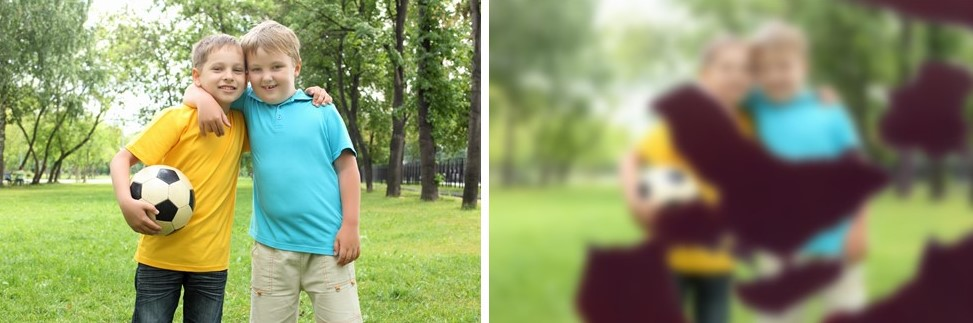
\includegraphics[width=1\linewidth]{drSymptoms.jpg} \caption{(α')Οπτική ενός υγιούς ατόμου (β')Οπτική ενός ατόμου με Διαβητική Αμφιβληστροειδοπάθεια}
\label{figure:drSymptoms}  
\end{figure}

Όσον αφορά τη διάγνωση, σημαντικότερα σημάδια της ασθένειας αποτελούν τα μικροανευρίσματα, τα νεοαγγεία, οι αιμορραγίες, τα σκληρά  εξιδρώματα και οι βαμβακόμορφες κηλίδες \cite{Nayak}\cite{Acharya}. Στην εικόνα \ref{figure:signs} επισημαίνονται τα συμπτώματα της ασθένειας.


\begin{figure}[!h]
    \centering
      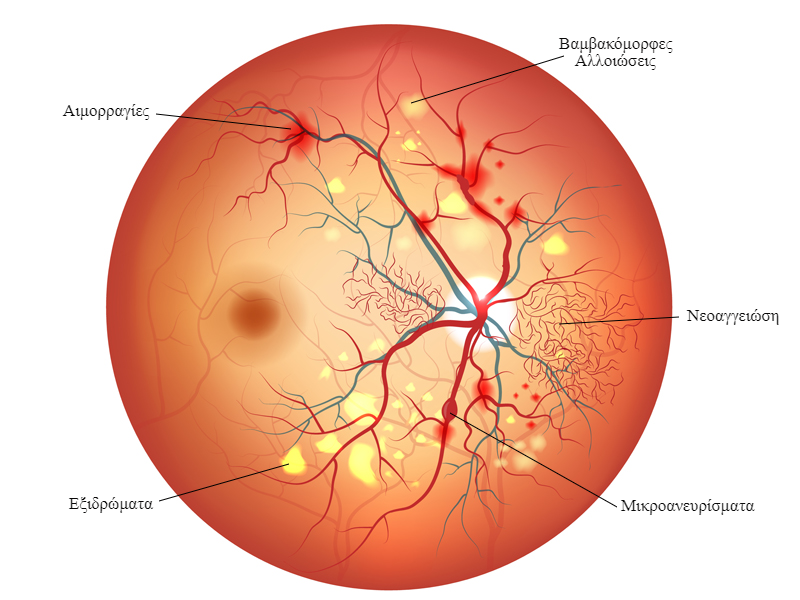
\includegraphics[width=0.7\linewidth]{signs.png} \caption{Συμπτώματα της Διαβητικής Αμφιβληστροειδοπάθειας}
       \label{figure:signs}    
  \end{figure}



\section{Διάρθρωση της Εργασίας}
Tο \textbf{Κεφάλαιο 1} αποτελεί την εισαγωγή στη διπλωματική εργασία. Δίνεται ενδεικτικά μία περιγραφή του προβλήματος. Στη συνέχεια, αναλύεται ο στόχος της διπλωματικής και περιγράφεται η ασθένεια της Διαβητικής Αμφιβληστροειδοπάθειας. 

Στο \textbf{Κεφάλαιο 2} δίνονται συνοπτικά οι δύο  σημαντικότερες  προσεγγίσεις που απαντώνται στη βιβλιογραφία για την αυτόματη ανίχνευση της rDR ή της DR και παρουσιάζονται κάποιες σχετικές εργασίες.

Στο \textbf{Κεφάλαιο 3} εξηγούνται σημαντικές έννοιες και δίνονται πληροφορίες για τα τεχνητά νευρωνικά δίκτυα, τα συνελικτικά νευρωνικά δίκτυα και τις Μηχανές Διανυσμάτων Υποστήριξης. Επιπλέον, γίνεται αναφορά στο νευρωνικό Inception V3 και περιγράφονται μερικές από τις τεχνικές σχεδίασης του. Τέλος, παρουσιάζονται τα εργαλεία που χρησιμοποιήθηκαν.

Στο \textbf{Κεφάλαιο 4} παρουσιάζονται συνοπτικά τα σύνολα δεδομένων Kaggle και Messidor 2. Επίσης, παρουσιάζεται ο αλγόριθμος που χρησιμοποιήθηκε για τη μείωση των διαστάσεων των εικόνων.

Στο \textbf{Κεφάλαιο 5} παρουσιάζονται οι μέθοδοι
που απέδωσαν τα καλύτερα αποτελέσματα για την  ανίχνευση της rDR ενώ παράλληλα γίνεται μία  αναφορά σε προσπάθειες που επέφεραν ισάξια ή κατώτερα αποτελέσματα.

Στο \textbf{Κεφάλαιο 6} γίνεται αναφορά στις μετρικές που επιλέχθηκαν για την αξιολόγηση της παρούσας διπλωματικής και περιγράφεται ο τρόπος υπολογισμού τους.

Στο \textbf{Κεφάλαιο 7} παρουσιάζονται και σχολιάζονται τα αποτελέσματα των καλύτερων μεθόδων. Επίσης, εξηγείται η μέθοδος που ακολουθήθηκε για την οπτικοποίηση των περιοχών, που σύμφωνα με το νευρωνικό, εντοπίζεται η ασθένεια και δίνονται κάποια παραδείγματα οπτικοποίησης. Τέλος, γίνεται αναφορά σε μελλοντικές επεκτάσεις.



\chapter{Βιβλιογραφική Επισκόπηση }
\label{chap:2}
\thispagestyle{plain}


\section{Υπάρχουσες Προσεγγίσεις}
\label{sec:2.1}
Στη βιβλιογραφία απαντώνται δύο προσεγγίσεις για την αυτόματα ανίχνευση της Διαβητικής Αμφιβληστροειδοπάθειας. Στην πρώτη προσέγγιση, γίνεται εξαγωγή συγκεκριμένων χαρακτηριστικών της ασθένειας(χωρίς τη χρήση νευρωνικών δικτύων). Τα χαρακτηριστικά που εξάγονται συνήθως είναι: σκληρά εξιδρώματα, μικροανευρίσματα, νεοαγγεία και βαμβακόμορφες κηλίδες. Επιπλέον εξάγονται κάποια χαρακτηριστικά της εικόνας πχ αντίθεση και διακύμανση και κάποια στοιχεία της δομής του αμφιβληστροειδούς πχ αγγεία, οπτικός δίσκος κα. Συνήθως σε αυτή τη προσέγγιση αρχικά γίνεται επεξεργασία των εικόνων ώστε να επιτευχθεί ενίσχυση των χαρακτηριστικών τους και στη συνέχεια εφαρμόζονται διάφορες τεχνικές για την εξαγωγή των εν λόγω χαρακτηριστικών\cite{Nayak}. Για την τελική πρόβλεψη εφαρμόζονται πληθώρα αλγορίθμων όπως μηχανές διανυσμάτων υποστήριξης(SVM), κ - κοντινότεροι γείτονες, τεχνητά νευρωνικά δίκτυα, δέντρα απόφασης κα. Επιπλέον, η τελική πρόβλεψη μπορεί να δοθεί βάση κάποιων κριτηρίων μεγέθους και αριθμού των χαρακτηριστικών της ασθένειας που ανιχνεύθηκαν. Οι κλάσεις ταξινόμησης μπορεί να είναι: έχει/δεν έχει rDr, έχει/δεν έχει DR ή ποιο βαθμό DR έχει(multi-class classification). Σε κάποιες εργασίες εξάγονται μόνο τα χαρακτηριστικά της ασθένειας, παραλείποντας τη διαδικασία ανίχνευσης της. Ωστόσο και αυτές οι προσεγγίσεις παίζουν σημαντικό ρόλο στη λύση του προβλήματος καθώς η κύρια δυσκολία της πρώτης προσέγγισης είναι η εξαγωγή των χαρακτηριστικών και όχι τόσο η επιλογή του τελικού ταξινομητή.

 
 Στη δεύτερη προσέγγιση γίνεται χρήση βαθιών συνελικτικών νευρωνικών δικτύων τα οποία δέχονται ως είσοδο ένα μεγάλο σύνολο εικόνων και την αντίστοιχη κλάση στην οποία ανήκουν. Το δίκτυο μαθαίνει τα χαρακτηριστικά της ασθένειας από το συνδυασμό εικόνας και της αντίστοιχης κλάσης. Το νευρωνικό δίκτυο θα μπορούσε να περιγραφεί ως μία συνάρτηση με πολλές παραμέτρους, οι οποίες προσαρμόζονται έτσι ώστε να προβλέπουν την κλάση που ανήκει κάθε εικόνα.  Επιπλέον, απαντώνται μετασχηματισμοί της εικόνας για την ενίσχυση των χαρακτηριστικών της, ενώ συνήθως γίνεται χρήση της τεχνικής αύξησης δεδομένων για την αποφυγή της υπερεκπαίδευσης και την αύξηση της επίδοσης του μοντέλου. Και σε αυτή την προσέγγιση οι κλάσεις ταξινόμησης μπορεί να είναι: έχει/δεν έχει rDr, έχει/δεν έχει DR ή ποιο βαθμό DR έχει(multi-class classification).

Οι διαφορές των δύο προσεγγίσεων δεν περιορίζονται μόνο στον τρόπο εξαγωγής των χαρακτηριστικών. Μία αρκετά σημαντική διαφορά είναι ο αριθμός των εικόνων που απαιτείται στην κάθε προσέγγιση, με την πρώτη να απαιτεί μερικές εκατοντάδες εικόνες ενώ η δεύτερη μερικές δεκάδες χιλιάδες εικόνες. Όπως είναι γνωστό τα συνελικτικά νευρωνικά δίκτυα απαιτούν αρκετές εικόνες ώστε να εκπαιδευτούν και να παρουσιάσουν καλά αποτελέσματα ενώ ο μεγάλος αριθμός εικόνων μειώνει την πιθανότητα για υπερεκπαίδευση. Έτσι, η δεύτερη προσέγγιση με συνελικτικα νευρωνικά δίκτυα απαιτεί την εύρεση ενός μεγάλου συνόλου δεδομένων ενώ συγχρόνως πολύ σημαντική είναι και η σωστή ανάθεση των εικόνων στις κλάσεις. 
Επιπλέον, ανάλογα με την κάμερα λήψης, τις συνθήκες φωτισμού και τη φυλή των εξεταζόμενων παρουσιάζονται μεγάλες διαφορές στις εικόνες του αμφιβληστροειδούς. Συνήθως στη πρώτη προσέγγιση παρατηρούνται πολύ καλά αποτελέσματα στο σύνολο δεδομένων που βασίστηκε ο αλγόριθμος ωστόσο δεν συμβαίνει το ίδιο για άλλα σύνολα δεδομένων. Αντίθετα,  τα  συνελικτικά νευρωνικά δίκτυα μπορούν να εκπαιδευτούν κατά τέτοιο τρόπο ώστε να γενικεύονται σε διάφορα σύνολα δεδομένων. Παρακάτω, παρουσιάζονται κάποιες σχετικές εργασίες με την ανίχνευση της ασθένειας.

\section{Παραδείγματα Βιβλιογραφίας}
\label{sec:2.2}

Στο Nayak et al\cite{Nayak} γίνεται χρήση τεχνικών επεξεργασίας εικόνας όπως προσαρμοσμένη εξισορρόπηση ιστογράμματος(adaptive histogram equalization), μορφολογικές τεχνικές για την ανίχνευση αιμοφόρων αγγείων και σκληρών εξιδρωμάτων και μέθοδοι ανάλυσης υφής για την μέτρηση της διακύμανσης της έντασης της εικόνας(αντίθεση). Αφού υπολογιστούν τα παραπάνω, δίνονται ως είσοδο σε ένα τεχνητό νευρωνικό δίκτυο. Συγκεκριμένα το νευρωνικό δέχεται ως είσοδο  το εμβαδόν και τη περίμετρο των αιμοφόρων αγγείων, το εμβαδόν των εξιδρωμάτων και το μέτρο της αντίθεσης ενώ η έξοδος  προβλέπει τρεις κλάσεις: norm, non proliferative DR, proliferative DR. Η μέθοδος πετυχαίνει ακρίβεια 93\%, ευαισθησία 90\% και εξειδίκευση 100\%. Για τη μέθοδο αυτή χρησιμοποιήθηκαν 140 δείγματα.



Στο Acharya et al\cite{Acharya2} χρησιμοποιούνται μη γραμμικά χαρακτηριστικά Higher-order spectra(HOS) ως είσοδο σε ταξινομητή SVM που πραγματοποιεί ταξινόμηση πέντε κλάσεων normal, mild, moderate, severe και proliferative DR. Συγκεκριμένα, στις εικόνες εφαρμόζεται η τεχνική εξισορρόπησης ιστογράμματος(Histogram equalization) για ενίσχυση της αντίθεσης, έπειτα οι εικόνες μετατρέπονται σε κλίμακα του γκρι και μετασχηματίζονται σε 1D δεδομένα με το μετασχηματισμό Radon. Τέλος, υπολογίζονται τα HOS χαρακτηριστικά και δίνονται ως είσοδο στον ταξινομητή. Για τη μέθοδο αυτή χρησιμοποιήθηκαν 300 δείγματα. Η μέθοδος πετυχαίνει ευαισθησία 82\% και εξειδίκευση 88\%.


Στο Priya et al \cite{Priya} συγκρίνεται η χρήση Πιθανοτικών νευρωνικών δικτύων(Probabilistic Neural network - PNN) και η χρήση Μηχανών διανυσμάτων υποστήριξης (SVM) για την τελική ταξινόμηση της ασθένειας. Όπως διαπιστώθηκε η χρήση SVM ως ταξινομητή υπερέχει έναντι του μοντέλου PNN, με το πρώτο να πετυχαίνει 97\% ακρίβεια ενώ το δεύτερο 89\%. 


Στο Gulshan et al \cite{Gulshan} στο οποίο βασίστηκε και η παρούσα διπλωματική χρησιμοποιήθηκε το νευρωνικό Inception V3. Έγινε χρήση ενός ιδιωτικού συνόλου δεδομένων με 128175 εικόνες, κάθε εικόνα  αξιολογήθηκε 3 με 7 φορές από ειδικούς οφθαλμίατρους για την αντιστοίχιση τους στις κλάσεις no, mild, moderate, severe, και proliferative DR και την ύπαρξη ή όχι οιδήματος της ωχράς κηλίδας. Επιπλέον, έγινε αύξηση των δεδομένων κατά την εκπαίδευση με αλλαγή της αντίθεσης, της φωτεινότητας, της απόχρωσης και του κορεσμού. Τέλος, υλοποιήθηκε ensemble 10 μοντέλων, με την τελική απόφαση να λαμβάνεται ως  ένας γραμμικός μέσος όρος των προβλέψεων. Επιπροσθέτως, έγιναν πειράματα με διαφορετικό αριθμό δειγμάτων εκπαίδευσης και αποδείχθηκε ότι μετά τα 55000 περίπου δείγματα εκπαίδευσης, με σταθερό σύνολο επικύρωσης 24360 εικόνες, δεν παρατηρείται βελτίωση της απόδοσης του μοντέλου. Η υλοποίηση πετυχαίνει άκρως εντυπωσιακά αποτελέσματα με AUC 0.991 για το ιδιωτικό σύνολο δεδομένων και 0.99 για το σύνολο δεδομένων Messidor 2.

Στο  Gargeya et al \cite{Gargeya} γίνεται χρήση ενός νευρωνικού με Residual αρχιτεκτονική. Η συγκεκριμένη αρχιτεκτονική περιγράφεται από την εξίσωση \ref{eq:resi}

\begin{equation} \label{eq:resi}
x_{l} = conv_{l}(x_{l-1}) + x_{l-1}
\end{equation}

όπου το $conv_{l}$ αναπαριστά το συνελικτικό επίπεδο $l$ και η έξοδος $x_{l}$ δίνεται ως ένα άθροισμα της εξόδου του συνελικτικού επιπέδου $l$ δηλαδή $conv_{l}(x_{l-1})$ και της εξόδου του προηγούμενου συνελικτικού επιπέδου δηλαδή $x_{l-1}$
Για την εκπαίδευση χρησιμοποιήθηκε ένα σύνολο δεδομένων με 75137, το οποίο χωρίστηκε στα σύνολα εκπαίδευσης, επικύρωσης και ελέγχου και οι εικόνες αξιολογήθηκαν από ειδικούς ώστε να αποδοθεί σε κάθε εικόνα η αντίστοιχη κλάση στην οποία ανήκει. Επίσης, χρησιμοποιήθηκε το Messidor 2 ως ένα επιπλέον σύνολο ελέγχου. Επιπροσθέτως, έγινε αύξηση δεδομένων με χρήση περιστροφής και προσαρμογής φωτεινότητας και αντίθεσης. Το μοντέλο πετυχαίνει 0.97 AUC στο σύνολο ελέγχου του βασικού συνόλου δεδομένων  και 0.94 στο Messidor 2. Στη συγκεκριμένη προσέγγιση ανιχνεύεται η DR, όχι η referable DR.


Στο Lin et al\cite{Lin} προτείνεται η χρήση εικόνων εντροπίας ως είσοδο στο νευρωνικό αφού πρώτα μετατραπούν σε εικόνες κλίμακας του γκρι ενώ στο Seth et al \cite{Seth} προτείνεται η χρήση συλλεκτικών νευρωνικών δικτύων με ταξινομητή SVM με γραμμικό πυρήνα. Ως είσοδος στο μοντέλο SVM δίνεται η έξοδος του προτελευταίου πλήρες συνδεδεμένου επιπέδου του νευρωνικού με 1024 νευρώνες.


\thispagestyle{plain}
\chapter{Θεωρητικό Υπόβαθρο και Εργαλεία}
\label{chap:3}

\section{Θεωρητικό Υπόβαθρο}
\label{sec:3.1}

\subsection{Βασικοί ορισμοί}
\label{subsec:3.1.1}

Με τον όρο \textit{Τεχνητή Νοημοσύνη - Artificial Intelligence} περιγράφεται η ικανότητα των μηχανών να μιμούνται ορισμένες λειτουργίες του ανθρώπινου εγκεφάλου όπως  μάθηση, προσαρμοστικότητα, εξαγωγή συμπερασμάτων, κατανόηση από συμφραζόμενα, επίλυση προβλημάτων κα.

 Η \textit{Μηχανική Μάθηση - Machine Learning} είναι υποσύνολο της Τεχνητής Νοημοσύνης και αποτελεί πεδίο μελέτης στο οποίο δίνεται η ικανότητα στους υπολογιστές να μαθαίνουν, χωρίς να έχουν προγραμματιστεί ρητά για την εκάστοτε λειτουργία. 
 
Μία από τις ευρέως γνωστές εργασίες Μηχανικής Μάθησης αποτελεί η \textit{Επιβλεπόμενη Μάθηση - Supervised Learning}. Στους αλγόριθμους Επιβλεπόμενης Μάθησης δίνεται ένα σύνολο δεδομένων και η επιθυμητή έξοδος. Ο αλγόριθμος προσπαθεί να εντοπίσει τις συσχετίσεις μεταξύ εισόδου και εξόδου. Μετά την εκπαίδευση, δηλαδή την προσπάθεια εύρεσης των συσχετίσεων εισόδου-εξόδου, δημιουργείται ένα μοντέλο το οποίο αναμένεται να μπορεί να προβλέπει την έξοδο για νέα δεδομένα στην είσοδο. Το μοντέλο πρέπει να γενικεύει αρκετά και όχι να ‘αποστηθίζει’ τα δεδομένα στα οποία εκπαιδεύτηκε, διαφορετικά δεν θα μπορεί να προβλέψει σωστά την έξοδο για νέες εισόδους. 


Επιγραμματικά, οι σημαντικότεροι αλγόριθμοι Επιβλεπόμενης Μάθησης είναι οι εξής: Τεχνητά Νευρωνικά Δίκτυα(Artificial Neural Networks), Μηχανές Διανυσμάτων Υποστήριξης(Support Vector Machines), Γραμμική Παλινδρόμηση(Linear Regression), Λογιστική Παλινδρόμηση(Logistic Regression), Δίκτυα Bayes(Naive Bayes), Γραμμική Διακριτική Ανάλυση(Linear Discriminant Analysis), Δέντρα Απόφασης(Decision Trees), Κ - κοντινότεροι Γείτονες(K-nearest Neighbor) και Εκμάθηση με μέτρο ομοιότητας(Similarity learning). 


\subsection{Τεχνητά Νευρωνικά Δίκτυα(Artificial Neural Network)}
\label{subsec:3.1.2}


Τα Τεχνητά Νευρωνικά Δίκτυα είναι υπολογιστικά συστήματα εμπνευσμένα  από βιολογικά νευρικά δίκτυα τα οποία συνιστούν τον εγκέφαλο των ζώων.  Αποτελούνται από επίπεδα
με συνδεδεμένους κόμβους που ονομάζονται νευρώνες ενώ οι συνδέσεις ανάμεσα στους νευρώνες ονομάζονται ακμές. Οι νευρώνες ενός επιπέδου είναι συνδεδεμένοι με όλους ή κάποιους από τους νευρώνες του προηγούμενου και του επόμενου επιπέδου.


Κάθε νευρώνας δέχεται ένα σύνολο αριθμητικών εισόδων είτε από άλλους νευρώνες, είτε από το περιβάλλον, με βάση αυτές τις εισόδους εκτελεί έναν υπολογισμό και παράγει μία έξοδο. Στην εικόνα \ref{figure:basicann} παρουσιάζεται μία απλή δομή ANN με τρία επίπεδα: το επίπεδο εισόδου(Input Layer), το κρυμμένο επίπεδο(Hidden Layer) και το επίπεδο εξόδου(Output Layer). Ωστόσο, σε μία πιο σύνθετη μορφή συναντάμε περισσότερα από ένα κρυφά επίπεδα. Επίσης, δεν υπάρχει περιορισμός στον αριθμό των νευρώνων σε κάθε επίπεδο.



\begin{figure}[!h]
    \centering
      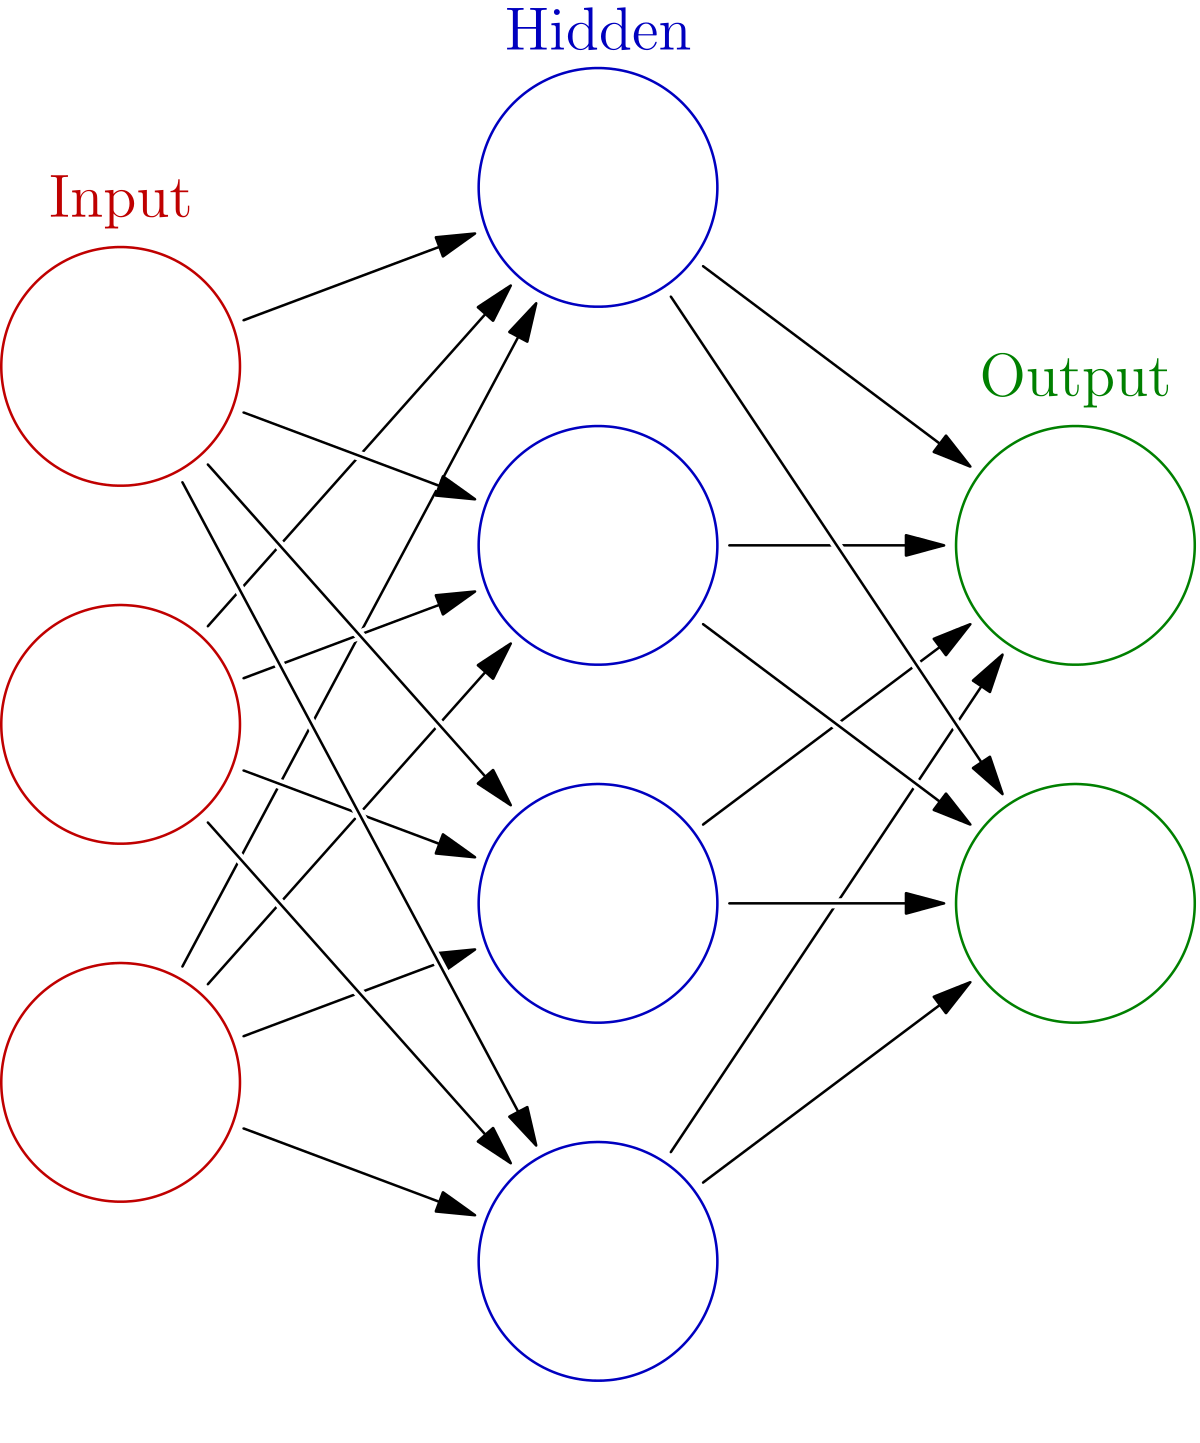
\includegraphics[width=0.3\linewidth]{basic_ann.png} \caption{Βασική δομή ANN}
          \label{figure:basicann}  

  \end{figure}



Ένα ANN μπορεί να περιγραφεί ως ένας κατευθυνόμενος γράφος που κάθε κόμβος $i$ εκτελεί μία συνάρτηση μεταφοράς $f_{i}$ της μορφής: \cite{Yao}




\begin{equation} \label{eq:1}
y_{i} = f_{i}(\sum_{j=1}^{n}w_{ij}x_{j}+\theta_{i})
\end{equation}


όπου $y_{i}$ είναι η έξοδος του κόμβου $i$, $x_{j}$ είναι η $j^{th}$ είσοδος στο $i$ κόμβο, $w_{ij}$ είναι το βάρος που συνδέει τους κόμβους $i$ και $j$ και $θ_{i}$(ή bias) είναι το κατώφλι του κόμβου μέσω του οποίου μπορεί να ρυθμιστεί περαιτέρω η ενεργοποίηση του νευρώνα. Η συνάρτηση $f_{i}$ είναι συνήθως μη γραμμική και ονομάζεται συνάρτηση ενεργοποίησης. Κάποιες συνηθισμένες μορφές της είναι οι \ref{eq:Rectifier}, \ref{eq:Sigmoid}, \ref{eq:tanh}.

Ανόρθωσης(Rectifier): 
\begin{equation} \label{eq:Rectifier}
φ(x) = max(0, x)
\end{equation}
\\


Λογιστική σιγμοειδής(Logistic Sigmoid): 
\begin{equation} \label{eq:Sigmoid}
φ(x) = \frac{1}{1+ e^{-x}}
\end{equation}
\\


Υπερβολική εφαπτομένη(Hyperbolic tangent): 
\begin{equation} \label{eq:tanh}
φ(x) = tanh(x)
\end{equation}

Ξεχωριστό ρόλο επιτελούν οι νευρώνες εισόδου, οι οποίοι δεν επιτελούν κάποιο υπολογισμό αλλά αναλαμβάνουν να τροφοδοτήσουν το δίκτυο με την είσοδο και οι νευρώνες εξόδου που διοχετεύουν στο περιβάλλον τις τελικές αριθμητικές εξόδους του δικτύου.

 
Το ANN μετά από μία διαδικασία που ονομάζεται εκπαίδευση θα πρέπει να μπορεί να προβλέπει την έξοδο, για νέες εισόδους. Η εκπαίδευση περιλαμβάνει τη σωστή ρύθμιση των βαρών και του κατωφλίου που αναφέρθηκαν στην \ref{eq:1}, σε τιμές κατάλληλες ώστε να επιλύεται με επαρκή επιτυχία το προς εξέταση πρόβλημα. Αυτό γίνεται με μία διαδικασία ανάδρασης που ονομάζεται backpropagation.


Αρχικά, τα δεδομένα περνάνε από όλα τα επίπεδα και υπολογίζεται η πρόβλεψη του δικτύου. Στη συνέχεια, συγκρίνεται η πραγματική κλάση στην οποία ανήκουν τα δεδομένα με την πρόβλεψη του δικτύου και υπολογίζεται το διάνυσμα σφάλματος. Τέλος, το διάνυσμα σφάλματος ανατροφοδοτείται διαδοχικά στα προηγούμενα επίπεδα, από το επίπεδο εξόδου στο επίπεδο εισόδου, και οι νευρώνες κάθε επιπέδου αναπροσαρμόζουν τις παραμέτρους προς την κατεύθυνση μείωσης του σφάλματος. Αφού το δίκτυο εκπαιδευτεί, τα βάρη και η παράμετρος κατωφλίου παγώνουν και πια το μοντέλο είναι έτοιμο να κάνει προβλέψεις για νέες εισόδους διαφορετικές από αυτές στις οποίες εκπαιδεύτηκε.
    




\subsection{Συνελικτικά Νευρωνικά Δίκτυα(Convolutional Neural Network)}
\label{subsec:3.1.3}



Προηγουμένως, έγινε μια συνοπτική ανάλυση των ANN ώστε να τεθούν οι βάσεις για την περιγραφή των \textit{Συνελικτικών Νευρωνικών Δικτύων} τα οποία χρησιμοποιούνται στην παρούσα διπλωματική. Τα \textit{Συνελικτικά Νευρωνικά Δίκτυα} είναι μία ευρέως χρησιμοποιούμενη αρχιτεκτονική της Μηχανικής Μάθησης και αποτελεί κατηγορία των Τεχνητών Νευρωνικών Δικτύων.
Αποτελούνται από ένα ή περισσότερα επίπεδα συνέλιξης, ακολουθούμενα συνήθως από επίπεδα υποδειγματοληψίας. Τα τελευταία επίπεδα του δικτύου συνήθως περιέχουν πλήρη συνδεδεμένα επίπεδα για την ταξινόμηση των εισόδων στις κλάσεις.
Η περιγραφή των παραπάνω επιπέδων θα δοθεί σε επόμενες παραγράφους.


Συνοπτικά, η λειτουργιά των CNN μπορεί να περιγραφεί ως εξής: Αρχικά, οι εικόνες εισόδου διέρχονται από τα διάφορα επίπεδα και το νευρωνικό  εξάγει σταδιακά όλο και πιο σύνθετα τοπικά χαρακτηριστικά μέσω της προσαρμογής των διαφόρων φίλτρων των συνελικτικών επιπέδων. Στα πρώτα συνελικτικά επίπεδα το δίκτυο μαθαίνει κάποιες απλές δομές ενώ σε μεγαλύτερο βάθος εξάγονται πιο σύνθετα χαρακτηριστικά. Για παράδειγμα, αν η είσοδος  είναι μία εικόνα, στα πρώτα επίπεδα εξάγονται ακμές και βασικά σχήματα ενώ σε υψηλότερα επίπεδα μπορεί να εξαχθούν σύνθετες δομές, για παράδειγμα ψηφία, γράμματα και πρόσωπα. Έπειτα, τα χαρακτηριστικά που εξήχθησαν αντιστοιχίζονται στους χάρτες χαρακτηριστικών(feature maps) που αποτελούν μια βιβλιοθήκη των χαρακτηριστικών  που εμφανίζονται στις εικόνες μιας κλάσης. Μέσω της παραπάνω αντιστοίχισης είναι δυνατή η πρόβλεψη της εξόδου για νέες εικόνες στην είσοδο. Στην εικόνα \ref{figure:convNet} παρουσιάζεται μία τυπική δομή ενός συνελικτικού δικτύου.




\begin{figure}[!h]
    \centering
      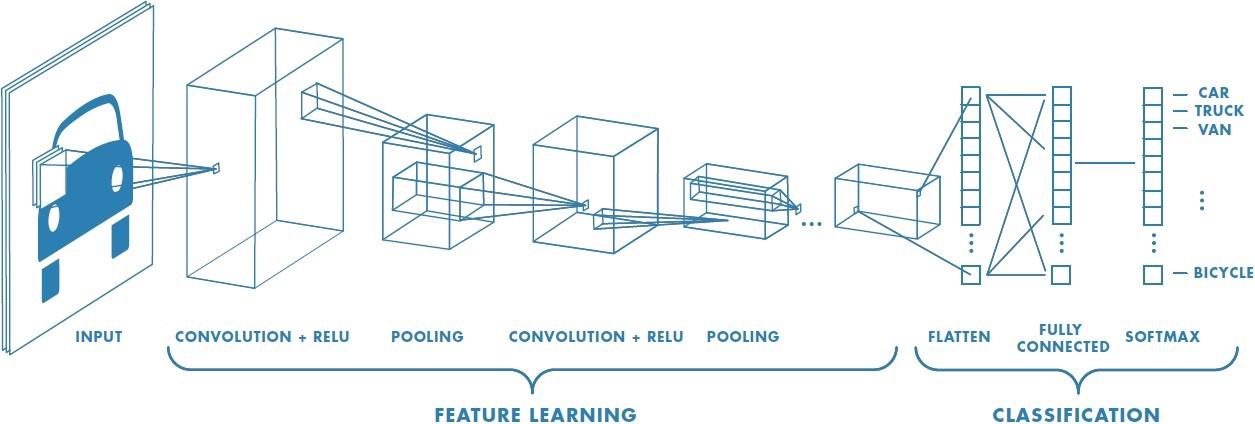
\includegraphics[width=0.95\linewidth]{convNet.jpeg} \caption{Τυπική δομή ενός Συνελικτικού Δικτύου}
      \label{figure:convNet}    
  \end{figure}


Τα Συνελικτικα Νευρωνικα Δικτυα προτιμουνται έναντι των Πλήρως Συνδεδεμένων Δικτύων, δηλαδή των δικτύων στα οποία οι νευρώνες ενός επιπέδου είναι συνδεδεμένοι με όλους τους νευρώνες του προηγούμενου και του επόμενου επιπέδου, λόγω του μικρότερου αριθμού παραμέτρων που απαιτούν. Για παράδειγμα, ένα πλήρως συνδεδεμένο δίκτυο για μία μικρή εικόνα 200x200 απαιτεί 40000 παραμέτρους για κάθε νευρώνα στο επόμενο επίπεδο. Εν αντιθέσει, ένα συνελικτικό επίπεδο περιέχει σταθερά φίλτρα διαφόρων διαστάσεων ανεξάρτητα από την είσοδο. Το Νευρωνικά Συνελικτικά Δίκτυα αποτελούνται από διάφορα δομικά στοιχεία τα οποία τελούν διαφορές λειτουργιές. Παρακάτω γίνεται μια συνοπτική παρουσίαση μερικών σημαντικών δομικών στοιχείων που εμφανίζονται στα Συνελεκτικό Δίκτυα και συγκεκριμένα στο Inception V3, το οποίο χρησιμοποιήθηκε στην παρούσα διπλωματική.


\subsubsection{Συνελικτικο Επίπεδο(Convolutional Layer)}
\label{subsubsec:3.1.3.1}


Ένα συνελικτικό επίπεδο περιέχει φίλτρα των οποίων οι τιμές καθορίζονται κατά την εκπαίδευση. Τα φίλτρα συνεχίζονται με την είσοδο και παράγονται οι χάρτες χαρακτηριστικών, οι οποίοι περιέχουν τις θέσεις ενεργοποίησης των φίλτρων. Ουσιαστικά το φίλτρο ολισθαίνει πάνω στην είσοδο και το αποτέλεσμα της συνέλιξης σε μία συγκεκριμένη χωρική θέση της εισόδου υπολογίζεται ως το γινόμενο(στοιχείο προς στοιχείο) του φίλτρου και ενός παραθύρου της εικόνας ίδιων διαστάσεων με το φίλτρο και με κεντρικό εικονοστοιχείο το σημείο στη συγκεκριμένη χωρική θέση. Οι διαστάσεις των φίλτρων(ύψος και πλάτος), πρέπει να είναι μικρότερες από αυτές της εικόνας.
 
 
Έτσι, για μία εικόνα MxNxC όπου MxN το ύψος και πλάτος της εικόνας αντίστοιχα και C ο αριθμός των καναλιών της, η συνέλιξη με C1 φίλτρα M1xN1 θα δώσει ως αποτέλεσμα χάρτες χαρακτηριστικών με διαστάσεις (Μ-Μ1+1)x(N-N1+1)xC1. Όπως είναι φανερό το ύψος και το πλάτος της εικόνας θα μειωθούν ανάλογα με το ύψος και το πλάτος του φίλτρου συνέλιξης. Η μείωση αυτή οφείλεται στα άκρα της εικόνες καθώς για να είναι δυνατή η συνέλιξη σε μία θέση της εικόνας θα πρέπει να υπάρχουν οι αντίστοιχοι γείτονες για να πολλαπλασιαστεί το φίλτρο. Επίσης, ο αριθμός των καναλιών αλλάζει από C σε C1. Η αλλαγή αυτή προκύπτει καθώς τα C1 φίλτρα διάστασης M1xN1 στην πραγματικότητα είναι C1 φίλτρα διάστασης M1xN1xC.




Στην \ref{figure:conv} απεικονίζεται η συνέλιξη του φίλτρου Κ με την εικόνα εισόδου I.


\begin{figure}[!h]
    \centering
      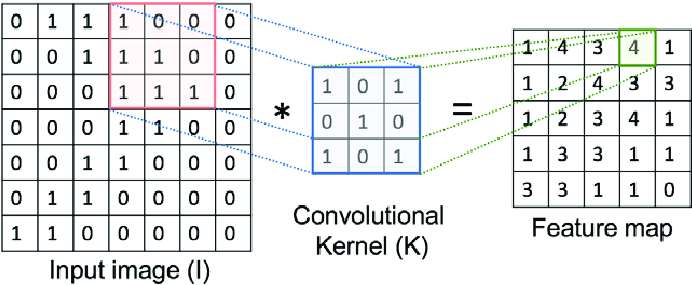
\includegraphics[width=0.6\linewidth]{conv.png} \caption{Συνέλιξη της εικόνας I με το φίλτρο K}
\label{figure:conv}  
\end{figure}


\subsubsection{Επίπεδο Υποδειγματοληψίας(Pooling layer)}
\label{subsubsec:3.1.3.2}


Το επίπεδο Υποδειγματοληψίας χρησιμοποιείται για τη μείωση της χωρικών διαστάσεων στους χάρτες χαρακτηριστικών και απαντάται κυρίως μετά από συνελεκτικά επίπεδα. Η μείωση των χωρικών διαστάσεων έχει σκοπό τη μείωση του αριθμού των παραμέτρων και των υπολογισμών. Επιπλέον, μειώνεται η πιθανότητα για  υπερεκπαίδευση. Οι δυο κύριες μέθοδοι υποδειγματοληψίας είναι η υποδειγματοληψία μεγίστου και η υποδειγματοληψία μέσου όρου. Στην πρώτη επιλέγεται η μέγιστη τιμή για ένα παράθυρο της εικόνας, ενώ στη δεύτερη υπολογίζεται ο μέσος όρος των τιμών του κάθε παραθύρου. Στην εικόνα \ref{figure:maxAvgPool} παρουσιάζονται οι  συνηθέστεροι μέθοδοι χωρικής υποδειγματοληψίας. Να σημειωθεί ότι το επίπεδο υποδειγματοληψίας εφαρμόζεται συνήθως στις διαστάσεις [ύψος x πλάτος] της εικόνας και όχι στη τρίτη διάσταση.



\begin{figure}[!h]
    \centering
      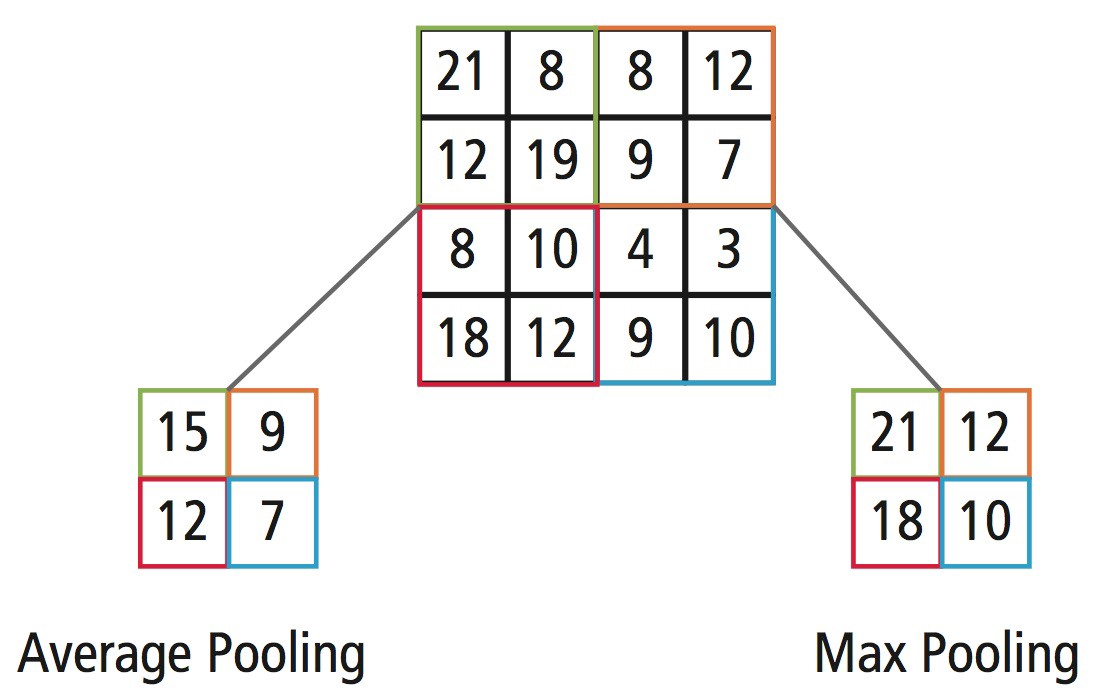
\includegraphics[width=0.6\linewidth]{maxAvgPool.jpeg} \caption{Υποδειγματοληψία μέσης (αριστερά) και μέγιστης (δεξιά) τιμής}
      \label{figure:maxAvgPool}    
  \end{figure}


\subsubsection{Καθολικό Επίπεδο Υποδειγματοληψίας(Global Pooling layer)}
\label{subsubsec:3.1.3.3}
Αποτελεί μία ειδική περίπτωση υποδειγματοληψίας καθώς ως παράθυρο υποδειγματοληψίας λαμβάνεται όλη η εικόνα. Όποτε, μία εικόνα με διαστάσεις (ύψος)x(πλάτος)x(κανάλια) μετατρέπεται σε (1)x(1)x(κανάλια). Συνήθως, χρησιμοποιείται μετά το τελευταίο συνελικτικό επίπεδο αντί της χρήσης ενός πλήρες συνδεδεμένου επιπέδου. Η πιο συνηθισμένη καθολική υποδειγματοληψία είναι η καθολική υποδειγματοληψία μέσου όρου που παρουσιάζεται στην εικόνα \ref{figure:gap2}



\begin{figure}[!h]
    \centering
      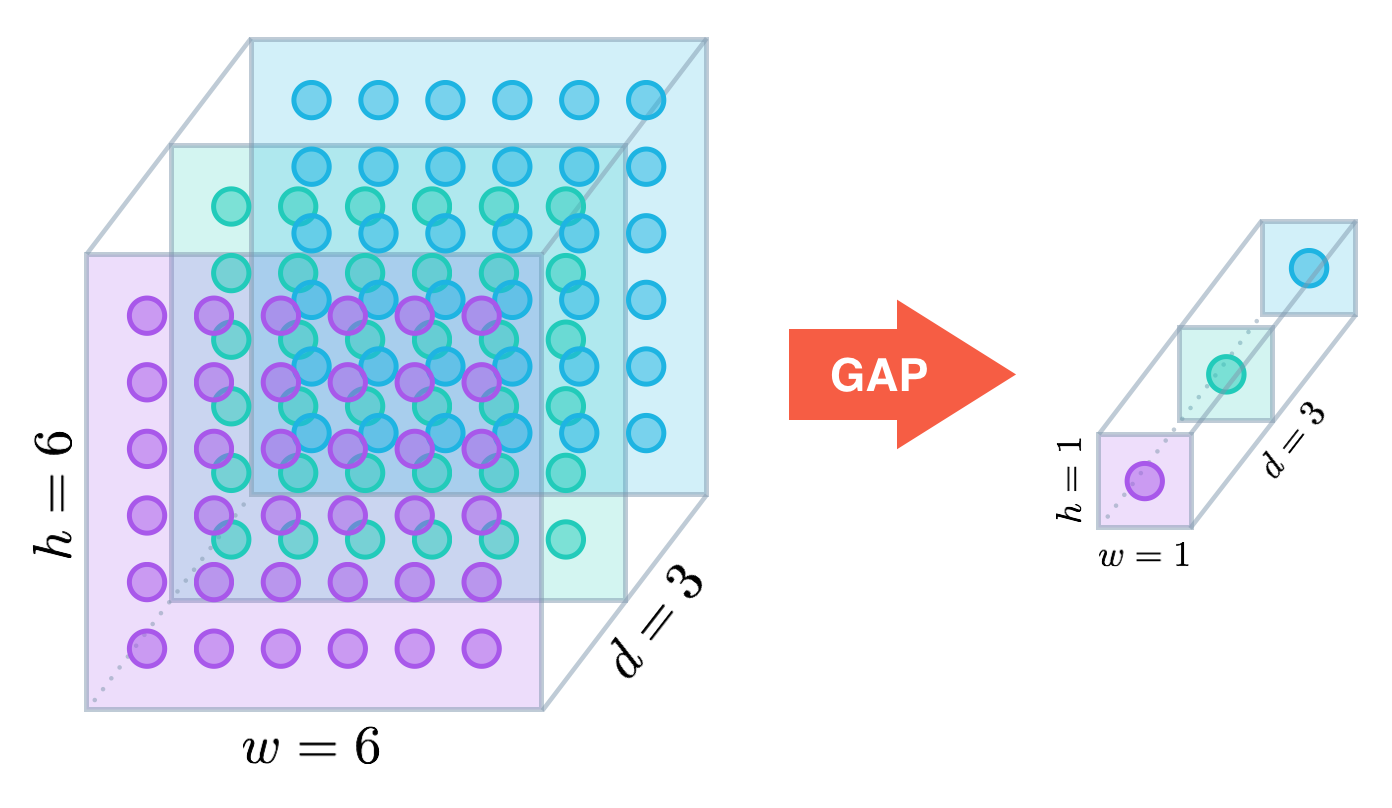
\includegraphics[width=0.6\linewidth]{gap2.png} \caption{Καθολική Υποδειγματοληψεία μέσου όρου}
      \label{figure:gap2}    
  \end{figure}


\subsubsection{Πλήρες Συνδεδομένο επίπεδο(Fully Connected Layer)}
\label{subsubsec:3.1.3.4}


Αποτελείται από  νευρώνες κάθε ένας εκ των οποίων συνδέεται με τους νευρώνες του προηγούμενου αλλά και του επόμενου πλήρους συνδεδεμένου επιπέδου(αν υπάρχουν). Συνήθως παρατηρείται μια ακολουθία από πλήρως συνδεδεμένα επίπεδα τα όποια τοποθετούνται πάντα μετά το τελευταίο συνελικτικό επίπεδο και αποτελούν το τελικό στάδιο για την ταξινόμηση των εικόνων. Το τελευταίο πλήρες συνδεδεμένο επίπεδο περιέχει τόσους νευρώνες όσες και οι κλάσεις του προβλήματος ταξινόμησης. Στην εικόνα \ref{figure:fullyconncted} παρουσιάζεται ένα πλήρες συνδεμένο επίπεδο.


\begin{figure}[!h]
    \centering
      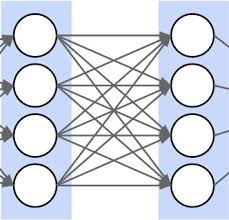
\includegraphics[width=0.2\linewidth]{fullyconncted.jpg} \caption{Πλήρες Συνδεδεμένο Επίπεδο}
\label{figure:fullyconncted}  
\end{figure}



\subsubsection{Επίπεδο Συνένωσης(Concatenate)}
\label{subsubsec:3.1.3.5}


Δέχεται εισόδους και τις συνενώνει κατά μήκος μιας συγκεκριμένης διάστασης. Οι είσοδοι πρέπει να έχουν το ίδιο μέγεθος εκτός από τη διάσταση που γίνεται η ένωση. Χρησιμοποιείται κυρίως μετά από παράλληλα επίπεδα ώστε να ενώσει τις εξόδους τους. Για παράδειγμα έστω οι εξής έξοδοι: $32x32x5$, $32x32x7$ και $32x32x5$. Η έξοδος του επίπεδου συνένωσης θα είναι $32x32x17$. Να σημειωθεί ότι αυτό το επίπεδο έχει περισσότερο προγραμματιστική υπόσταση και όχι τόσο λογική. Στην εικόνα \ref{figure:concat} παρουσιάζεται η συνένωση των εξόδων κάποιων παράλληλων επιπέδων.


\begin{figure}[!h]
    \centering
      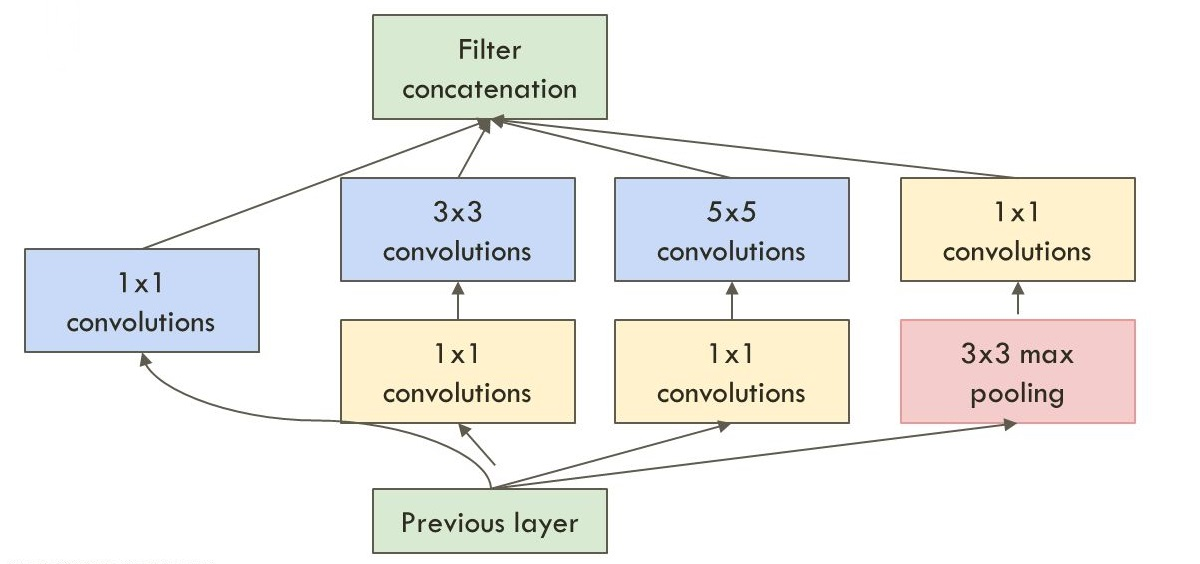
\includegraphics[width=0.8\linewidth]{concat.jpg} \caption{Συνένωση των εξόδων των φίλτρων στο επίπεδο Συνένωσης}
\label{figure:concat}  
\end{figure}


\subsubsection{Συνάρτηση Ενεργοποίησης(Activation Function) }
\label{subsubsec:3.1.3.6}


H συνάρτηση ενεργοποίησης αποφασίζει αν ένας νευρώνας πρέπει να ενεργοποιηθεί ή όχι. Σκοπός της συνάρτησης ενεργοποίησης είναι να εισάγει μη γραμμικότητα στη έξοδο ενός νευρώνα. Δύο από τις πιο συνηθισμένες συναρτήσεις ενεργοποίησης, που αναφέρθηκαν και πιο πάνω στα ANN, είναι η συνάρτηση Ανόρθωσης και η Σιγμοειδής συνάρτηση, οι οποίες παρουσιάζονται στις εικόνες \ref{figure:relu}, \ref{figure:sigmoid}. 





\begin{figure}[!h]
    \centering
      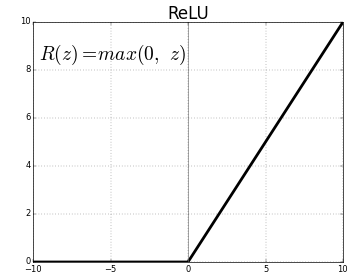
\includegraphics[width=0.5\linewidth]{relu.png} \caption{Συνάρτηση Ανόρθωσης}
      \label{figure:relu}    
  \end{figure}


\begin{figure}[!h]
    \centering
      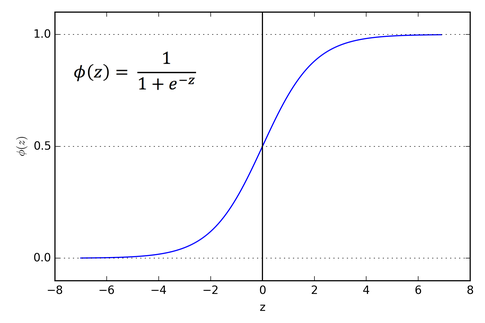
\includegraphics[width=0.5\linewidth]{sigmoid.png} \caption{Σιγμοειδής Συνάρτηση}
      \label{figure:sigmoid}    
  \end{figure}
  
\subsubsection{Επίπεδο Απόσυρσης(Dropout)}
\label{subsubsec:3.1.3.7}

Είναι μία τεχνική με σκοπό την μείωση της υπερεκπαίδευσης στα νευρωνικά δίκτυα. Υπερεκπαίδευση συμβαίνει όταν κατά τη διάρκεια της εκπαίδευσης το μοντέλο αποστηθίζει το σύνολο εκπαίδευσης με αποτέλεσμα να μην μπορεί να γενικεύσει. Έτσι, το μοντέλο αδυνατεί να προβλέψει σωστά την έξοδο για νέες εισόδους.
Κατά την εφαρμογή του επιπέδου Απόσυρσης, αγνοείται προσωρινά και με τυχαίο τρόπο κάποιο ποσοστό νευρώνων/φίλτρων τα οποία παράγουν μηδενική έξοδο και οι παράμετροι τους δεν ενημερώνονται. Το επίπεδο απόσυρσης εφαρμόζεται μόνο κατά τη διάρκεια της εκπαίδευσης. Έτσι, κατά τη διάρκεια της εκπαίδευσης, για κάθε επίπεδο που εφαρμόζεται απόσυρση, για κάθε είσοδο και για κάθε εποχή αγνοούνται κατά τυχαίο τρόπο κάποιο νευρώνες/φίλτρα. Στην εικόνα \ref{figure:dropout} παρουσιάζεται ένα πλήρες συνδεδεμένο δίκτυο χωρίς απόσυρση και το αντίστοιχο δίκτυο μετά την εφαρμογή απόσυρσης.


\begin{figure}[!h]
    \centering
      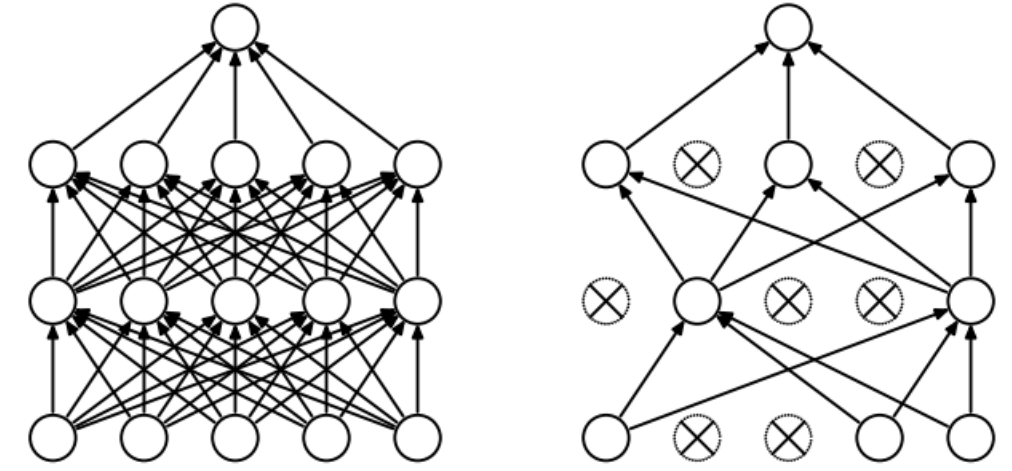
\includegraphics[width=0.8\linewidth]{dropout.png} \caption{Πλήρες συνδεδομένο δίκτυο χωρίς Dropout(αριστερά), με dropout(δεξιά)}
      \label{figure:dropout}    
  \end{figure}


\subsubsection{Κανονικοποίηση σε Πακέτα(Batch Normalization)}
\label{subsubsec:3.1.3.8}

Είναι μία τεχνική για βελτίωση της ταχύτητας, της επίδοσης και της σταθερότητας των CNN.\cite{BN}. Κατά τη διάρκεια της εκπαίδευσης ενός CNN, καθώς μεταβάλλονται οι παράμετροι των προηγούμενων επιπέδων, η κατανομή των εισόδων του τρέχοντος επιπέδου αλλάζει ανάλογα. Έτσι, το τρέχον επίπεδο πρέπει να αναπροσαρμόζεται συνεχώς σε νέες κατανομές. Ειδικότερα σε δίκτυα με πολλά επίπεδα το παραπάνω πρόβλημα είναι ακόμα πιο σοβαρό καθώς μικρές αλλαγές της κατανομής στα πρώτα επίπεδα θα ενισχυθούν καθώς διαδίδονται μέσα στο δίκτυο. Για τη μείωση αυτών των ανεπιθύμητων αλλαγών στις εισόδους κατά τη διάρκεια της εκπαίδευσης χρησιμοποιείται η κανονικοποίηση σε πακέτα. Η κανονικοποίηση δεν υφίσταται σε όλο το σύνολο δεδομένων αλλά σε μικρά υποσύνολα που ονομάζονται πακέτα. Επιπλέον, η τεχνική κανονικοποίησης σε πακέτα επιτρέπει τη χρήση υψηλότερου ρυθμού εκμάθησης(learning rate) ενώ συγχρόνως ρυθμίζει το δίκτυο έτσι ώστε να είναι ευκολότερη η γενίκευση και επομένως να μην είναι απαραίτητο να χρησιμοποιηθεί η τεχνική Απόσυρσης(dropout) για τη μείωση της υπερεκπαίδευσης.



Παρακάτω παρουσιάζονται τα βήματα που ακολουθούνται για τον υπολογισμό των νέων τιμών των εισόδων. Οι τιμές $\gamma$ και $\beta$ προσαρμόζονται από το δίκτυο κατά την διάρκεια της εκπαίδευσης.
 
 
\begin{algorithm}\captionsetup{labelfont={sc,bf}, labelsep=newline}
  \caption{Κανονικοποίηση σε πακέτα}\label{alg:the_alg}

\begin{algorithmic}

\State $Β \gets (x_{1},...x_{m})$

\State $μ_{Β}\gets \frac{1}{m}\sum_{i=1}^{m} x_{i} $

\State $σ_{Β}^2\gets \frac{1}{m} \sum_{i=1}^{m} (x_{i}- μ_{Β})^2$

\State $\hat{x_{i}} \gets \frac{x_{i}-μ_{Β}}{\sqrt(σ_{Β}^2 + ε)}$

\State $y_{i} \gets \gamma \hat{x_{i}} + \beta  \equiv BN_{\gamma, \beta}(x_{i}) $

\State return $y_{i}$
\end{algorithmic}
\end{algorithm}





\subsection{Support Vector Machine(SVM)}
\label{subsec:3.1.4}

To Support Vector Machine(SVM) είναι ένα μοντέλο για προβλήματα ταξινόμησης και παλινδρόμησης. \cite{svm} Μπορεί να λύσει τόσο  γραμμικά όσο και μη γραμμικά  προβλήματα. Ο αλγόριθμος δημιουργεί μία γραμμή ή ένα υπερεπίπεδο που χωρίζει τα δεδομένα στις επιθυμητές κλάσεις. Η δυσκολία του αλγορίθμου έγκειται στην εύρεση της βέλτιστης γραμμής ή υπερεπιπέδου για τη διαχωρισμό των δεδομένων.  

Στην \ref{figure:svm} οι κόκκινες και μπλε κουκίδες αναπαριστούν το σύνολο εκπαίδευσης ενώ τα X1 και X2 αποτελούν τα χαρακτηριστικά που περιγράφουν τα δεδομένα. Οι μπλε κουκίδες ανήκουν στην κλάση -1 ενώ οι κόκκινες στην κλάση +1. Να σημειωθεί ότι ενώ στην εικόνα \ref{figure:svm} τα δεδομένα περιγράφονται με δύο χαρακτηριστικά, στην πραγματικότητα τα δεδομένα συνήθως περιγράφονται από πολύ μεγαλύτερο αριθμό χαρακτηριστικών. Στην περίπτωση της παρούσας διπλωματικής τα χαρακτηριστικά των δεδομένων τα οποία εξάγονται από το πρώτο πλήρη συνδεδεμένο επίπεδο του νευρωνικού είναι 2048 ωστόσο μία τέτοια αναπαράσταση θα ήταν αδύνατη. Για ευκολότερη κατανόηση και μεγαλύτερη παραστατικότητα η παρακάτω ανάλυση του προβλήματος θα περιοριστεί σε προβλήματα δυαδικής ταξινόμησης δηλαδή διαχωρισμό των δεδομένων σε 2 κλάσεις.



\begin{figure}[!h]
    \centering
      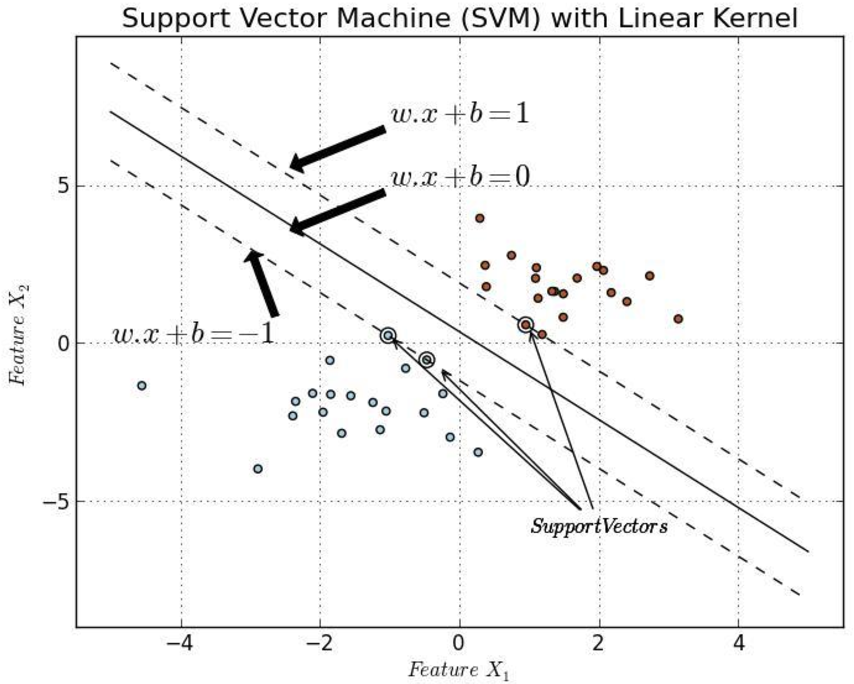
\includegraphics[width=0.8\linewidth]{svm2.png} \caption{Linear SVM}
\label{figure:svm}  
\end{figure}


Συνοπτικά, το πρόβλημα εύρεσης του βέλτιστου διαχωρισμού των δεδομένων μπορεί να τεθεί ως εξής. Έστω ένα σύνολο δεδομένων γραμμικά διαχωρίσιμο που κάθε δεδομένο ανήκει σε μία από τις δύο κλάσεις. Ο στόχος του αλγορίθμου είναι να μπορεί να  προβλέπει για νέα δεδομένα σε ποια κλάση ανήκουν. Αν θεωρήσουμε τα δεδομένα ως p-διαστατα διανύσματα, για το διαχωρισμό των δεδομένων πρέπει να βρεθεί ένα p-1 διαστατο υπερεπίπεδο. Για παράδειγμα για 2-διαστατα δεδομένα, αρκεί μία γραμμή για το διαχωρισμό τους ενώ για 3-διάστατα δεδομένα απαιτείται ένα επίπεδο(2D). Υπάρχουν πολλά υπερεπίπεδα που μπορούν να διαχωρίσουν τα δεδομένα ωστόσο ως βέλτιστο επιλέγεται το υπερεπίπεδο με το μεγαλύτερο περιθώριο μεταξύ των 2 κλάσεων. Έτσι, επιλέγεται το υπερεπίπεδο που η απόσταση από το πλησιέστερο δεδομένο κάθε κλάσης είναι μέγιστη. Αν αυτό το υπερεπιπεδο υπάρχει ονομάζεται\textit{ υπερεπίπεδο μέγιστου περιθωρίου} και ο γραμμικός ταξινομητής \textit{ταξινομητης μέγιστου περιθωρίου}. 



Αν το παραπάνω σύνολο  δεδομένων περιγραφεί  με σημεία της μορφής $(\vec{x}_{\,1},y_{1}),...,(\vec{x}_{\,n},y_{n})$, όπου τα $y_{i}$ είναι -1 ή 1 ανάλογα σε ποια κλάση ανήκουν τα $\vec{x}_{\,i}$ και τα $\vec{x}_{\,i}$ p-διάστατο διάνυσμα. Η περιοχή ανάμεσα στις δύο κλάσεις οριοθετείται από δύο υπερεπίπεδα και το  υπερεπιπεδο μεγίστου περιθωρίου που περιγράφηκε παραπάνω  βρίσκεται ανάμεσα στα δύο αυτά υπερεπίπεδα. Με ένα κανονικοποιημένο σύνολο δεδομένων, αυτά τα υπερεπίπεδα μπορούν να περιγραφούν με τις εξισώσεις \ref{eq:plane1}, \ref{eq:plane2}. Για την εξίσωση \ref{eq:plane1}, οτιδήποτε πάνω στο υπερεπίπεδο ή πάνω από το υπερεπίπεδο ανήκει στη κλάση 1 ενώ για την \ref{eq:plane2} οτιδήποτε πάνω στο υπερεπίπεδο ή κάτω από το υπερεπίπεδο ανήκει στη κλάση -1. 


\begin{equation} \label{eq:plane1}
\vec{w} \cdot  \vec{x} - b = 1
\end{equation}



\begin{equation} \label{eq:plane2}
\vec{w} \cdot  \vec{x} - b = -1
\end{equation}


Γεωμετρικά η απόσταση μεταξύ των δύο παραπάνω υπερεπιπέδων είναι $\frac{2}{||\vec{w}||}$. Επομένως, για να μεγιστοποιηθεί η απόσταση μεταξύ των υπερεπιπέδων, πρέπει να ελαχιστοποιηθεί το $||\vec{w}||$. Επιπλέον, πρέπει να ληφθούν υπόψη οι περιορισμοί \ref{eq:eq1} και \ref{eq:eq2}, ώστε τα δεδομένα  να μην βρίσκονται μέσα στο περιθώριο.


\begin{equation} \label{eq:eq1}
\vec{w}\cdot \vec{x}_{\,i} - b >= 1, ~αν ~y_{i} = 1
\end{equation}


\begin{equation} \label{eq:eq2}
\vec{w} \cdot \vec{x}_{\,i} - b <= 1, ~αν ~y_{i} = -1
\end{equation}
\\
\\
Τελικά, το πρόβλημα μπορεί να περιγραφεί ως εξής:


\begin{equation} \label{eq:eq3}
Minimize~||\vec{w}|| ~ for ~ y_{i}(\vec{w}\cdot \vec{x}_{\,i} - b)>= 1 για ~ i = 1,...,n
\end{equation}
\\


Μέσω της \ref{eq:eq3} υπολογίζονται τα $\vec{w}$ και $b$ τα οποία αρκούν για την περιγραφή του ταξινομητή. Η παραπάνω ανάλυση περιγράφει τη βασική λογική του αλγορίθμου, ωστόσο όταν τα δεδομένα δεν είναι γραμμικά διαχωρίσιμα, δηλαδή δεν μπορούν να διαχωριστούν από ένα υπερεπίπεδο, κάποια δεδομένα θα ταξινομούνται λάθος. Για αυτές τις περιπτώσεις ορίζεται μία επέκταση του SVM. Για την περιγραφή του νέου προβλήματος γίνεται χρήση της συνάρτησης hinge loss:
\\


\begin{equation} \label{eq:eq4}
max(0,1-y_{i}(\vec{w} \cdot \vec{x}_{\,i} - b))
\end{equation}
όπου η $ y_{i}$ είναι η πραγματική κλάση που ανήκει το $\vec{x_{\,i}}$ και $\vec{w} \cdot \vec{x}_{\,i}-b$ είναι η έξοδος του αλγορίθμου για το $\vec{x_{\,i}}$.


Η συνάρτηση είναι $0$, αν το $\vec{x_{\,i}}$ έχει ταξινομηθεί στη σωστή κλάση καθώς ο όρος $y_{i}(\vec{w}*\vec{x}_{\,i}-b)$ είναι πάντα μεγαλύτερος ή ίσος του 1 για σωστή ταξινόμηση του $\vec{x_{\,i}}$ οπότε το $1-y_{i}(\vec{w} \cdot \vec{x}_{\,i}-b)$ θα παίρνει τιμές μικρότερες ή ίσες το μηδενός. Ενώ όταν το $\vec{x_{\,i}}$ ταξινομηθεί σε λάθος κλάση, δηλαδή βρεθεί στη λάθος πλευρά του περιθωρίου,
 ο όρος $1-y_{i}(\vec{w} \cdot \vec{x}_{\,i}-b)$ θα παίρνει θετικές τιμές ανάλογες της απόστασης από το περιθώριο. Το πρόβλημα ελαχιστοποίησης  αναδιατυπώνεται ως εξής:


\begin{equation} \label{eq:eq5}
\frac{1}{n}  \sum_{i=1}^{n} max(0,1-y_{i}(\vec{w} \cdot \vec{x}_{\,i} - b))] + \lambda \cdot  ||\vec{w}||^2
\end{equation}
όπου η παράμετρος λ ορίζει το συμβιβασμό μεταξύ αύξησης περιθωρίου με παράλληλη μείωση των σωστών ταξινομήσεων.



Στην παρούσα διπλωματική εκτός του γραμμικού ταξινομητή, χρησιμοποιείται και ένας μη γραμμικός ταξινομητής με συνάρτηση πυρήνα την Gaussian Radial Basis η οποία περιγράφεται από την εξίσωση \ref{eq:eq7}. Για τη χρήση μη γραμμικών ταξινομητών ο  SVM χρησιμοποιεί μια συνάρτηση πυρήνα για να απεικονίσει το σύνολο δεδομένων σε ένα υψηλότερης διάστασης χώρο με σκοπό να γίνει γραμμικό σύνολο δεδομένων.


\begin{equation} \label{eq:eq7}
k(\vec{x}_{\,i},\vec{x}_{\,j}) = \exp(-\gamma ||\vec{x}_{\,i}- \vec{x}_{\,j} ||^2) ~ για ~ \gamma>0
\end{equation}



\section{Inception V3}
\label{sec:3.2}


Το Inception V3\cite{Szegedy} το οποίο χρησιμοποιήθηκε στην παρούσα διπλωματική αποτελεί ένα ευρέως χρησιμοποιούμενο συνελικτικό δίκτυο. Η αρχιτεκτονική Inception στην οποία ανήκει και το νευρωνικό Inception V3 αποτελείται από τις εξής εκδόσεις: Inception V1, Inception V2, Inception V3,Inception v4 και Inception-ResNet. Κάθε επόμενη έκδοση περιέχει βελτιώσεις στην επίδοση και στην ακρίβεια σε σχέση με την προηγούμενη. Ωστόσο, είναι δυνατόν μία παλαιότερη έκδοση να επιφέρει καλύτερα αποτελέσματα σε ένα  συγκεκριμένο σύνολο δεδομένων, σε σχέση με μία πιο καινούρια.


Η αρχιτεκτονική Inception αποτελεί ορόσημο για την ανάπτυξη των συνελικτικών δικτύων. Πριν από αυτή, τα πιο αποτελεσματικά CNN αύξαναν τα συνελικτικά επίπεδα πηγαίνοντας σε όλο και σε πιο βαθιες αρχιτεκτονικές, επιδιώκοντας καλύτερη επίδοση.


Στην αρχιτεκτονική Inception δεν ακολουθήθηκε η ίδια λογική, δηλαδή προσθήκη όλο και περισσότερων συνελικτικών επιπέδων αλλά προτάθηκε μία αρκετά πιο περίπλοκη δομή η οποία είναι αποτέλεσμα ιδεών που αναπτύχθηκαν από πολλούς ερευνητές κατά τη διάρκεια των προηγούμενων ετών.
Στην εικόνας \ref{figure:incV32} αποτυπώνεται η δομή του νευρωνικού Inception V3.


\begin{figure}[!h]

    \centering
      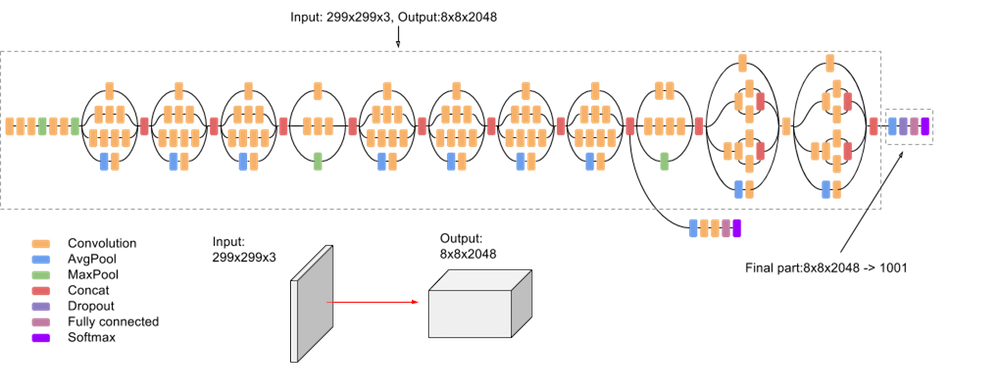
\includegraphics[width=1\linewidth]{incV3_2.png} \caption{Αρχιτεκτονική του νευρωνικού Inception V3}      
      \label{figure:incV32}  

  \end{figure}
  
  
\subsection{Τεχνικές σχεδίασης Inception V3}
\label{subsec:3.3.2}
Παρακάτω θα παρουσιαστούν οι κυριότερες τεχνικές σχεδίασης που προτάθηκαν στο Inception V3, ως μία βελτίωση των προηγούμενων εκδόσεων.


\subsubsection{Παραγοντοποίηση σε μικρότερα συνελικτικά επίπεδα}
\label{subsubsec:3.3.2.1}
Συνελίξεις με μεγαλύτερα χωρικά φίλτρα(πχ $5x5$ ή $7x7$) τείνουν να είναι δυσανάλογα ακριβές στους υπολογισμούς. Ένα συνελικτικό επίπεδο $5x5$ είναι 2.78 φορές πιο ακριβό υπολογιστικά σε σχέση με ένα $3x3$, με τον ίδιο αριθμό φίλτρων. Ωστόσο, στο $5x5$ συνελικτικό επίπεδο παρέχει μεγαλύτερη εκφραστικότητα. Για να είναι δυνατή η μείωση των παραμέτρων χωρίς όμως μείωση της ακρίβειας, προτείνεται η αντικατάσταση του φίλτρου $5x5$, χρησιμοποιώντας δύο συνελικτικα επίπεδα με $3x3$ φίλτρα και ίδιο αριθμό φίλτρων. Σε αυτή την περίπτωση ο αριθμός των παραμέτρων μειώνεται κατά $\frac{9+9}{25} = 28\%$. Στην εικόνα \ref{figure:a1} παρουσιάζεται ένα τμήμα του δικτύου, πριν και μετά την αντικατάσταση. Η παραπάνω αντικατάσταση μπορεί να γενικευθεί και για φίλτρα μεγαλύτερων διαστάσεων από $5x5$ , με αντικατάσταση αντίστοιχων $3x3$ επιπέδων.


\begin{figure}[!h]
\centering
\begin{subfigure}{.5\textwidth}
  \centering
  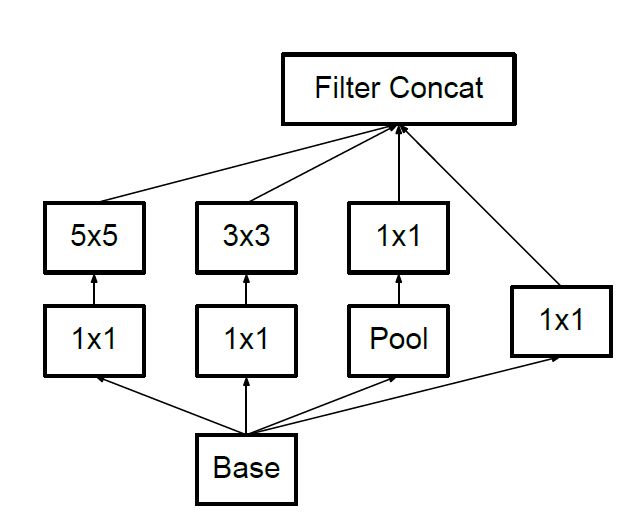
\includegraphics[scale=0.5]{0incV3.PNG}
  \caption{Αρχική δομή}
  \label{fig:sub11}
\end{subfigure}
\begin{subfigure}{.5\textwidth}
  \centering
  \includegraphics[scale=0.5]{1incV3.PNG}
  \caption{Μετά την αντικατάσταση}
  \label{fig:sub21}
\end{subfigure}
\caption{Αντικατάσταση του επιπέδου 5x5, με δύο 3x3 επίπεδα}
\label{figure:a1}
\end{figure}



\subsubsection{Παραγοντοποίηση σε μικρότερα μη συμμετρικά συνελικτικά επίπεδα}
\label{subsubsec:3.3.2.2}
Όπως παρουσιάστηκε και στην προηγούμενη παράγραφο ένα επίπεδο με φίλτρα μεγαλύτερων από $3x3$ διαστάσεων, μπορούν να αντικατασταθούν με μία  
αλληλουχία  επιπέδων με φίλτρα διαστάσεων $3x3$ και ίδιο αριθμό φίλτρων. Ωστόσο, τίθεται το ερώτημα, αν τα φίλτρα $3x3$ μπορούν να παραγοντοποιηθούν σε περισσότερα επίπεδα με μικρότερες διαστάσεις φίλτρων. Μία σκέψη θα ήταν να μετατραπούν σε δύο επίπεδα με $2x2$ φίλτρα, ωστόσο όπως αποδείχθηκε πειραματικά η παραγοντοποίηση σε ασύμμετρες συνελίξεις μπορεί να επιφέρει καλύτερα αποτελέσματα ενώ συγχρόνως επιφέρει μεγαλύτερη μείωση των παραμέτρων. Για παράδειγμα, έστω, φίλτρο διαστάσεων 3x3. Συνολικά, για αυτό το φίλτρο θα είχαμε $3*3 = 9$ παραμέτρους. Έστω τώρα ότι γίνεται αντικατάσταση του φίλτρο 3x3, με δύο φίλτρα  διαστάσεων 3x1 και 1x3. Συνολικά, τα 2 φίλτρα έχουν $3*1 + 1*3 = 6$ παραμέτρους. Ο αριθμός των παραμέτρων μειώθηκε κατά $33\%$. Αν αντίθετα, προτιμούνταν η χρήση $2$ συλλεκτικών επιπέδων με διάσταση φίλτρων $2x2$ τότε οι παράμετροι θα μειωνόταν κατά $\frac{2(2+2)}{3 \cdot 3}= 11\%$. Γενικά, η παραπάνω ανάλυση μπορεί να γενικευθεί για $nxn$ φίλτρα με αντικατάσταση από $1xn$ φίλτρα και $nx1$ φίλτρα. Στην εικόνα  \ref{figure:b2} παρουσιάζεται η παραπάνω αντικατάσταση.


\begin{figure}[!h]
\centering
\begin{subfigure}{.5\textwidth}
  \centering
  \includegraphics[scale=0.5]{1incV3.PNG}
  \caption{Αρχική δομή}
  \label{fig:sub1b2}
\end{subfigure}
\begin{subfigure}{.5\textwidth}
  \centering
  \includegraphics[scale=0.5]{2incV3.PNG}
  \caption{Μετά την αντικατάσταση}
  \label{fig:sub2b2}
\end{subfigure}
\caption{Αντικατάσταση κάθε επιπέδου 3x3, με ένα επίπεδο 1xn και ένα nx1}
\label{figure:b2}
\end{figure}


\subsubsection{Βοηθητικός Ταξινομητης}
\label{subsubsec:3.3.2.3}
Σε αντίθεση με προηγούμενες εκδόσεις της αρχιτεκτονικής Inception που χρησιμοποιήθηκαν 2 βοηθητικοί ταξινομητές στο Inception V3 χρησιμοποιήθηκε ένας μόνο βοηθητικός ταξινομητής στο τελευταίο $17x17$ συνελικτικό επίπεδο. Σε σχέση με τις προηγούμενες εκδόσεις που ο σκοπός των βοηθητικών ταξινομητών ήταν να επιτρέψουν πιο μεγάλο βάθος στο δίκτυα, ο σκοπός του βοηθητικού ταξινομητή στο Inception V3 είναι η χρήση του ως ρυθμιστή(regularizer) του δικτύου. Για την παρούσα διπλωματική παραλήφθηκε ο βοηθητικός ταξινομητής.


\subsubsection{Αποτελεσματική μείωση των διαστάσεων των χαρτών χαρακτηριστικών}
\label{subsubsec:3.3.2.4}
Για τη μείωση των διαστάσεων των χαρτών χαρακτηριστικών συνήθως χρησιμοποιείται μια συνάρτηση υποδειγματοληψίας. Επιπλέον, πριν την εφαρμογή του επιπέδου υποδειγματοληψίας τα κανάλια των χαρτών χαρακτηριστικών συχνά αυξάνονται με την εφαρμογή ενός συνελικτικού επιπέδου. 


Οπότε για να μειώσουμε τις διαστάσεις των χαρτών χαρακτηριστικών από k φίλτρα διαστάσεων dxd, σε $2k$ φίλτρα διαστάσεων $\frac{d}{2} x \frac{d}{2}$ πρέπει πρώτα να εφαρμοστεί ένα συνελικτικό επίπεδο με $2k$ φίλτρα και στη συνέχεια ένα επίπεδο υποδειγματοληψίας για την μείωση των διαστάσεων. Οι συνολικοί υπολογισμοί για τα παραπάνω είναι $2d^2 k^2$ και είναι ασύμφοροι λόγω της χρήσης συνελικτικού επιπέδου πριν τη μείωση των διαστάσεων. Αν γίνει αλλαγή στη σειρά του συνελικτικού επιπέδου και του επιπέδου υποδειγματοληψίας καταλήγουμε σε $\frac{d}{2}^2 k^2$, μειώνοντας το κόστος κατά $\frac{1}{4}$. Αυτός ο τρόπος δεν είναι ο πλέον αποδοτικός καθώς μειώνεται η διάσταση της αναπαράστασης σε $(d/2)^2 k$, καταλήγοντας σε μείωση της εκφραστικότητας του δικτύου. Αντί να γίνουν τα παραπάνω στο Inception V3 προτείνεται η χρήση δύο παράλληλων blocks: των P και C, το P είναι ένα επίπεδο υποδειγματοληψίας με παράθυρο $2x2$ και το C ένα συνελικτικό επίπεδο με ίδιο αριθμό φίλτρων με τον αρχικό χάρτη χαρακτηριστικών. Να σημειωθεί ότι το συνελεκτικό επίπεδο παράγεται με βήμα δύο, το οποίο σημαίνει ότι κατά τη συνέλιξη το φίλτρο θα μετατοπίζεται πάνω στην εικόνα, προσπερνώντας κάθε φορά ένα εικονοστοιχείο και πηγαίνοντας στο επόμενο. Στην εικόνα \ref{figure:PC} παρουσιάζονται γραφικά τα παραπάνω.



\begin{figure}[!h]
\centering
\begin{subfigure}{.5\textwidth}
  \centering
  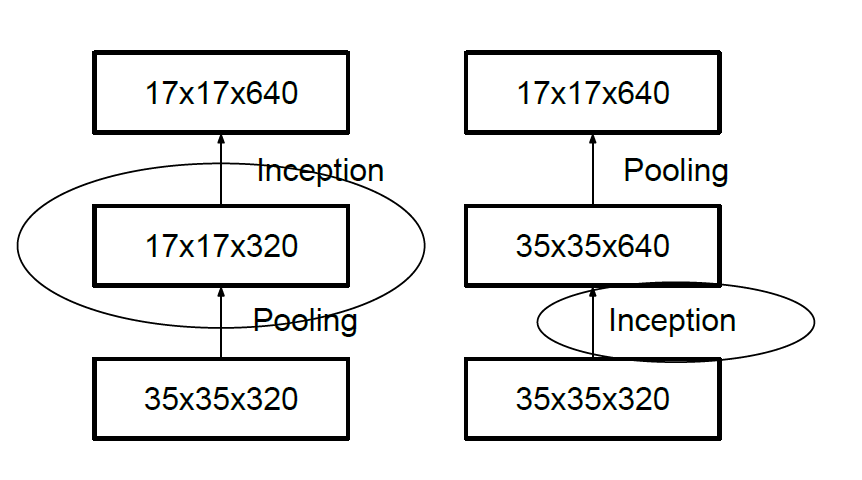
\includegraphics[scale=0.35]{expensive0incV3.PNG}
  \caption{Μη βέλτιστοι τρόποι μείωσης των διαστάσεων των χαρτών χαρακτηριστικών}
  \label{fig:sub1b}
\end{subfigure}%
\begin{subfigure}{.4\textwidth}
  \centering
  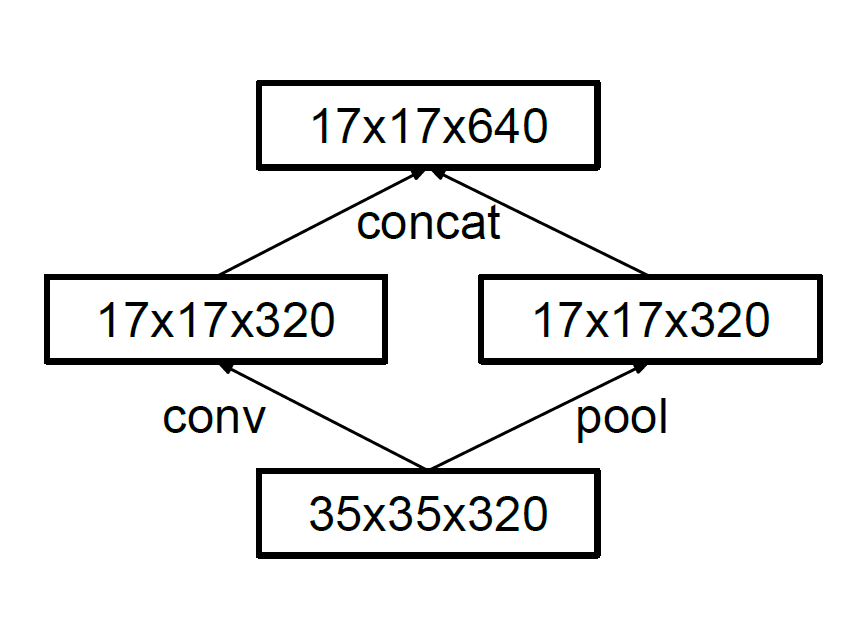
\includegraphics[scale=0.25]{3inv3.PNG}
  \caption{Βέλτιστος τρόπος μείωσης των διαστάσεων των χαρτών χαρακτηριστικών}
  \label{fig:sub2b}
\end{subfigure}
\caption{Μείωση των διαστάσεων των χαρτών Χαρακτηριστικών}
\label{figure:PC}
\end{figure}


\section{Εργαλεία}
\label{sec:3.4}
Το \textbf{matlab} είναι μία προγραμματιστική πλατφόρμα σχεδιασμένη ειδικά για μηχανικούς και ερευνητές με δυνατότητες ανάλυσης δεδομένων, ανάπτυξης αλγορίθμων, δημιουργίας μοντέλων και εφαρμογών. Στην παρούσα διπλωματική χρησιμοποιήθηκε κατά την διαδικασία επεξεργασίας των εικόνων, η οποία περιλαμβάνει την ανίχνευση του αμφιβληστροειδούς και τη μείωση των διαστάσεων των εικόνων.

Το \textbf{Tensorflow(TF)} είναι μία δωρεάν, ανοιχτού κώδικα βιβλιοθήκη, για μαθηματικούς υπολογισμούς. Χρησιμοποιείται σε πληθώρα εφαρμογών αλλά έχει καθιερωθεί για τη χρήση του σε Machine Learning εφαρμογές όπως Νευρωνικά Δίκτυα. Το TF μπορεί να τρέξει σε πολλαπλές CPUs και GPUs ενώ υποστηρίζει  64-bit Linux, mac OS, Windows, και πλατφόρμες κινητών όπως Android and iOS.


Το \textbf{Keras} είναι μία υψηλού επιπέδου βιβλιοθήκη νευρωνικών δικτύων γραμμένη σε Python. Μπορεί να τρέξει πάνω από TensorFlow, CNTK ή Theano.  Αναπτύχθηκε με γνώμονα τους γρήγορους υπολογισμούς και το γρήγορο πειραματισμό. Περιέχει υλοποιήσεις από αρκετά δομικά στοιχεία των νευρωνικών δικτύων. Επιπλέον, περιέχει έτοιμες υλοποιήσεις ευρέως διαδεδομένων νευρωνικών δικτύων.  Στην παρούσα διπλωματική επιλέχθηκε η χρήση της βιβλιοθήκης Keras πάνω σε Tensorflow για δημιουργία και εκπαίδευση των μοντέλων. Συνδυαστικά χρησιμοποιήθηκαν και άλλες πολλές βιβλιοθήκες της Python για διάφορους μετασχηματισμούς των εικόνων και για τη δημιουργία μοντέλων SVM.  



\thispagestyle{plain}
\chapter{Σύνολα Δεδομένων και Προεπεξεργασία Εικόνων}
\label{chap:4}
\section{Σύνολα Δεδομένων}
\label{sec:4.1}

\subsection{Σύνολο Δεδομένων Kaggle}
\label{subsec:4.1.1}
Τα δεδομένα προέρχονται από ένα διαγωνισμό του Κaggle που διεξήχθη το 2015 και αφορούσε την διάγνωση της Διαβητικής Αμφιβληστροειδοπάθειας\cite{Kaggle}. Στο διαγωνισμό ζητήθηκε η διάγνωση της σοβαρότητας της ασθένειας για αυτό χρησιμοποιήθηκαν μοντέλα για ταξινόμηση πολλών κλάσεων. Το σύνολο δεδομένων είναι χωρισμένο σε πέντε κλάσεις ως εξής: 0 - No, 1 - Mild, 2 -Moderate, 3 - Severe, 4 - Proliferative.

Το σύνολο δεδομένων Kaggle αποτελείται από εικόνες υψηλής ανάλυσης διαφόρων διαστάσεων (433x289 μέχρι 5184x3456), οι οποίες έχουν τραβηχτεί σε διάφορες συνθήκες φωτισμού και με διάφορα μοντέλα και τύπους κάμερας. Για κάθε ασθενή είναι διαθέσιμες εικόνες του αμφιβληστροειδούς και των δύο ματιών. Η αντιστοίχιση των εικόνων στις διάφορες κλάσεις έγινε από έναν κλινικό ιατρό.

To σύνολο εκπαίδευσης αποτελείται από 35126 εικόνες RGB, ενώ το σύνολο ελέγχου από 53576 εικόνες RGB. H κάθε εικόνα των παραπάνω συνόλων ανήκει σε μία από τις πέντε προαναφερθείσες κλάσεις. Τα δύο σύνολα ενώθηκαν και στη συνέχεια χωρίστηκαν εκ νέου στα σύνολα: εκπαίδευσης,  επικύρωσης και ελέγχου. Παρακάτω θα γίνει μία συνοπτική περιγραφή του διαχωρισμού του συνόλου δεδομένων ενώ για περισσότερη παραστατικότητα παρατίθεται η εικόνα \ref{figure:data}.
\begin{figure}[!h]
    \centering
      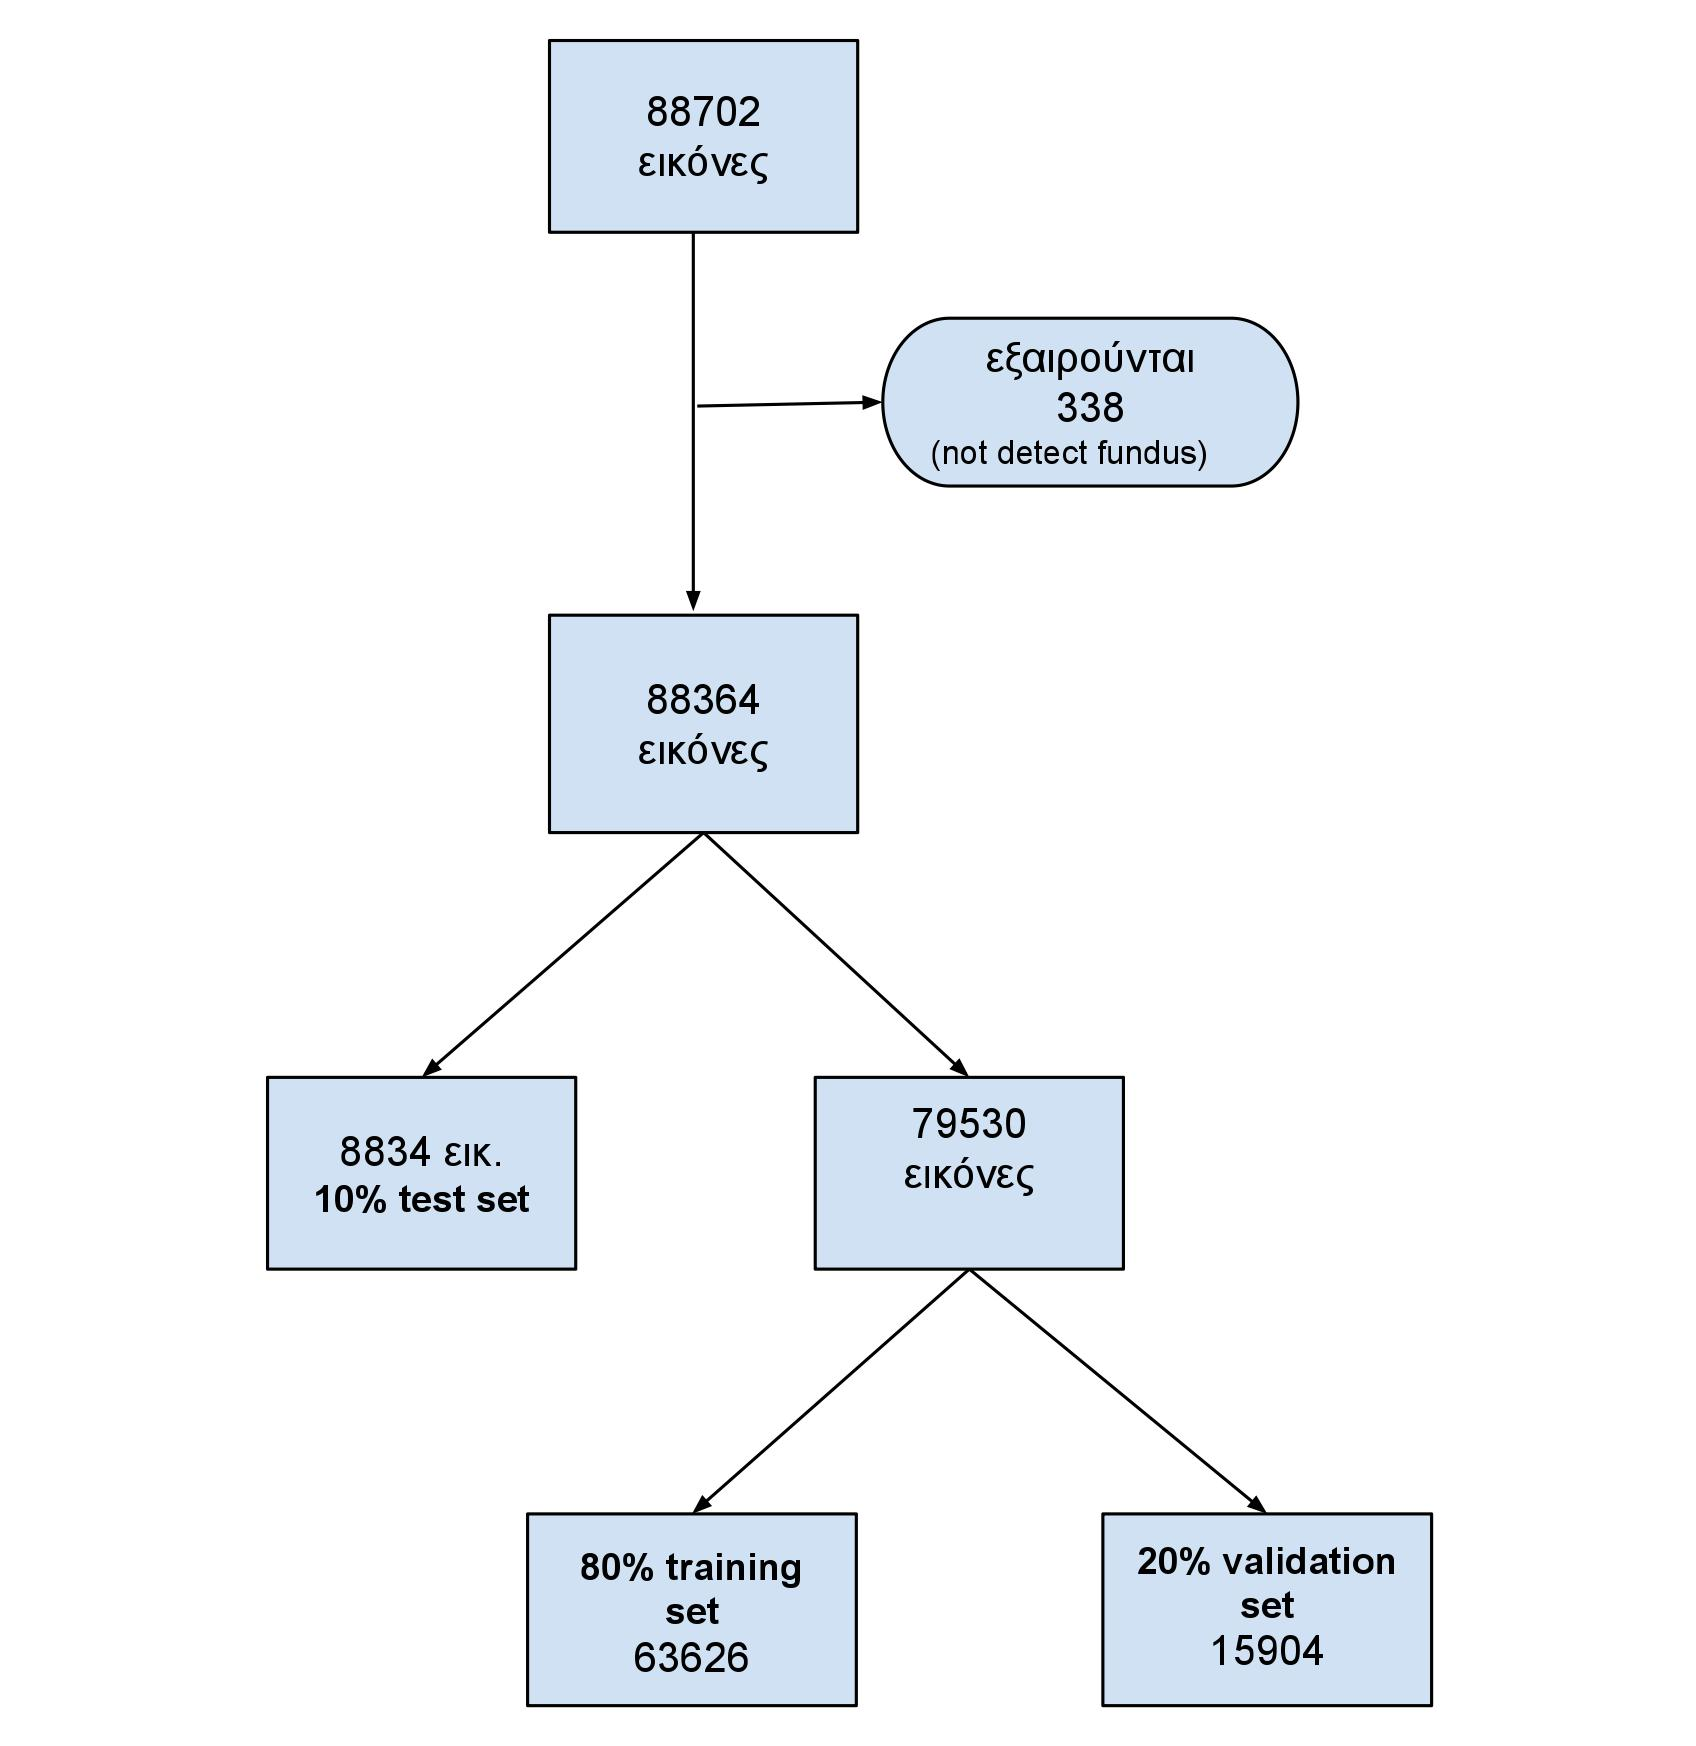
\includegraphics[width=0.9\linewidth]{data.jpg} \caption{ Διαχωρισμός του συνόλου δεδομένων στα σύνολα εκπαίδευσης, επικύρωσης και ελέγχου}
\label{figure:data}    
  \end{figure}

Αρχικά, το ενοποιημένο σύνολο αποτελείται από 88702 εικόνες και η κάθε εικόνα ανήκει σε μία από τις πέντε κλάσεις. Μετά την εφαρμογή του μετασχηματισμού Hough,  οι εικόνες στις οποίες δεν ανιχνεύεται ο αμφιβληστροειδής, εξαιρούνται. Οπότε καταλήγουμε με 88364 εικόνες. Στη συνέχεια, επιλέγουμε τυχαία $10\%$ των δεδομένων από κάθε κλάση για το σύνολο ελέγχου ενώ το υπόλοιπο $90\%$, διαχωρίζεται εκ νέου σε σύνολο εκπαίδευσης και σύνολο επικύρωσης με ποσοστά $80\%$ και $20\%$ από κάθε κλάση , αντίστοιχα.


Στο παραπάνω σύνολο δεδομένων υπάρχει θόρυβος ο οποίος οφείλεται στο γεγονός ότι η αντιστοίχιση των εικόνων στις κλάσεις έγινε μόνο από έναν κλινικό ιατρό και από την κακή ποιότητα ορισμένων εικόνων. Ορισμένες εικόνες έχουν τραβηχθεί σε συνθήκες χαμηλής ή υψηλης έκθεσης, κακής εστίασης ενώ σε ορισμένες περιπτώσεις υπάρχει αλλοίωση του περιεχομένου της εικόνας.

Μόλις το $75\%$ των εικόνων θεωρείται βαθμολογήσιμο.\cite{Rakhlin} Οι υπόλοιπες εικόνες παρουσιάζουν κακή ποιότητα. Στην εικόνα \ref{figure:badquality} παρατίθενται μερικά παραδείγματα εικόνων κακής ποιότητας.  
\begin{figure}[!h]
    \centering
      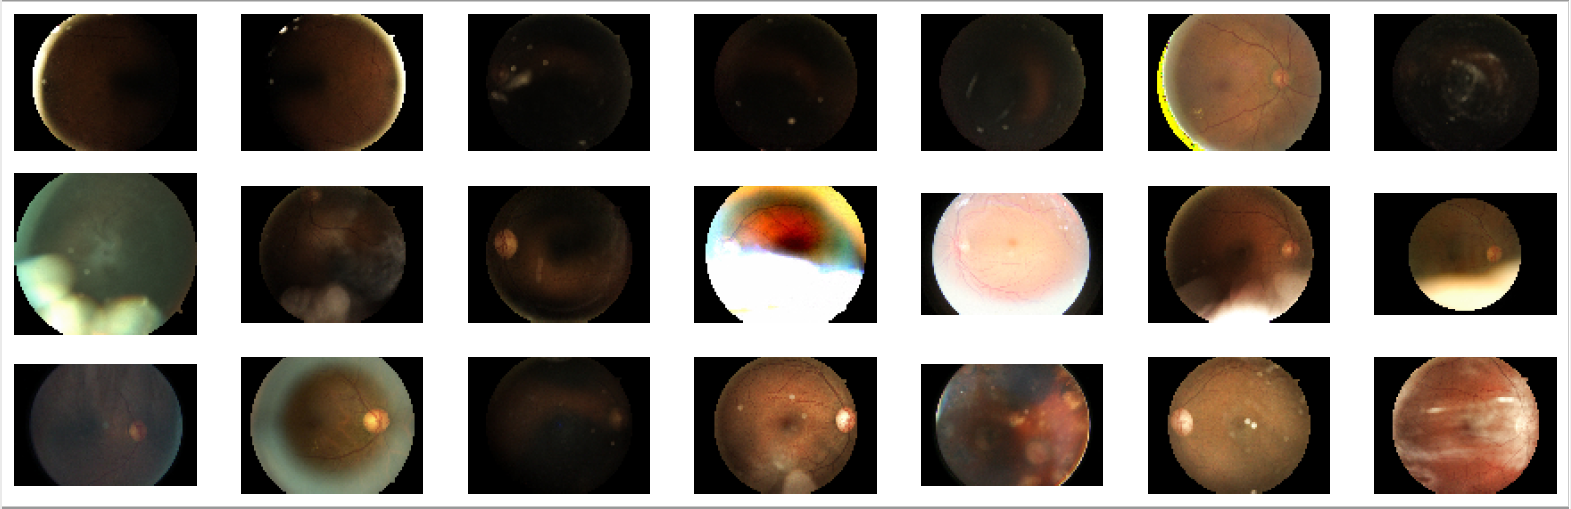
\includegraphics[width=1\linewidth]{badQuality.PNG} \caption{Εικόνες του συνόλου δεδομένων Kaggle που έχουν τραβηχτεί σε συνθήκες χαμηλής ή υψηλής έκθεσης, κακής εστίασης ενώ σε ορισμένες περιπτώσεις υπάρχει αλλοίωση του περιεχομένου της εικόνας}
 \label{figure:badquality}    
  \end{figure}


\subsection{Σύνολο Δεδομένων Messidor 2}
\label{subsec:4.1.2}
Το σύνολο δεδομένων Messidor 2 αποτελείται από 1748 εικόνες του αμφιβληστροειδούς. Η εικόνες έχουν ληφθεί με την κάμερα  Topcon TRC NW6 μη μυδριακής βάσης με οπτικό πεδίο 45 μοιρών και έχουν διαστάσεις 1440x960, 2240x1488 ή 2304x1536 εικονοστοιχεία. Αποτελεί μία επέκταση του συνόλου δεδομένων Messidor1\cite{Decencière}. Το Messidor2 χρησιμοποιήθηκε εξ ολοκλήρου ως ένα δεύτερο σύνολο ελέγχου.Στην εικόνα \ref{figure:mes}  παρουσιάζονται κάποια ενδεικτικά δείγματα του συνόλου δεδομένων Messidor 2.

\begin{figure}[!h]
    \centering
      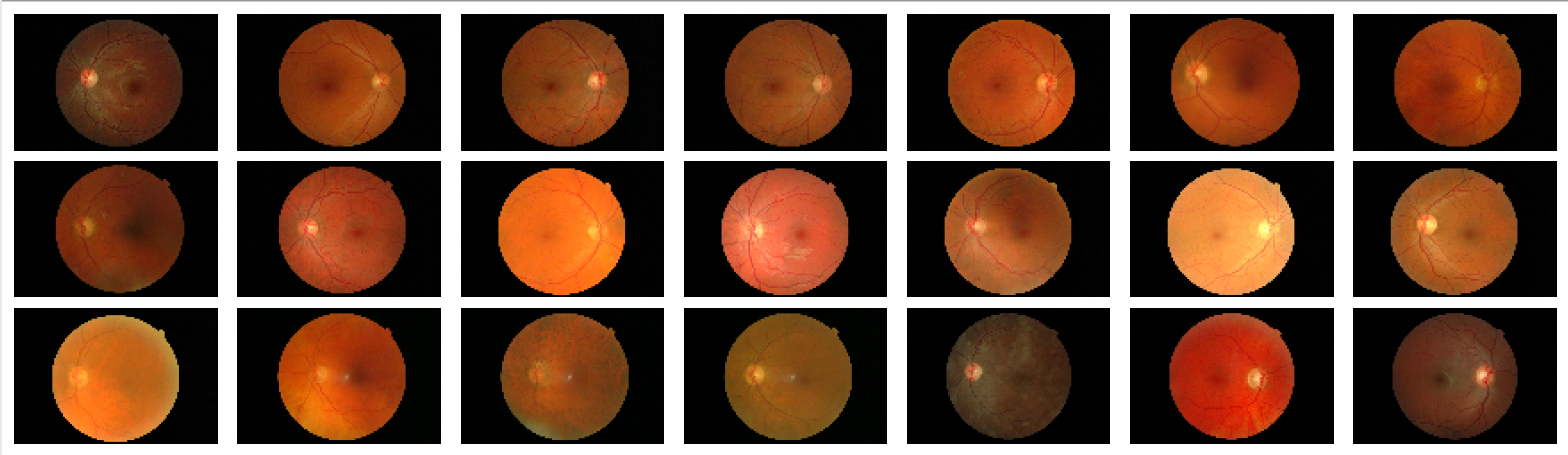
\includegraphics[width=1\linewidth]{mes3.PNG} \caption{Eνδεικτικά δείγματα του συνόλου δεδομένων Messidor 2}
\label{figure:mes}  
\end{figure}



\section{Προεπεξεργασία Εικόνων}
\label{sec:4.2}
\subsection{Διαδικασία Προεπεξεργασίας Εικόνων} 
\label{sec:4.2.1}
Για την επεξεργασία των εικόνων ακολουθείται η εξής διαδικασία. Αρχικά, μειώνονται οι διαστάσεις της εικόνας με σκοπό την ελάττωση του χρόνου επεξεργασίας, χωρίς ωστόσο να χαθεί η αναλογία. Στη συνέχεια εφαρμόζεται ο μετασχηματισμός Hough για την ανίχνευση του αμφιβληστροειδούς. Ο μετασχηματισμός Hough θα εξηγηθεί λεπτομερώς σε επόμενη παράγραφο. Επειδή, ο αλγόριθμος μπορεί να ανιχνεύσει πάνω από έναν κύκλους, η ακτίνα εύρεσης περιορίζεται στο διάστημα $[\frac{3mindim}{8},\frac{maxdim}{2}]$, όπου $mindim$ η μικρότερη διάσταση της εικόνας και $maxdim$ η μεγαλύτερη διάσταση της εικόνας. Το διάστημα αυτό υπολογίστηκε πειραματικά ώστε να καλύπτει όλες τις εικόνες. Επιπλέον, από τους κύκλους που ανιχνεύονται επιλέγεται ο πιο ισχυρός. Η επιλογή του πιο ισχυρού κύκλου σε συνδυασμό με τον περιορισμό του διαστήματος εύρεσης της ακτίνας, περιορίζει αρκετά το ενδεχόμενο λανθασμένης εύρεσης κύκλου. 

Το σύνολο δεδομένων Kaggle περιέχει δύο μορφές εικόνων, όπως μπορούμε να δούμε στην εικόνα \ref{figure:2morfes}. Η μία μορφή περιέχει ολόκληρο τον αμφιβληστροειδή ενώ η δεύτερη έχει κομμένο το πάνω και κάτω μέρος του αμφιβληστροειδούς.

\begin{figure}[!h]
\centering
\begin{subfigure}{.5\textwidth}
  \centering
  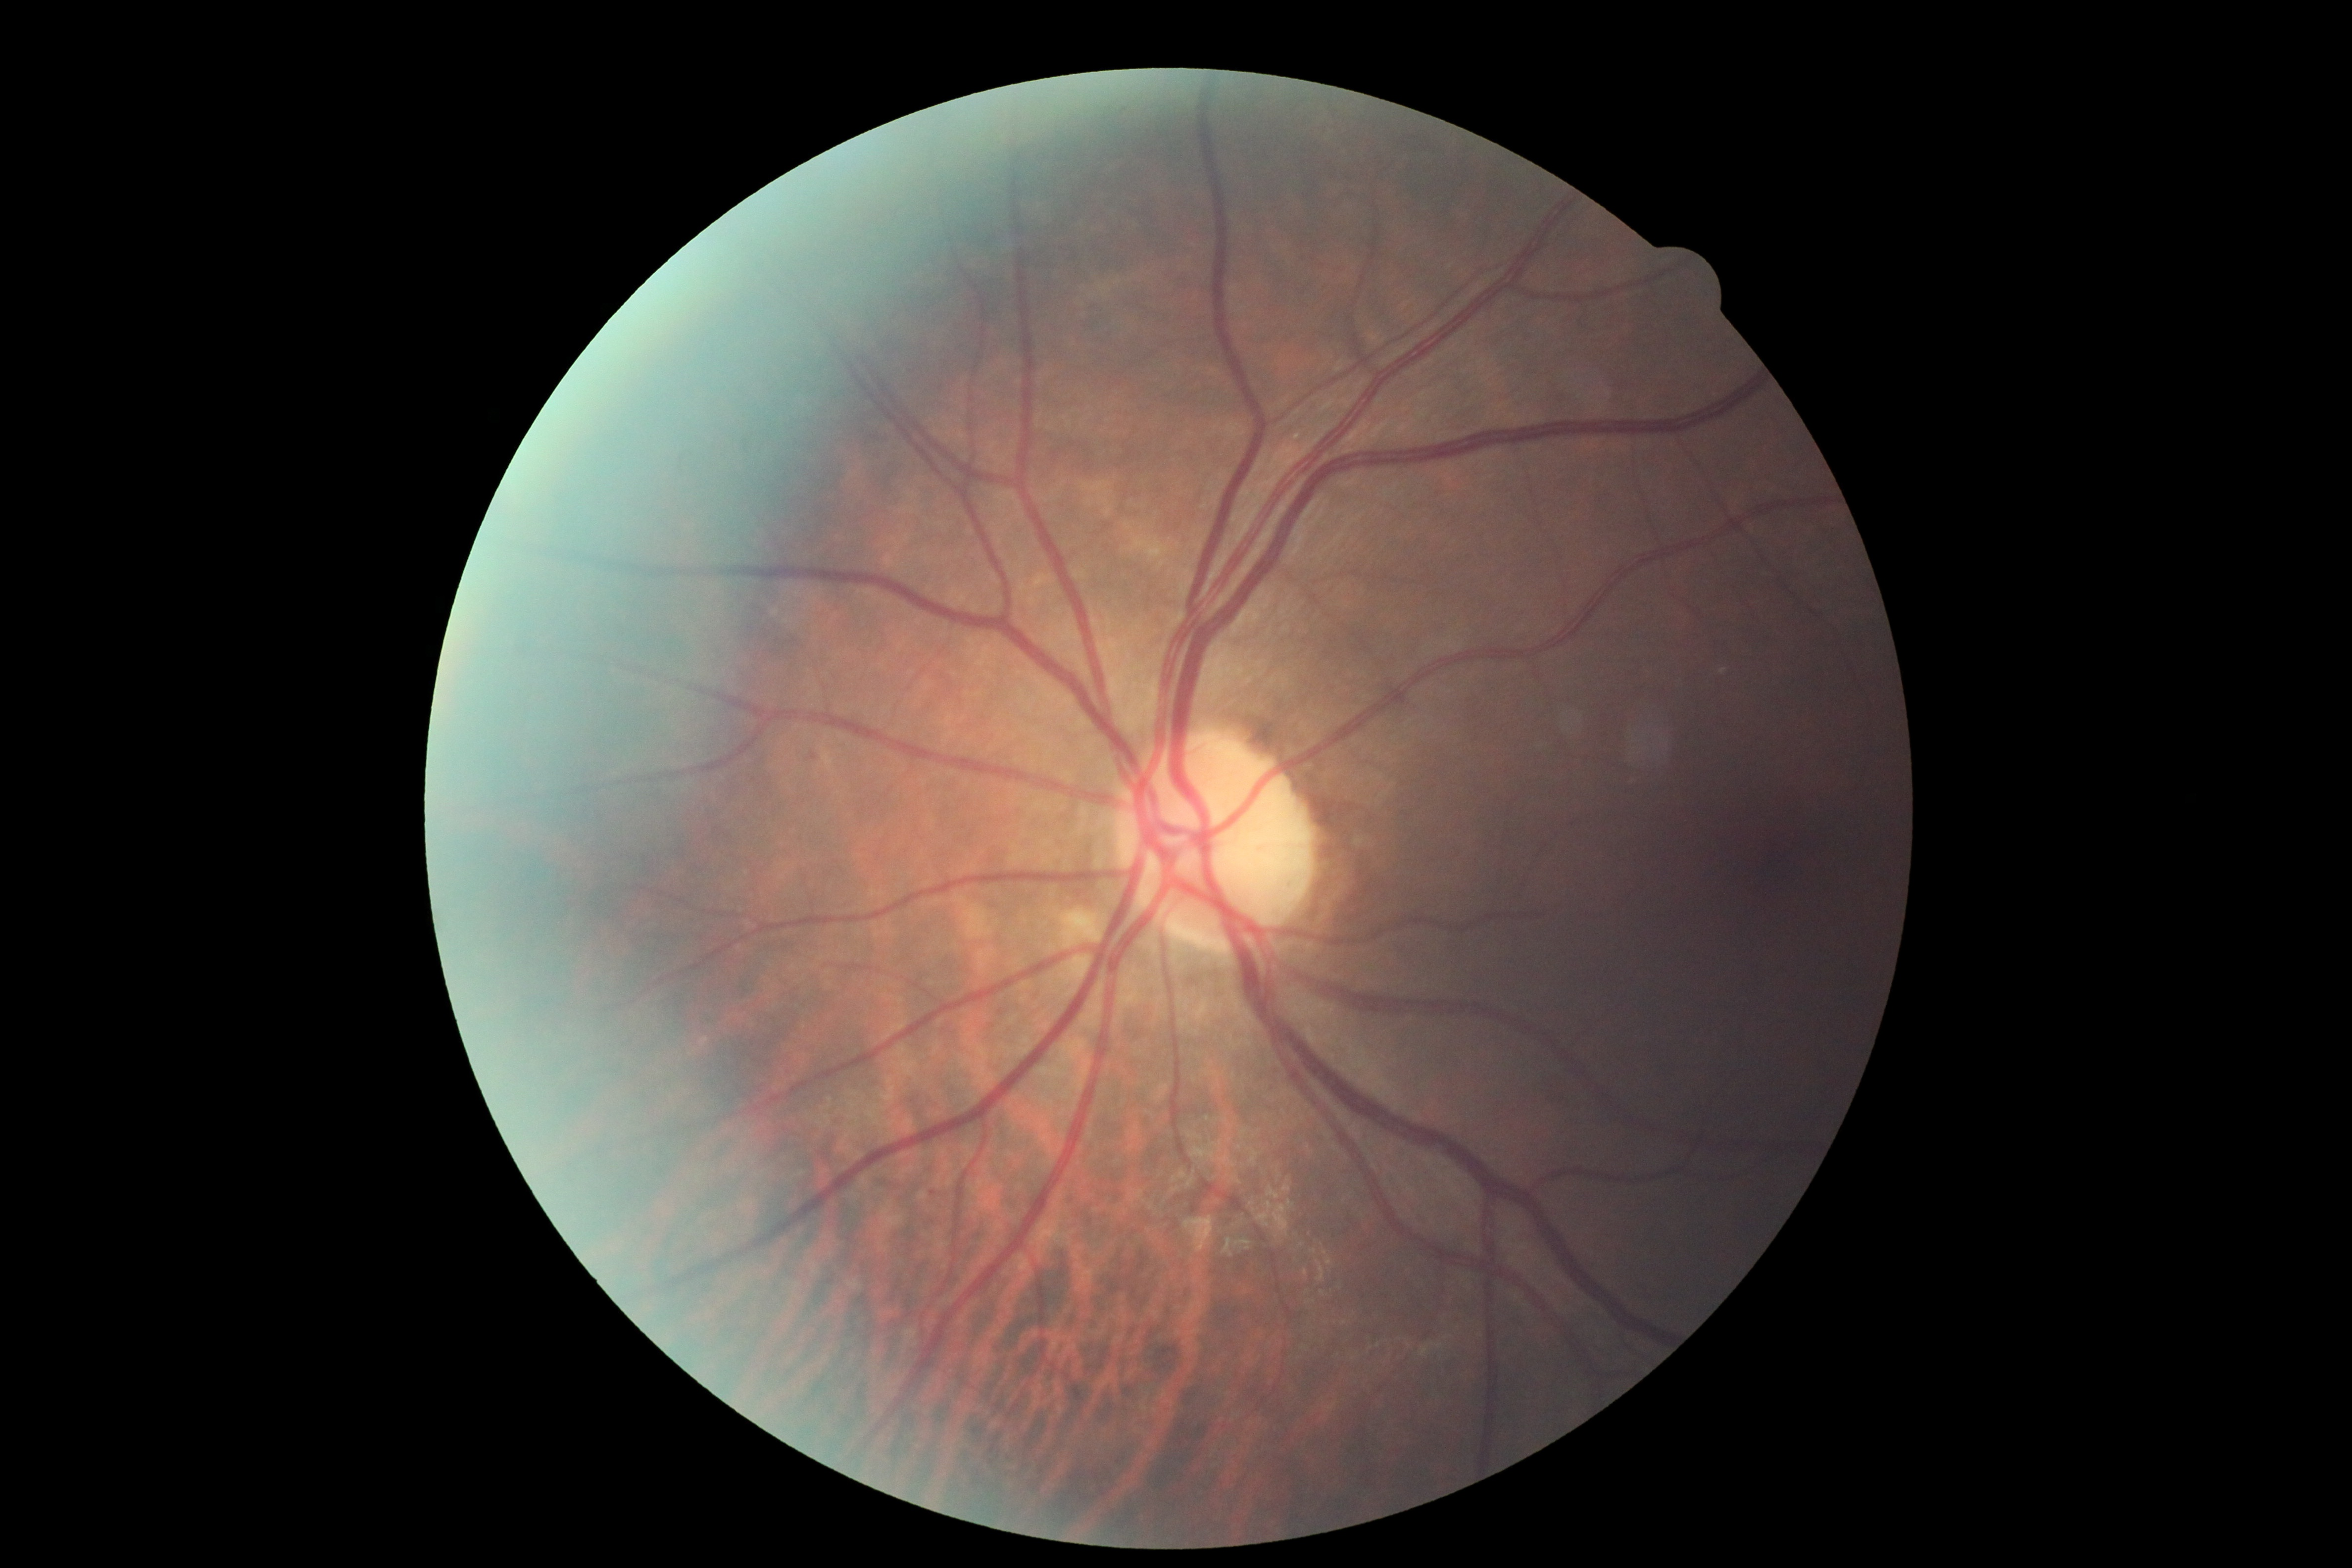
\includegraphics[width=0.8\linewidth]{1.jpeg}
  \caption{Ολόκληρος Αμφιβληστροειδής}
  \label{fig:2morfes1}
\end{subfigure}%
\begin{subfigure}{.5\textwidth}
  \centering
  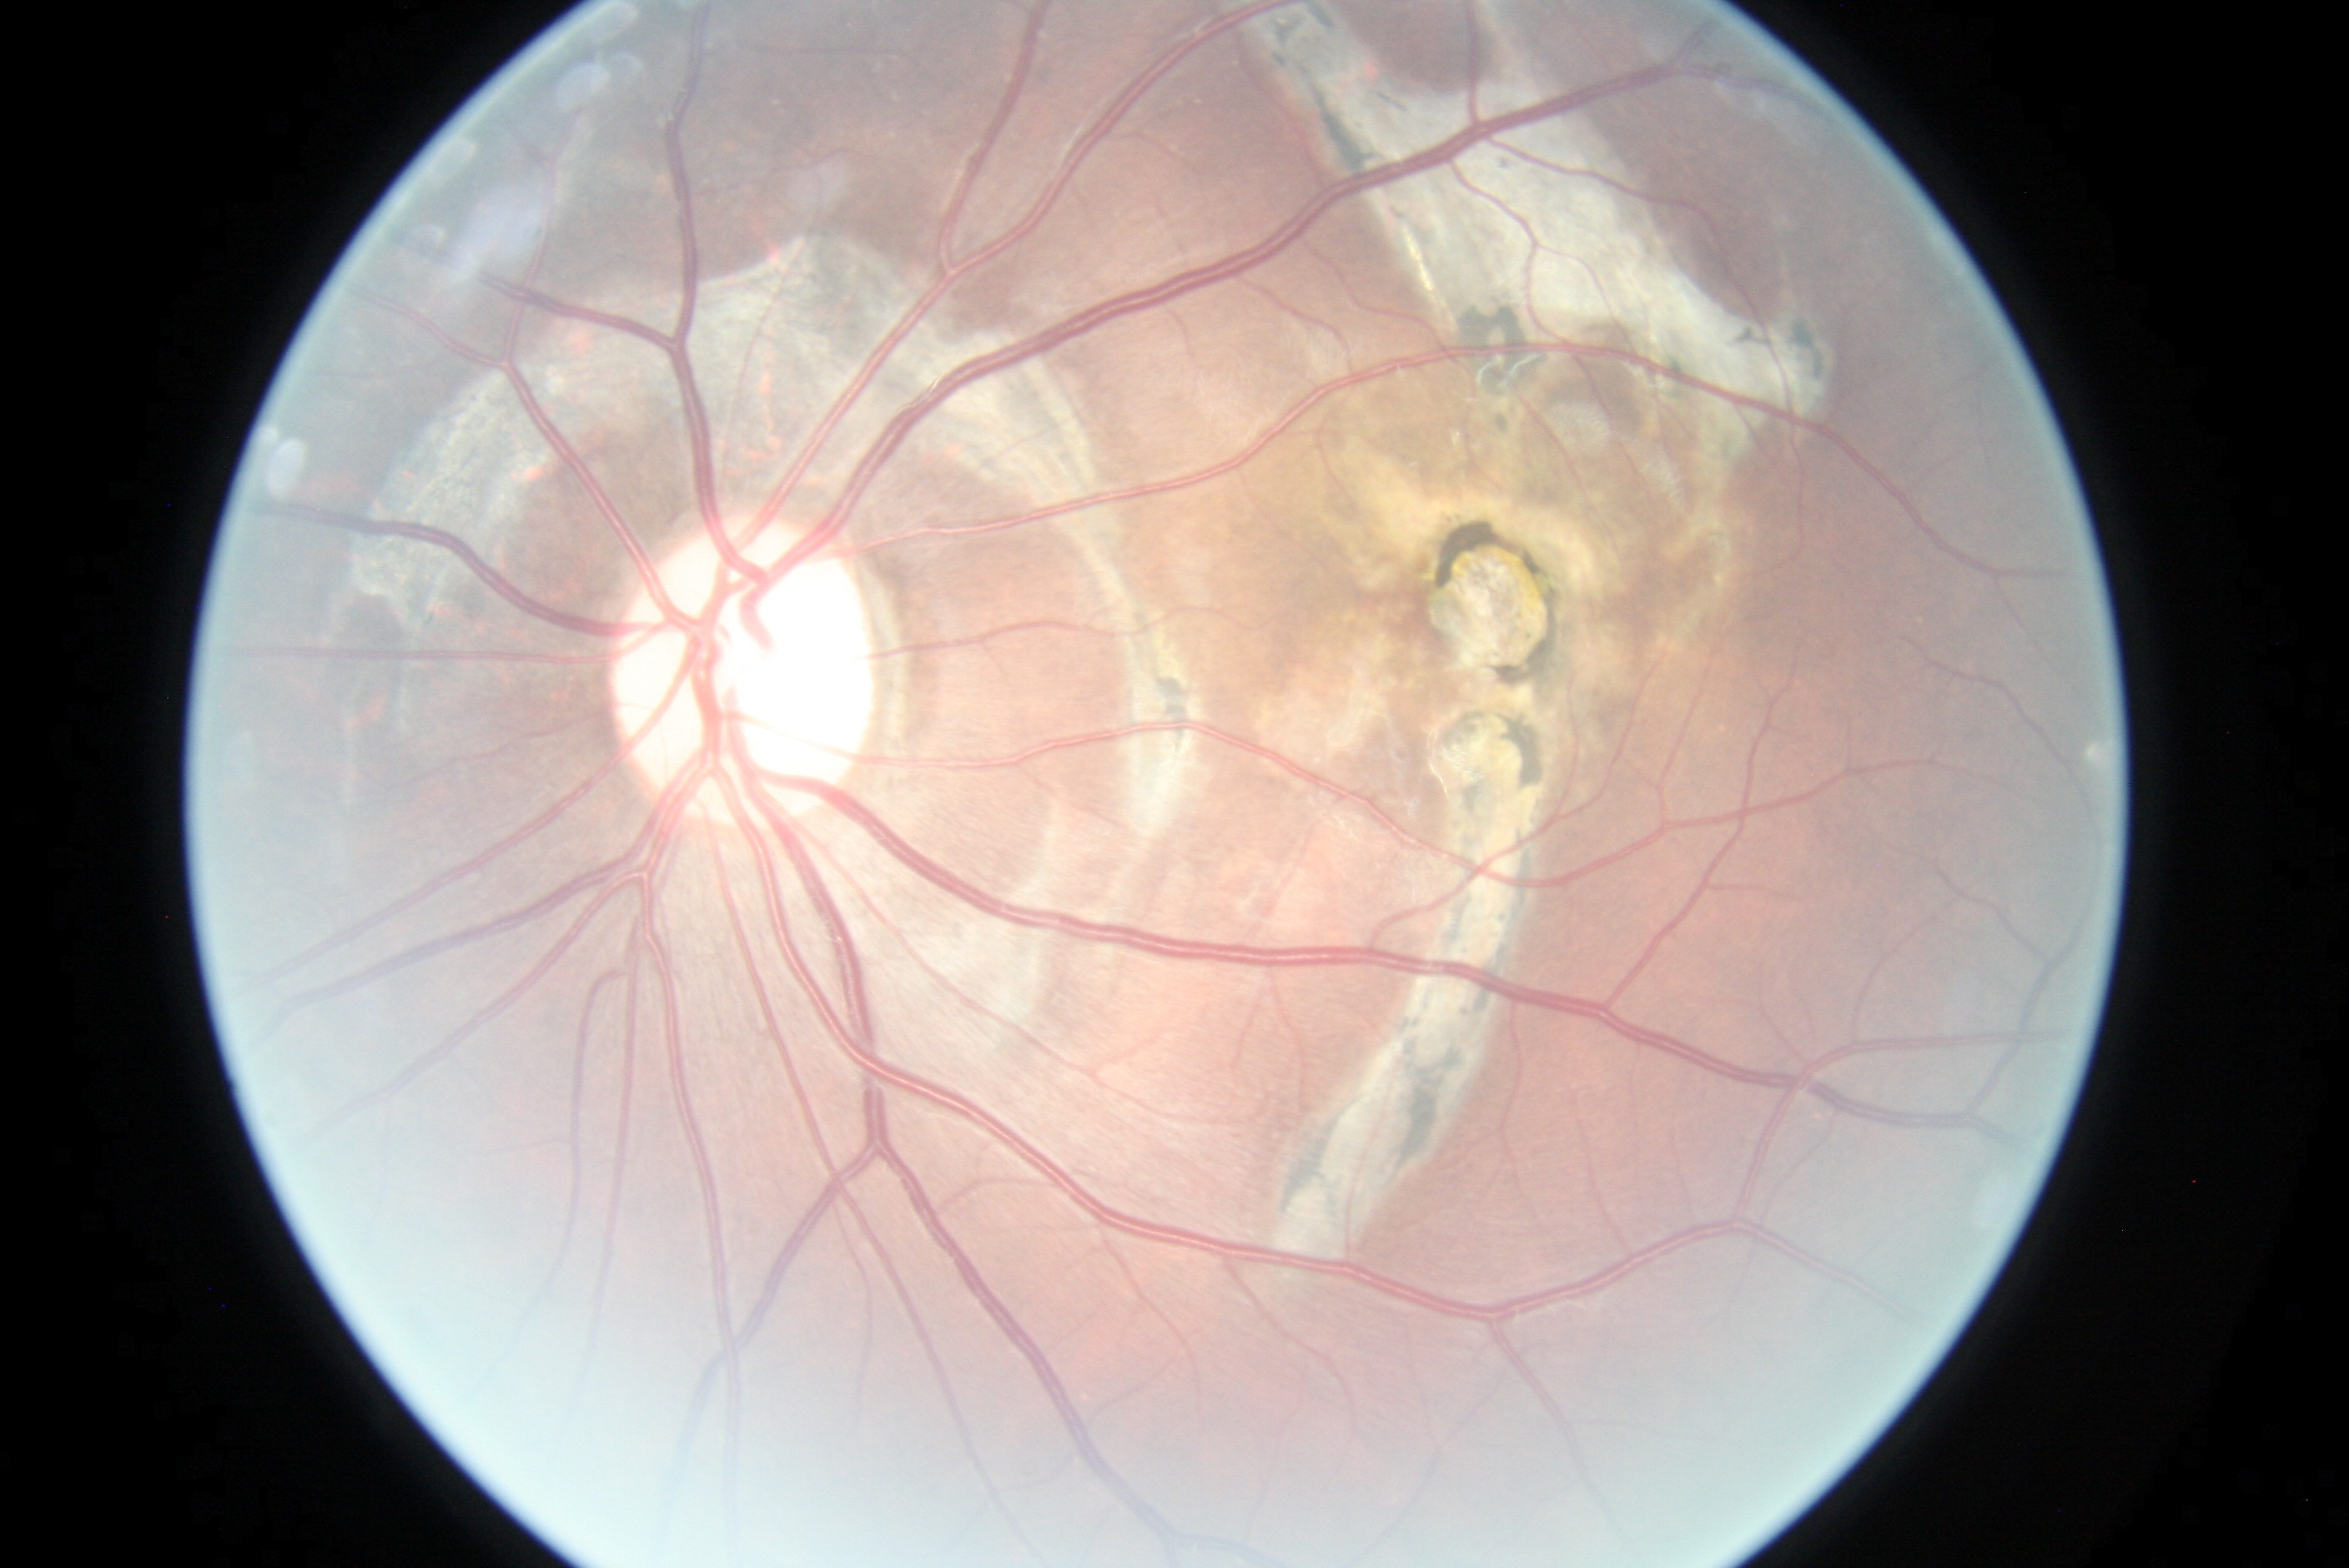
\includegraphics[width=0.8\linewidth]{2.jpeg}
  \caption{Κομμένος πάνω και κάτω Αμφιβληστροειδής}
  \label{fig:2morfes2}
\end{subfigure}
\caption{Δύο μορφές αμφιβληστροειδούς}
\label{figure:2morfes}
\end{figure}
  
Αφού βρεθεί το κέντρο και η ακτίνα του κύκλου με τον μετασχηματισμό Hough, κόβουμε την εικόνα με κέντρο το κέντρο του κύκλου, κρατώντας ένα παράθυρο με διαστάσεις [2ακτίνα x 2ακτίνα]. Στην περίπτωση του μη ολόκληρου αμφιβληστροειδούς ακολουθείται η ίδια διαδικασία με την διαφορά ότι στο πάνω και κάτω μέρος προστίθενται όσα μηδενικά απαιτούνται για να καταλήξουμε στην [2ακτίνα x 2ακτίνα] εικόνα. Τέλος, μειώνεται το μέγεθος της εικόνας, στο μέγεθος που θα δοθεί ως είσοδο στο νευρωνικό, δηλαδή $299x299$. Στην \ref{figure:kag3} και \ref{figure:mes3} παρουσιάζονται οι κομμένες εικόνες των συνόλων δεδομένων Kaggle και Messidor 2, αντίστοιχα.

\begin{figure}[!h]
    \centering
      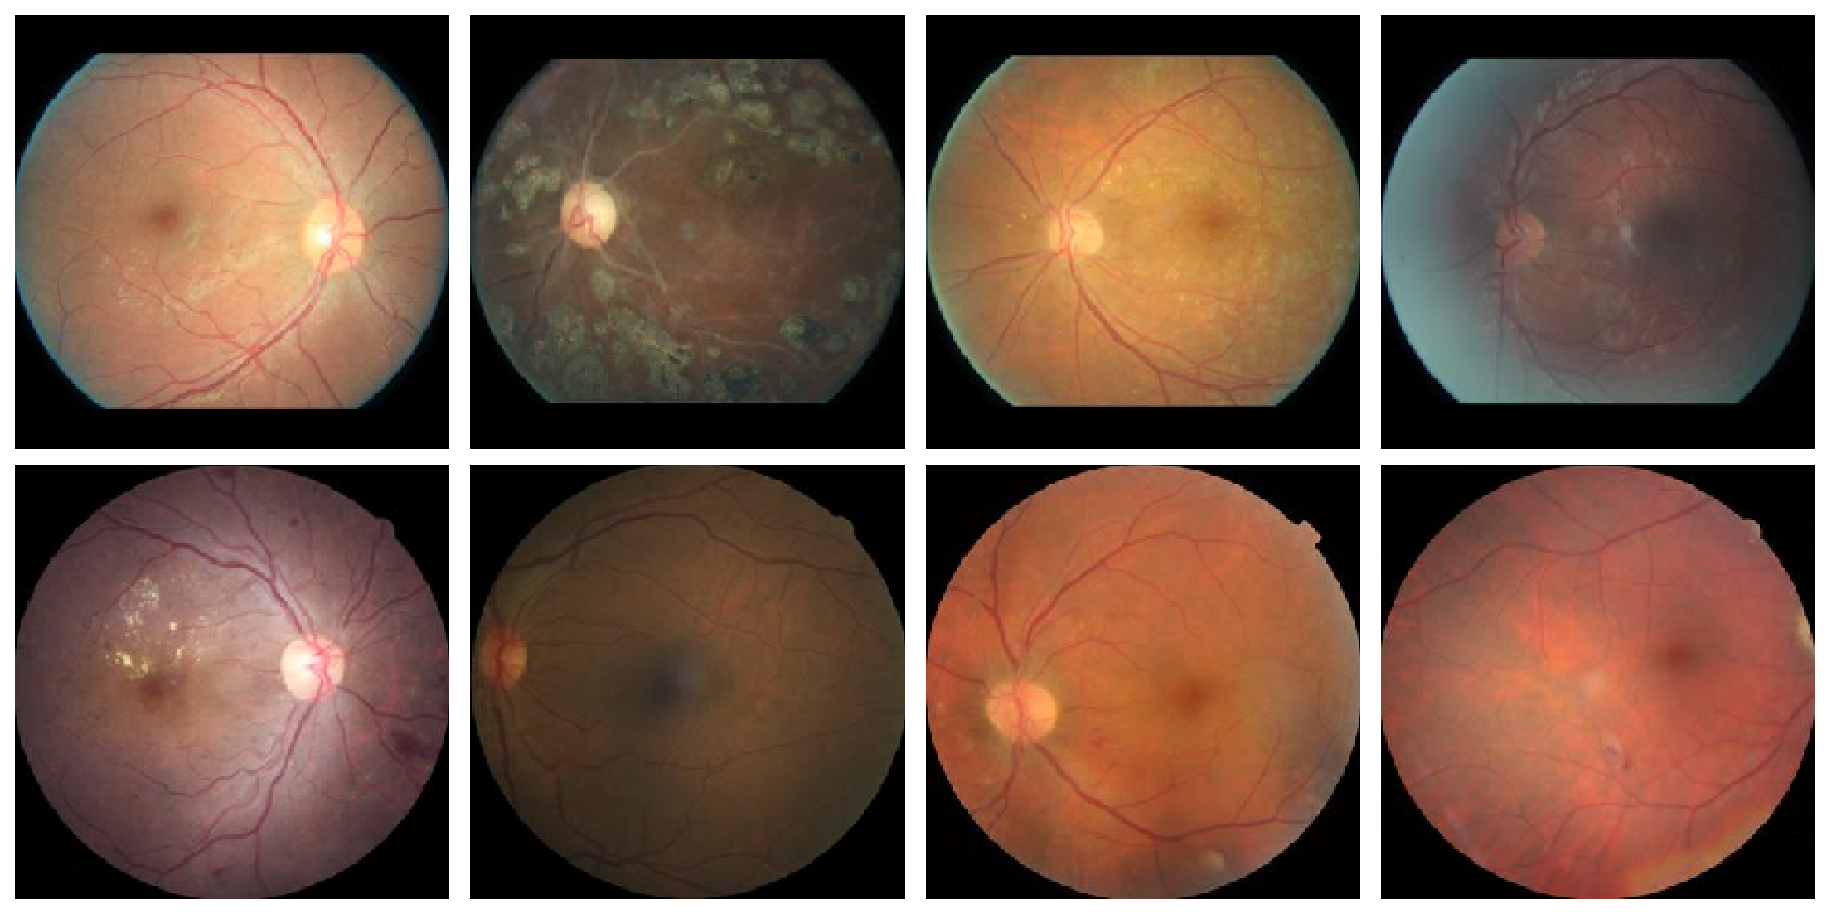
\includegraphics[width=1\linewidth]{kag3.pdf} \caption{Eνδεικτικά δείγματα κομμένων εικόνων του συνόλου δεδομένων Kaggle}
\label{figure:kag3}  
\end{figure}

\begin{figure}[!h]
    \centering
      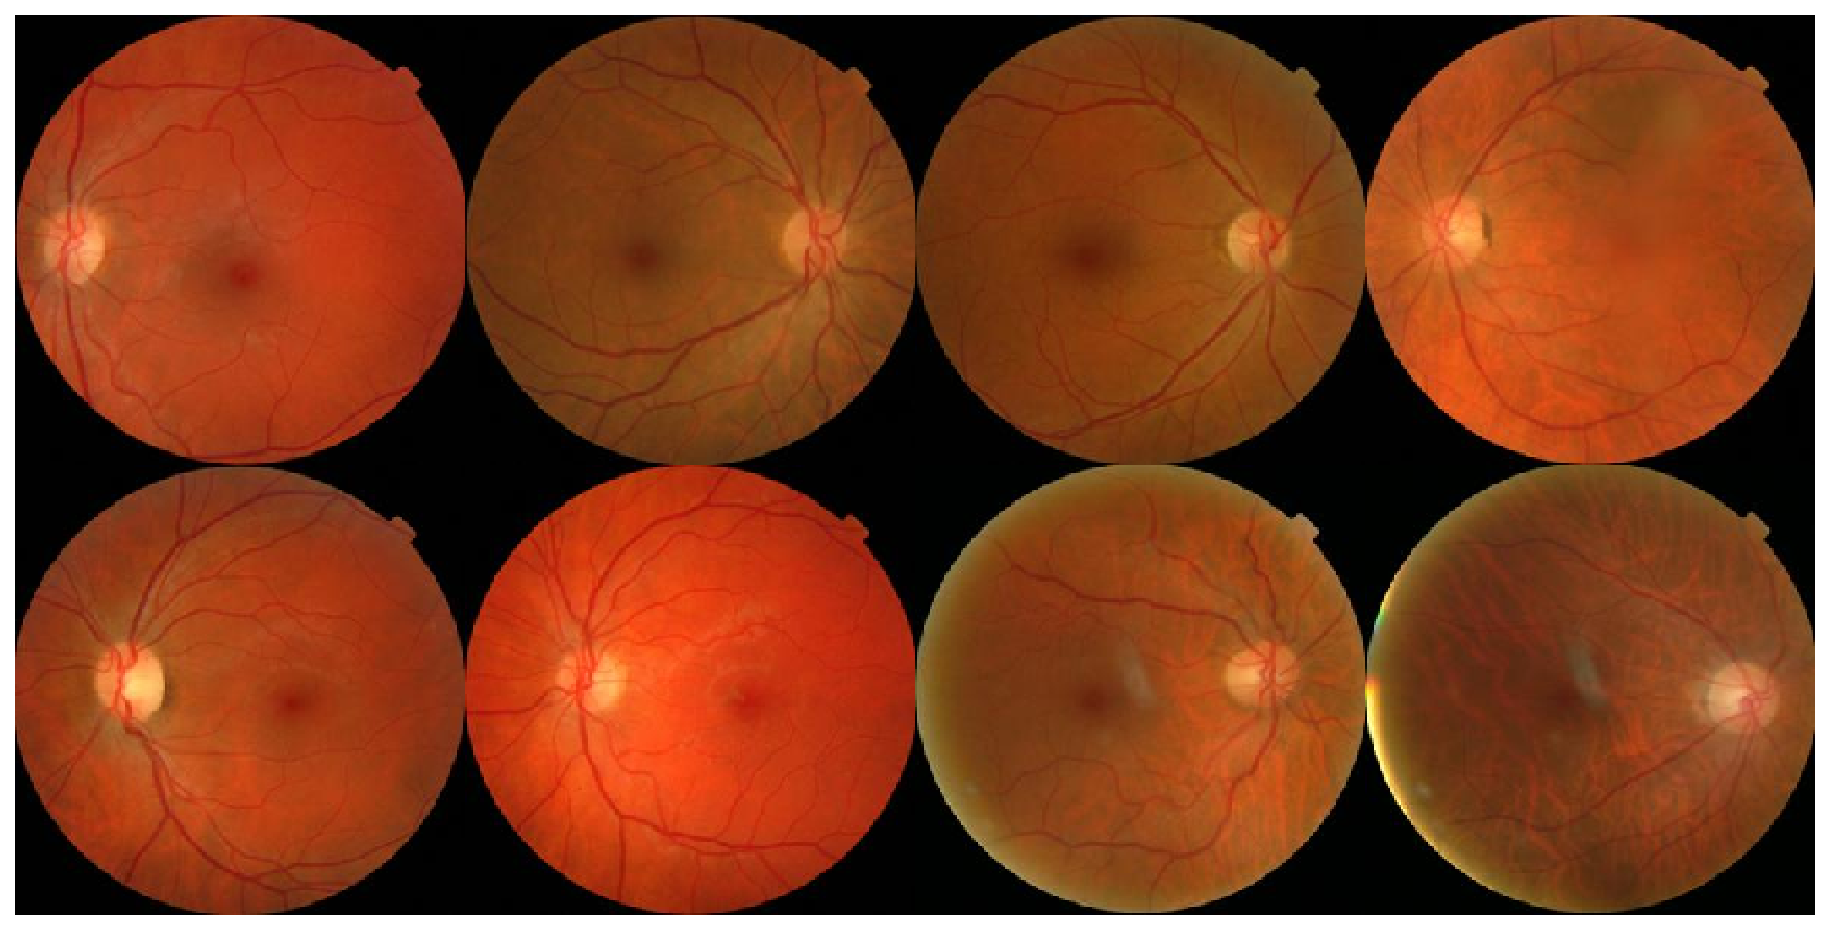
\includegraphics[width=1\linewidth]{mes.pdf} \caption{Eνδεικτικά δείγματα κομμένων εικόνων του συνόλου δεδομένων Messidor 2}
\label{figure:mes3}  
\end{figure}

\subsection{Μετασχηματισμός Hough} 
\label{sec:4.2.2}

Για την ανίχνευση του αμφιβληστροειδούς χρησιμοποιήθηκε ο μετασχηματισμός Hough\cite{Pedersen}. Ο μετασχηματισμός Hough μπορεί να περιγραφεί ως ένας μετασχηματισμός από το x,y επίπεδο, στο χώρο των παραμέτρων. Κάθε σχήμα απαιτεί διαφορετικό αριθμό παραμέτρων για να περιγραφεί, για αυτό ο μετασχηματισμός Hough χρησιμοποιείται συνήθως για απλά σχήματα των οποίων οι παράμετροι ανήκουν στο $R^2$ ή $R^3$. 
Ένα κύκλος μπορεί να περιγραφεί από την εξίσωση:
\begin{equation} \label{eq:circle}
r^2 =  (x - α)^2 + (y - β)^2
\end{equation}

Ο κύκλος έχει τρεις παραμέτρους, τις α, β και r που τα α, β αποτελούν το κέντρο του κύκλου στους άξονες x, y αντίστοιχα και r είναι η ακτίνα του κύκλου. Η παραμετρική εξίσωση του κύκλου είναι:

\begin{equation} \label{eq:par1}
x = α + r cos(\theta)
\end{equation}

\begin{equation} \label{eq:par2}
y = β + r cos(\theta)
\end{equation}

O χώρος των παραμέτρων ανήκει στο $R^3$. Κάθε σημείο του κύκλου στο xy επίπεδο, αντιστοιχίζεται στο χώρο των παραμέτρων σε κύκλους με κέντρο το συγκεκριμένο σημείο και ακτίνες σε ένα ορισμένο διάστημα. 


Εικονοστοιχεία με μεγάλη κλίση προδίδουν ύπαρξη ακμής οπότε είναι δυνατόν να ανήκουν σε κύκλο. Στην εικόνα\ref{figure:circle} παρουσιάζεται ο μετασχηματισμός Hough για τον μαύρο κύκλο. Κάθε διακεκομμένος κύκλος αποτελεί την αντιστοίχιση ενός σημείου του κύκλου από το x,y-επίπεδο, στο χώρο των παραμέτρων, για σταθερή ακτίνα. Να σημειωθεί ότι ενώ στην εικόνα επιλέγεται μία σταθερή ακτίνα για την καλύτερη γραφική αναπαράσταση, κάθε σημείο του κύκλου προβάλλεται σε k κύκλους με ίδιο κέντρο και ακτίνα που περιορίζεται σε ένα διάστημα.


\begin{figure}[!h]
    \centering
      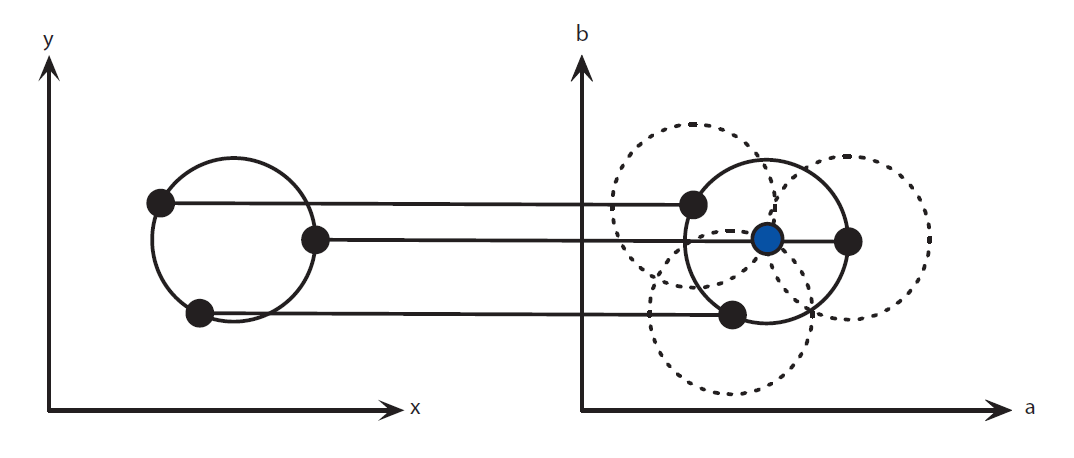
\includegraphics[width=0.5\linewidth]{hough2.PNG} \caption{Ο Μετασχηματισμός Hough από το x,y-επίπεδο(αριστερά), στο χώρο των παραμέτρων(δεξιά), για σταθερή ακτίνα}
\label{figure:circle}  
\end{figure}




Αν χωρίσουμε το χώρο σε ένα διακριτό πλέγμα, κάθε διακεκομμένος κύκλος ψηφίζει τα σημεία του. Όπως είναι φανερό το κέντρο του πραγματικού κύκλου θα βρίσκεται εκεί που θα υπάρχει μεγάλη συσσώρευση ψήφων καθώς οι διακεκομμένοι κύκλοι τέμνονται στο κέντρο του πραγματικού κύκλου.
Στην εικόνα \ref{figure:hough2} φαίνεται ο μετασχηματισμός Hough για μία εικόνα με 2 κύκλους. Ο μετασχηματισμός εφαρμόζεται για σταθερή ακτίνα r=20. Στο μετασχηματισμένο χώρο είναι φανερό ότι υπάρχει συσσώρευση ψήφων, στο κέντρο του πραγματικού κύκλου r=20. Καθώς το διάγραμμα είναι 2-d η συσσώρευση ψήφων αναπαριστάται με κόκκινο χρώμα. Επιπλέον, να σημειωθεί ότι το κέντρο του κύκλου με ακτίνα r = 25 δεν αναπαριστάται στο επίπεδο παραμέτρων, καθώς ο μετασχηματισμός Hough υπολογίστηκε για σταθερή ακτίνα r = 20.

\begin{figure}[!h]
\centering
\begin{subfigure}{.5\textwidth}
  \centering
  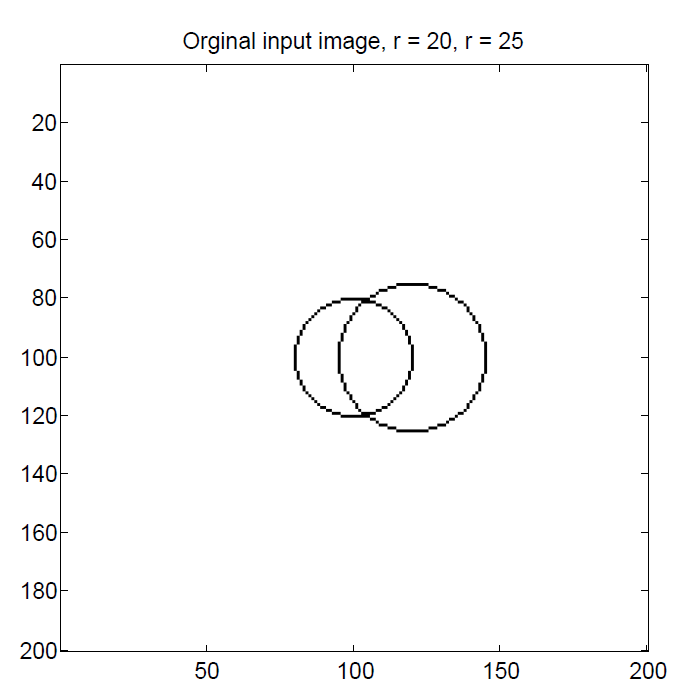
\includegraphics[scale=0.5]{h1.PNG}
  \caption{Εικόνα εισόδου}
  \label{fig:sub1bnew}
\end{subfigure}%
\begin{subfigure}{.4\textwidth}
  \centering
  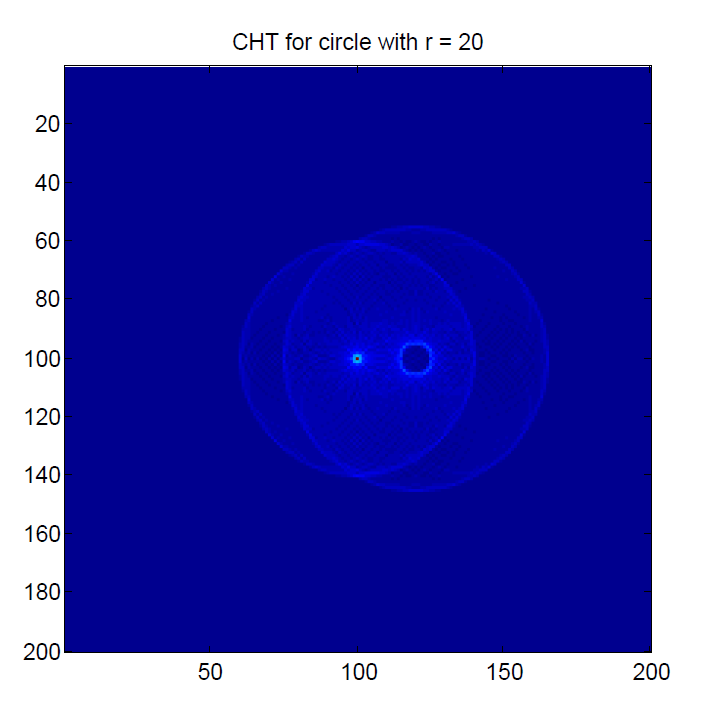
\includegraphics[scale=0.5]{h2.PNG}
  \caption{Μετασχηματισμός Hough για r = 20}
  \label{fig:sub2bnew}
\end{subfigure}
\caption{ Παράδειγμα συσσωρευτή του Μετασχηματισμού Hough για πραγματικά δεδομένα και σταθερή ακτίνα r = 20}
\label{figure:hough2}
\end{figure}



Για εύρεση κύκλου για μη σταθερή ακτίνα ακολουθείται η διαδικασία της ψηφοφορίας 
όπως περιγράφηκε για τη σταθερή ακτίνα με την προσθήκη ότι πια για κάθε κέντρο, υπάρχουν πολλοί κύκλοι λόγω της μη σταθερής ακτίνας. Οπότε πρέπει να επαναληφθεί ο αλγόριθμος της σταθερής ακτίνας για κάθε διαφορετική ακτίνα στο διάστημα που ορίστηκε. Αφού εφαρμοστεί, ο αλγόριθμος καταλήγει σε τριπλέτες $(α,β,r)$ για τους κύκλους που βρέθηκαν.



\chapter{Πειραματική Διαδικασία}
\label{chap:5}
\thispagestyle{plain}
Η εκπαίδευση του νευρωνικού έγινε σε μονάδα επεξεργασίας γραφικών NVIDIA GEFORCE RTX 2080 με 8GB μνήμη και έκδοση CUDA 10.1. Επιπλέον, έγινε χρήση Python version 2.7, Τensorflow version 1.13 και Κeras version 2.2.4.  

\section{CNN με εικόνες RGB}
\label{sec:5.1}

\subsection{Γενικά}
\label{subsec:5.1.1}
Για όλα τα πειράματα της παρούσας διπλωματικής έγινε χρήση του νευρωνικού Inception V3. 
Το νευρωνικό αυτό αρχικά χρησιμοποιήθηκε για την ανίχνευση 1000 κλάσεων από τη βάση δεδομένων του ImageNet οπότε στο  τελευταίο πλήρη συνδεδεμένο επίπεδο είχε 1000 νευρώνες. Για να προσαρμοστεί το νευρωνικό στο παρόν πρόβλημα, δηλαδή δυαδική ταξινόμηση ακολουθήθηκε η εξής διαδικασία: Κρατήθηκε η δομή του νευρωνικού μέχρι και το τελευταίο συνελικτικό επίπεδο το οποίο περιέχει 2048 φίλτρα διαστάσεων 8x8. Στα 2048 φίλτρα εφαρμόστηκε καθολική υποδειγματοληψία. Η καθολική υποδειγματοληψια είναι υποδειγματοληψια με μέγεθος παραθύρου, όσο η διάσταση της εικόνας, το οποίο σημαίνει ότι για κάθε εικόνα  8x8 υπολογίζεται μία τιμή μόνο, ως ο μέσος όρος των τιμών της εικόνας. Ουσιαστικά με αυτόν τον τρόπο τα δεδομένα προετοιμάζονται για την τελική πρόβλεψη. Άρα μετά την εφαρμογή της καθολικής υποδειγματοληψίας, το επόμενο επίπεδο θα έχει 2048 νευρώνες.  Τέλος, προστίθεται το τελευταίο επίπεδο με ένα νευρώνα μόνο, το οποίο αποτελεί το επίπεδο εξόδου για την τελική πρόβλεψη. 
 

Επιλέχθηκε η αρχικοποίηση των βαρών του μοντέλου με τα έτοιμα βάρη από την εκπαίδευση του δικτύου στις 1000 κλάσεις του Imagenet. Η χρήση έτοιμων βαρών προτιμήθηκε για γρηγορότερη σύγκλιση. Το μοντέλο με τα έτοιμα βάρη συγκλίνει γρηγορότερα λόγω της λειτουργίας των συνελικτικών δικτύων. Όπως αναφέρθηκε και παραπάνω, στα πρώτα επίπεδα το νευρωνικό μαθαίνει απλά σχήματα και δομές, στη συνέχεια οι δομές αυτές γίνονται πιο εξειδικευμένες ανάλογα με τις εικόνες εισόδου. Ουσιαστικά, μέσω της αρχικοποίησης με έτοιμα βάρη δίνουμε στο νευρωνικό έτοιμες τις απλές δομές αλλά συγχρόνως και τη δυνατότητα να τα αναπροσαρμόσει. Κατά η διάρκεια της εκπαίδευσης οι εικόνες του ImageNet κανονικοποιήθηκαν στο [-1,1], η ίδια λογική ακολουθήθηκε και στο παρόν πείραμα.

Καθώς ο αριθμός των εικόνων των δυο κλάσεων ήταν μη ισορροπημένος, με τον αριθμό εικόνων της κλάσης no rDR να είναι περίπου 4  φορές μεγαλύτερος, έγινε χρήση της κλάσης βάρους του Keras. Με την κλάση βάρους του Keras δίνεται μεγαλύτερο βάρος στην κλάση με το μικρότερο αριθμό εικόνων. 
Έτσι, κατά την εκπαίδευση μια εικόνα της κλάσης rDR, θα έχει τετραπλάσια βαρύτητα στους υπολογισμούς σε σχέση με μια εικόνα της κλάσης no rDR.


Κατά τη διάρκεια της εκπαίδευσης έγινε χρήση ModelCheckpoint του Keras, το οποίο ελέγχει κάθε εποχή κάποια  επιλεγμένη μετρική και δίνει τη δυνατότητα αποθήκευσης του μοντέλου βάση των τιμών αυτής της μετρικής. Για την παρούσα διπλωματική επιλέχθηκε έλεγχος της μετρικής του σφάλματος επικύρωσης και αποθήκευση του μοντέλου με το μικρότερο σφάλμα επικύρωσης. Ως συνάρτηση σφάλματος χρησιμοποιήθηκε η Binary Cross-Entropy loss.

Το μοντέλο είχε 21.802.784 παραμέτρους, με τους 21.768.352 εκπαιδεύσιμους(Trainable) και 34.432 μην εκπαιδεύσιμους(Non-trainable). Μη εκπαιδεύσιμοι είναι οι παράμετροι που δεν θα ανανεωθούν ή δεν θα βελτισοποιηθούν κατά τη διάρκεια της εκπαιδευσης και θα πρέπει  καθοριστούν εκ των προτέρων ή να δοθούν ως είσοδοι. Παραδείγματα μη εκπαιδευσιμων παραμέτρων είναι ο αριθμός των κρυφών επιπέδων, τα μεγέθη τους και ο αριθμός των φίλτρων. 

Το μοντέλο εκπαιδεύτηκε για 40 εποχές, με μέγεθος πακέτου(batch size) 8 και ρυθμό εκμάθησης $0.5 \cdot 10^{-3}$ . Κάθε εποχή έπαιρνε περίπου 11 λεπτά και η συνολική διάρκεια εκπαίδευσης ήταν περίπου 7,5 ώρες. Στην εικόνα \ref{figure:cnnflow} δίνεται μία συνοπτική περιγραφή του πειράματος CNN με εικόνες RGB.



\begin{figure}[!h]
    \centering
      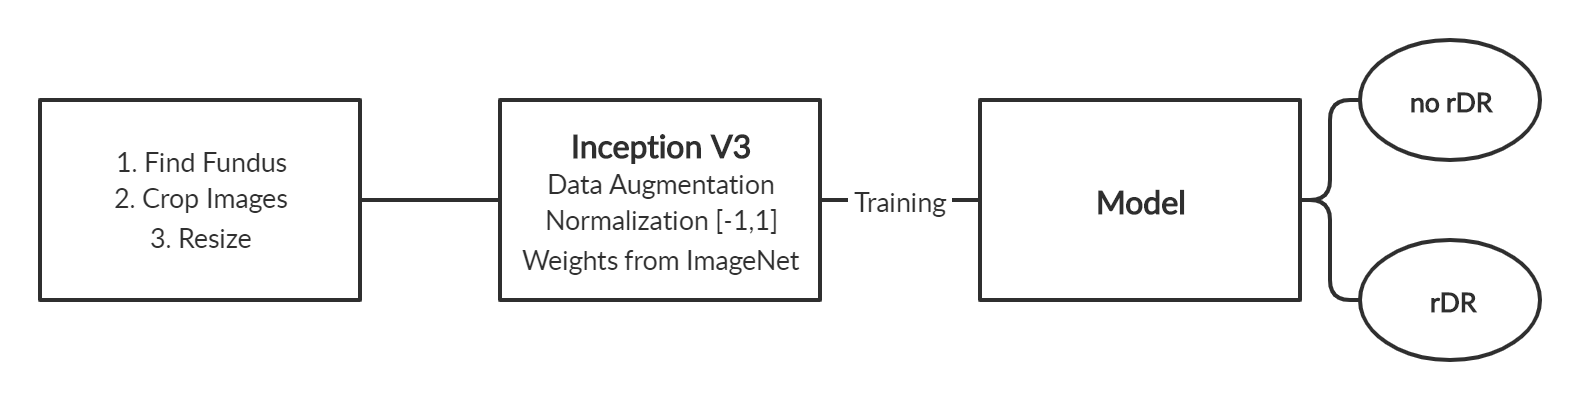
\includegraphics[width=1\linewidth]{cnn_flow.png} \caption{Συνοπτική περιγραφή του πειράματος CNN με εικόνες RGB}
\label{figure:cnnflow}  
\end{figure}



\subsection{Αύξηση Δεδομένων και Επεξεργασία Εικόνων}
\label{subsec:5.1.2}

Επίσης, έγινε αύξηση δεδομένων ώστε να επιτευχθεί καλύτερη ακρίβεια και μείωση της υπερεκπαιδευσης. Σε κάθε εποχή οι εικόνες μετασχηματίζονται με τυχαίο τρόπο ωστόσο ο  αριθμός των εικόνων παραμένει ίδιος. Άρα πρέπει να γίνει σαφές ότι οι εικόνες δεν αυξάνονται αλλά σε κάθε εποχή κάθε εικόνα υφίσταται ένα σύνολο μετασχηματισμών. Αύξηση δεδομένων αποτελείται μόνο στο σύνολο εκπαίδευσης και όχι στα σύνολο επικύρωσης και ελέγχου.

\subsubsection{Περιστροφή}
\label{subsubsec:5.1.2.1}


Επιλέχθηκε η χρήση αύξησης δεδομένων με περιστροφή ως προς το κέντρο της εικόνας κατά τυχαία γωνία στο διάστημα [0$^\circ$,360$^\circ$]. Σε πρώτη θεώρηση οι περιεστρεμμένες εικόνες φαίνονται μη ρεαλιστικές, καθώς η τυπική δομή περιέχει οπτικό δίσκο και ωχρά κηλίδα σε κάποιες σχετικά αναμενόμενες θέσεις  μέσα στην εικόνα. Για παράδειγμα μία ωχρά κηλίδα στο πάνω μέρος του αμφιβληστροειδούς θα ήταν μη ρεαλιστική. Ωστόσο, όπως αποδείχθηκε και με πειράματα με χρήση περιστροφής των εικόνων  δίνονται πολύ καλύτερα αποτελέσματα καθώς η ασθένεια είναι σταθερή σε σχέση με τη περιστροφή. Τέλος να σημειωθεί, ότι η αύξηση δεδομένων με περιστροφή έχει διττό ρόλο καθώς μειώνει το υπερεκπαίδευση και αυξάνει την ακρίβεια.



\subsubsection{Προσαρμογή Κορεσμού και Απόχρωσης}
\label{subsubsec:5.1.2.2}

Για την προσαρμογή του κορεσμού και της απόχρωσης μεταφέραμε την RGB εικόνα στο HSV χρωματικό χώρο\cite{HSV}. Ο χρωματικός χώρος HSV(απόχρωση, κορεσμός, φωτεινότητα) αποτελεί εναλλακτική αναπαράσταση του χρωματικού χώρου RGB και σχεδιάστηκε για να αναπαραστήσει καλύτερα  τον τρόπο με τον  οποίο οι άνθρωποι αντιλαμβάνονται το χρώμα. Η αναπαράσταση του HSV χρωματικού χώρου έχει κυλινδρική γεωμετρία όπως φαίνεται στην εικόνα \ref{figure:hsv}. Στον HSV χρωματικό χώρο τα χρώματα περιγράφονται μέσω του καναλιού της απόχρωσης(Hue). Η ποσότητα του γκρι σε ένα  χρώμα περιγράφεται μέσω του καναλιού του κορεσμού(Saturation) και η ένταση του χρώματος αναπαρίσταται με το κανάλι φωτεινότητας(Value).



\begin{figure}[!h]
    \centering
      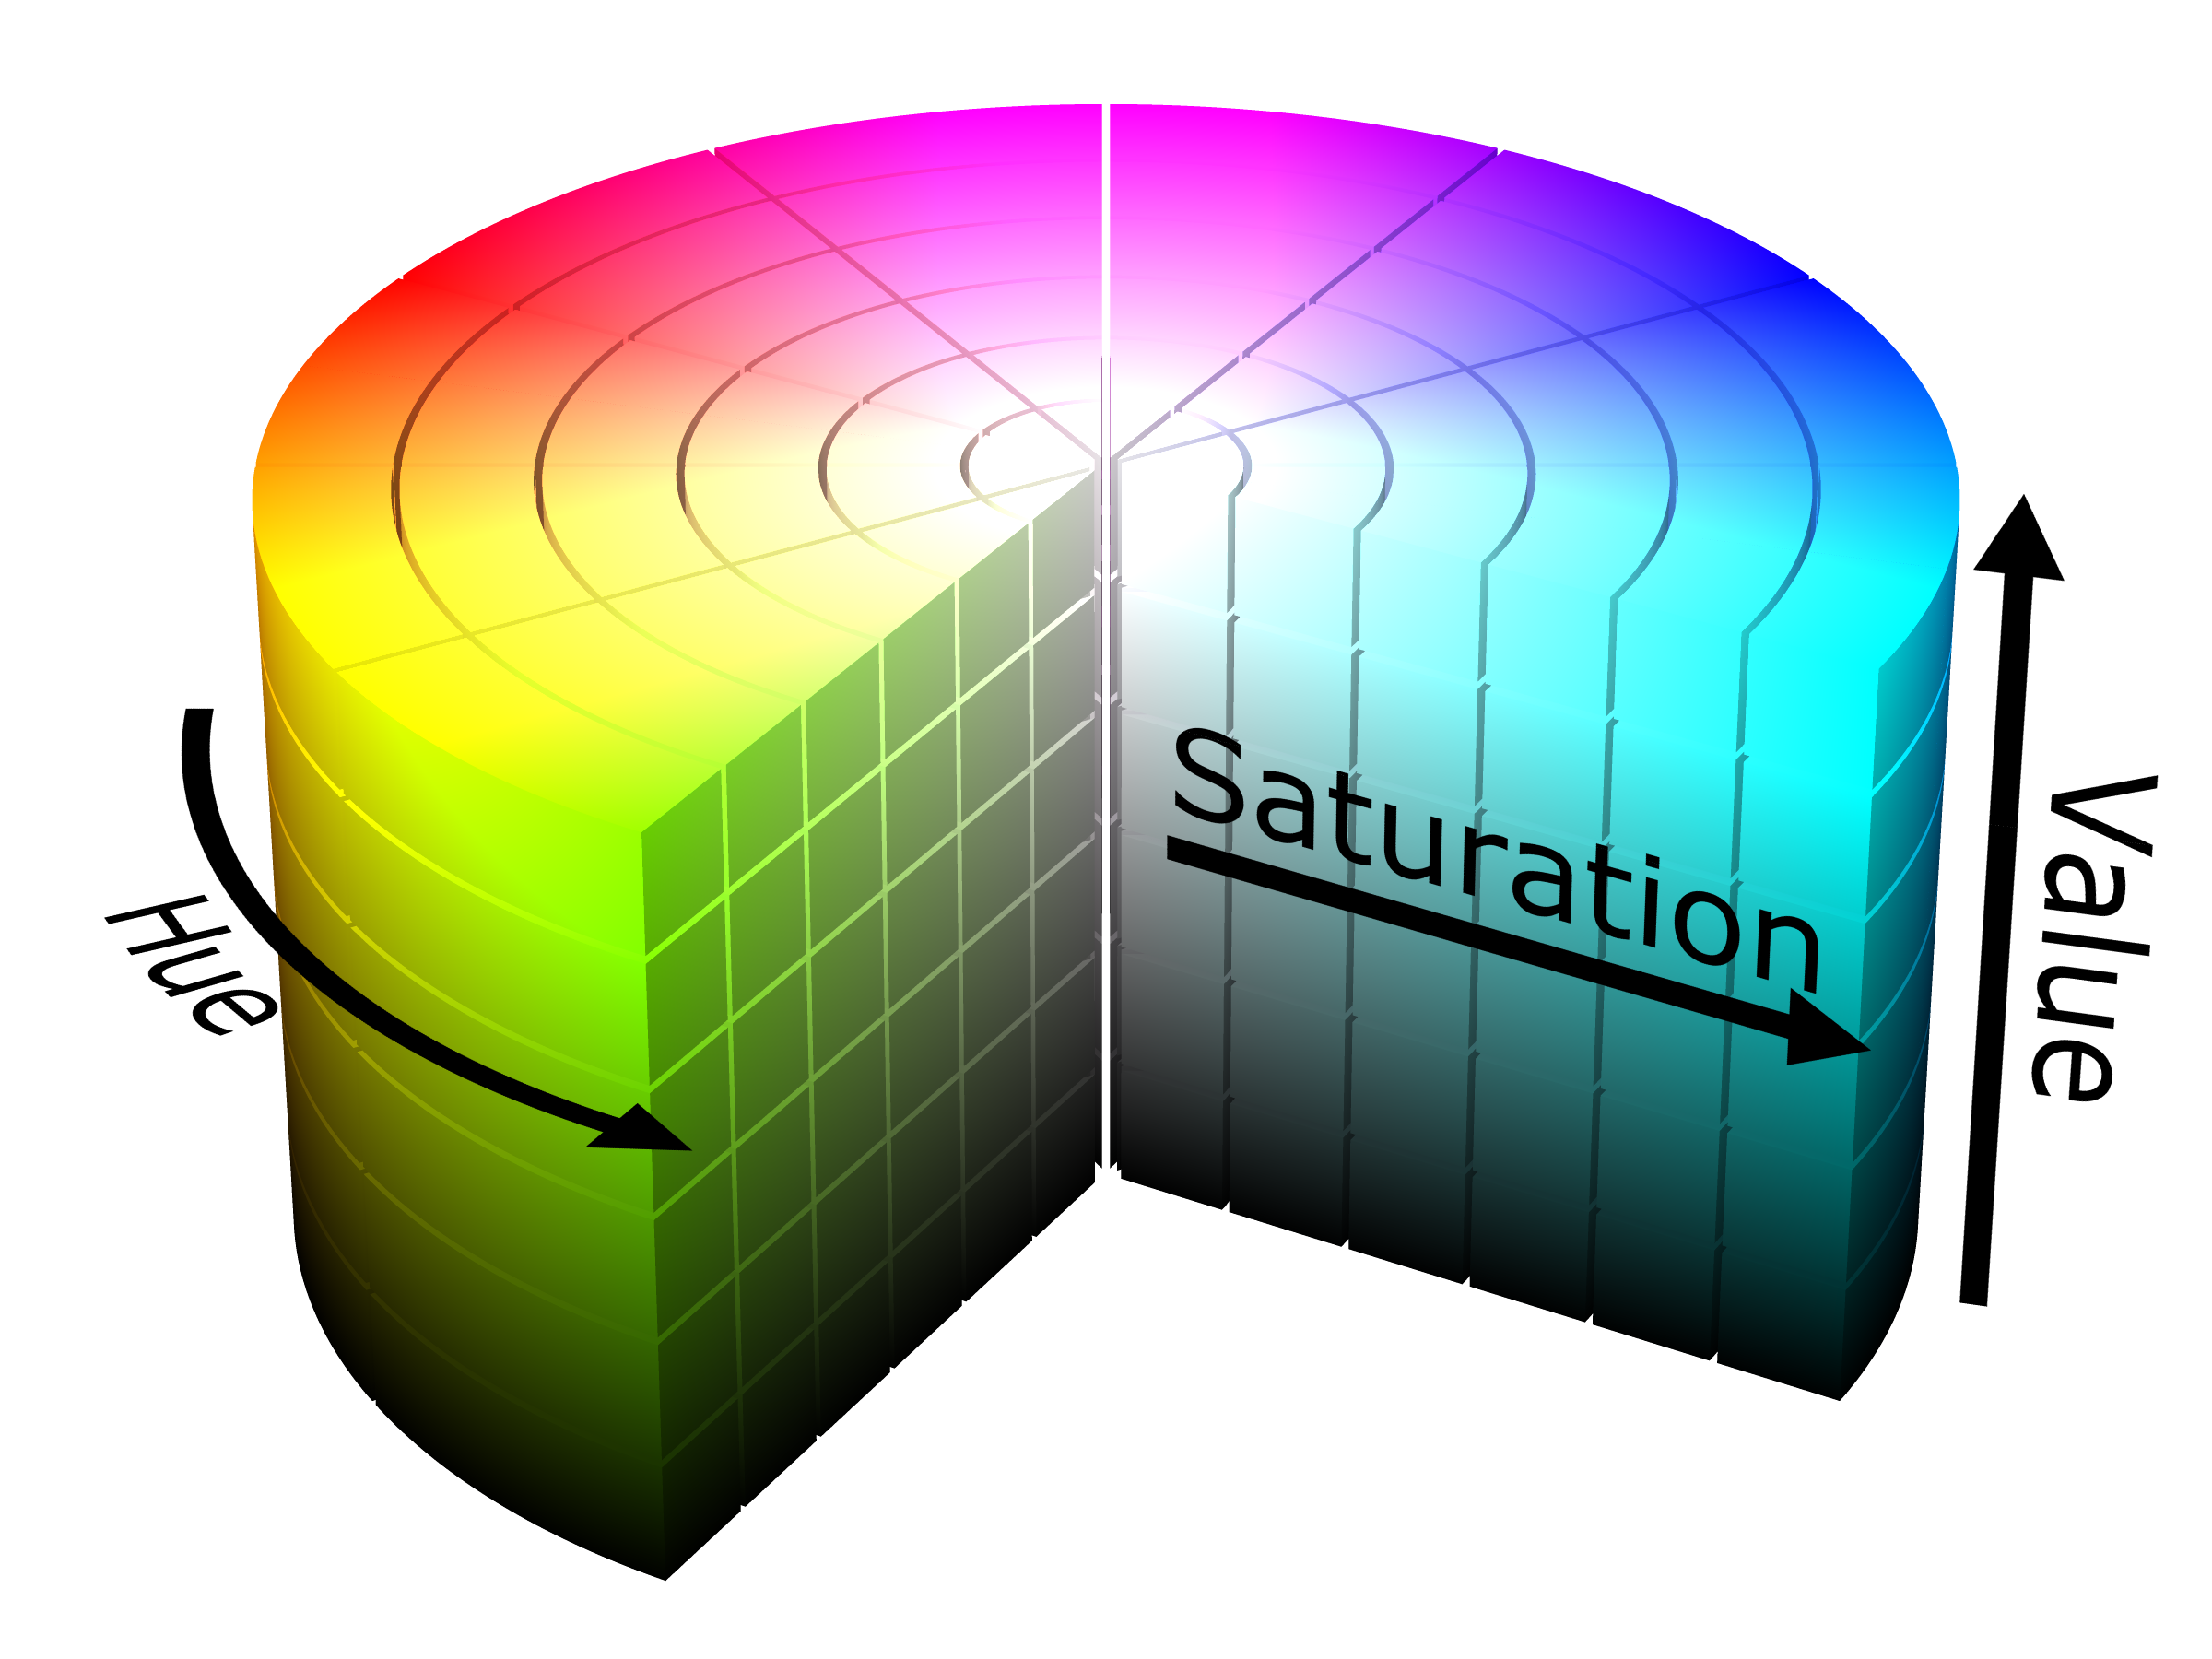
\includegraphics[width=0.6\linewidth]{hsv.png} \caption{Χρωματικός χώρος HSV}
      \label{figure:hsv}    
  \end{figure}


Το κανάλι της απόχρωσης αποτελεί τη γωνιακή συντεταγμένη. Ξεκινώντας από το κόκκινο στις 0$^\circ$ περνάει από το κίτρινο, το πράσινο, το γαλάζιο, το μπλε και το μωβ και καταλήγει μετά από πλήρη περιστροφή στο κόκκινο ξανά. Το κανάλι κορεσμού αποτελεί την ακτινική διάσταση και περιγράφει την ποσότητα γκρι σε ένα συγκεκριμένο χρώμα. Όσο πιο κοντά στο 0, τόσο πιο μεγάλη ποσότητα γκρι περιέχεται στο χρώμα. Το κανάλι φωτεινότητας  αποτελεί τη διάσταση του ύψους και περιγράφει την ένταση του χρώματος στο κλίμακα [0-100], όπου το 0 αντιστοιχίζεται στο μαύρο ενώ στο 100 έχουμε την μεγαλύτερη ένταση του χρώματος. Παρακάτω θα περιγραφεί ο τρόπος προσαρμογής της απόχρωσης και του κορεσμού. Τα διαστήματα τιμών για το κάθε κανάλι καθορίζονται από τον τρόπο αναπαράστασης του HSV χρωματικού χώρου στη Python.

Για την προσαρμογή της απόχρωσης προστίθεται σε όλα τα εικονοστοιχεία της εικόνας ένας σταθερός όρος στο διάστημα [0-5]. Η απόχρωση παίρνει τιμές στο διάστημα [0,179] και η αναπαράσταση της είναι κυκλική. Για τα εικονοστοιχεια των οποίων η τιμή της απόχρωσης είναι μεγαλύτερη από 180, επιστρέφεται το υπόλοιπο της διαίρεσης με το 180.

Για την προσαρμογή του κορεσμού προστίθεται σε όλα τα εικονοστοιχεία της εικόνας ένας σταθερός όρος στο διάστημα [-25, 25]. Το κανάλι κορεσμού παίρνει τιμές στο διάστημα [0, 255] οπότε  οι αρνητικές τιμές εικονοστοιχείων ή οι τιμές που ξεπερνούν το 255, τίθενται στο 0 και 255 αντίστοιχα. Να σημειωθεί ότι το διάστημα των σταθερών όρων  για τη προσαρμογή και την αντίθεση βρέθηκε πειραματικά ώστε να παράγονται ρεαλιστικά αποτελέσματα, δηλαδή εικόνες που θα μπορούσαν να ανήκουν στο σύνολο δεδομένων. 

\subsubsection{Προσαρμογή Φωτεινότητας και Αντίθεσης}
\label{subsubsec:5.1.2.3}


Για την προσαρμογή της φωτεινότητας και της αντίθεσης χρησιμοποιήθηκε ο μετασχηματισμός $α \cdot  f(i, j) +β$ που σύμφωνα με την βιβλιογραφία αλλάζει ταυτόχρονα φωτεινότητα και αντίθεση. \cite{Szeliski} \cite{Changing}. Η συνάρτηση $f(i,j)$ αναπαριστά την τιμή του μετασχηματισμένου εικονοστοιχείου (i,j) και τα α και β αποτελούν τις παραμέτρους προσαρμογής αντιθεσης και φωτεινοτητας, αντίστοιχα. 

Η χρήση του παραπάνω  μετασχηματισμού μπορεί να γίνει πιο κατανοητή με τα παρακάτω ιστογράμματα. Στον οριζόντιο άξονα ενός ιστογράμματος τοποθετούνται τα επίπεδα χρώματος μιας εικόνας, πχ για 8 bit εικόνα υπάρχουν 256 επίπεδα. Στον κατακόρυφο άξονα τοποθετείται ο αριθμός των εικονοστοιχείων που βρίσκεται σε ένα συγκεκριμένο επίπεδο χρώματος. Αν προστεθεί μια σταθερή θετική τιμή β σε όλα τα εικονοστοιχεία μίας εικόνας, τότε τα εικονοστοιχεία με τιμές μεγαλύτερες του 255 θα αντιστοιχιστούν στο 255. Αν προστεθεί μια σταθερή αρνητική τιμή β τότε τα εικονοστοιχεία με τιμές μικρότερες του 0 θα αντιστοιχιστούν στο 0. Με αυτόν τον τρόπο, στην πρώτη περίπτωση θα αυξηθεί η φωτεινότητα καθώς πιο πολλά εικονοστοιχεια θα βρεθούν στο 255, ενώ στη δεύτερη περίπτωση θα μειωθεί η φωτεινότητα καθώς πιο πολλά εικονοστοιχεια θα βρεθούν στο 0. Η αναπαράσταση της πρώτης περίπτωσης παρουσιάζεται στην εικόνα \ref{figure:b}. Με γκρι είναι το αρχικό ιστόγραμμα της εικόνας και με μαύρο το καινούριο ιστόγραμμα μετά από προσθήκη σταθερής θετικής τιμής σε όλα τα εικονοστοιχεια της εικόνας.

\begin{figure}[!h]
    \centering
      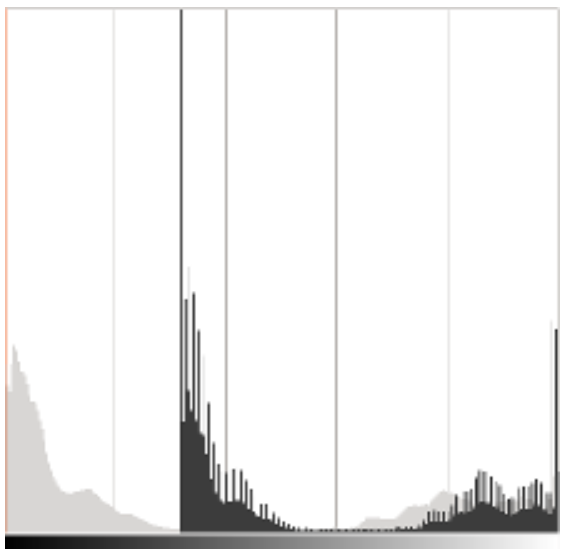
\includegraphics[width=0.4\linewidth]{b.PNG} \caption{Ιστόγραμμα εικόνας πριν(γκρι) και μετά(μαύρο) την πρόσθεση σταθερής τιμής b>0}
      \label{figure:b}    
  \end{figure}
  
Όσον αφορά την παράμετρο α, αυτή ρυθμίζει την έκταση  των τιμών στον οριζόντιο άξονα του ιστογράμματος. Για τιμές α<1, οι τιμές του οριζόντιου άξονα συμπιέζονται και η αντίθεση της εικόνας μειώνεται, καθώς περισσότερα εικονοστοιχεια αντιστοιχίζονται σε ίδιες τιμές του οριζόντιου άξονα. Αντίθετα για τιμές α>1 το ιστόγραμμα απλώνει και η εικόνα παρουσιάζει μεγαλύτερη αντίθεση. Η αναπαράσταση της παραπάνω περιγραφής παρουσιάζεται στην εικόνα \ref{figure:a}. Με γκρι είναι το αρχικό ιστόγραμμα της εικόνας ενώ με μαύρο το καινούριο ιστόγραμμα μετά από τον πολλαπλασιασμό με σταθερή θετική τιμή α<1 σε όλα τα εικονοστοιχεια της εικόνας.

\begin{figure}[!h]
    \centering
      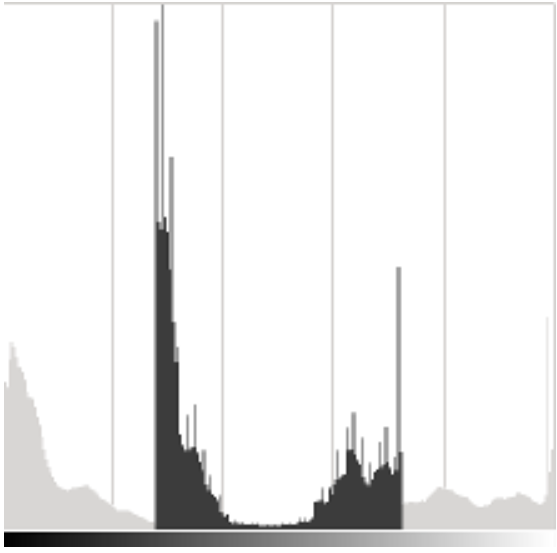
\includegraphics[width=0.4\linewidth]{a.PNG} \caption{Ιστόγραμμα εικόνας πριν(γκρι) και μετά(μαύρο) τον πολλαπλασιασμό με σταθερή τιμή α<1}
      \label{figure:a}    
  \end{figure}


Για την παρούσα διπλωματική, το εύρος τιμών για την παράμετρο προσαρμογής  αντίθεσης ορίστηκε στο διάστημα [0.5, 1.5] και για την παράμετρο προσαρμογής φωτεινότητας στο διάστημα [-40,40]. Μετά τον μετασχηματισμό, οι  αρνητικές τιμές εικονοστοιχείων ή οι τιμές που ξεπερνούν τα 255, τέθηκαν 0 και 255, αντίστοιχα. Στη περίπτωση προσαρμογής φωτεινότητας και αντίθεσης το διάστημα των παραμέτρων προσαρμογής βρέθηκε πειραματικά με γνώμονα την παραγωγή ρεαλιστικών εικόνων, δηλαδή εικόνων που θα μπορούσαν να ανήκουν στο σύνολο δεδομένων. 

\subsubsection{Κανονικοποίηση εικόνων}
\label{subsubsec:5.1.2.4}

Λόγω της αρχικοποίησης με έτοιμα βάρη, οι εικόνες εισόδου πρέπει να κανονικοποιηθούν στο [-1, 1]. Στην \ref{eq:norm}  δίνεται η διαδικασία που ακολουθείται για την τελική κανονικοποίηση στο [-1, 1].  Τα εικονοστοιχεία των αρχικών εικόνων  παίρνουν τιμές στο διάστημα [0, 255]. Αρχικά κάθε εικονοστοιχείο της εικόνας διαιρείται με 255 έτσι ώστε η εικόνα να κανονικοποιηθεί στο [0,1]. Στη συνέχεια αφαιρείται από κάθε εικονοστοιχείο η τιμή 0.5, και η εικόνα παίρνει τιμές στο [-0.5, 0.5]. Τέλος τα εικονοστοιχεια πολλαπλασιάζονται με την τιμή 2, άρα η εικόνα καταλήγει στην επιθυμητή κανονικοποίηση στο [-1, 1].


\begin{equation}
\label{eq:norm}
\begin{split}
x /= 255\\
x -= 0.5\\
x *= 2
\end{split}
\end{equation}

όπου x η εικόνα εισόδου. Όλες οι παραπάνω πράξεις εφαρμόζονται σε κάθε εικονοστοιχείο της εικόνας.



\subsubsection{Συνάρτηση επεξεργασίας}
\label{subsubsec:5.1.2.5}

Το Keras, εκτός των έτοιμων συναρτήσεων για μετασχηματισμό των δεδομένων κατά τη διάρκεια της εκπαίδευσης,  επιτρέπει τη χρήση μιας συνάρτησης επεξεργασίας που θα καλείται για κάθε εικόνα κάθε εποχή και μπορεί να περιέχει οποιοδήποτε κώδικα. 
Η συνάρτηση επεξεργασίας είναι ένα από τα πιο σημαντικά χαρακτηριστικά που προσφέρει το Keras για αύξηση δεδομένων και συγχρόνως δίνει τη δυνατότητα πειραματισμό με διαφόρους μετασχηματισμούς (αλλαγή χρωματικού χώρου, εξισορρόπηση χρώματος) χωρίς να απαιτείται ο μετασχηματισμός των εικόνων και η αποθήκευση τους πριν την έναρξη της εκπαίδευσης. 
Στην συνάρτηση μετασχηματισμού αρχικά εφαρμόζεται η περιστροφή της εικόνας, η οποία εξηγήθηκε παραπάνω, στις μισές εικόνες σε κάθε εποχή με τυχαία επιλογή των εικόνων. Έπειτα εφαρμόζονται προσαρμογή Κορεσμού-Απόχρωσης και Φωτεινότητας-Αντίθεσης και σε αυτή την περίπτωση οι μετασχηματισμοί εφαρμόζονται στις μούσες εικόνες σε κάθε εποχή με τυχαία επιλογή των εικόνων επιπλέον οι μετασχηματισμοί Κορεσμού-Απόχρωσης και Φωτεινότητας-Αντίθεσης γίνονται με τυχαία σειρά. Στην εικόνα\ref{figure:viz2}  παρουσιάζονται κάποιες εικόνες που έχουν υποστεί τους παραπάνω μετασχηματισμούς. Τέλος, εφαρμόζεται η συνάρτηση κανονικοποίησης στο διάστημα [-1,1]. 

\begin{figure}[!h]
    \centering
      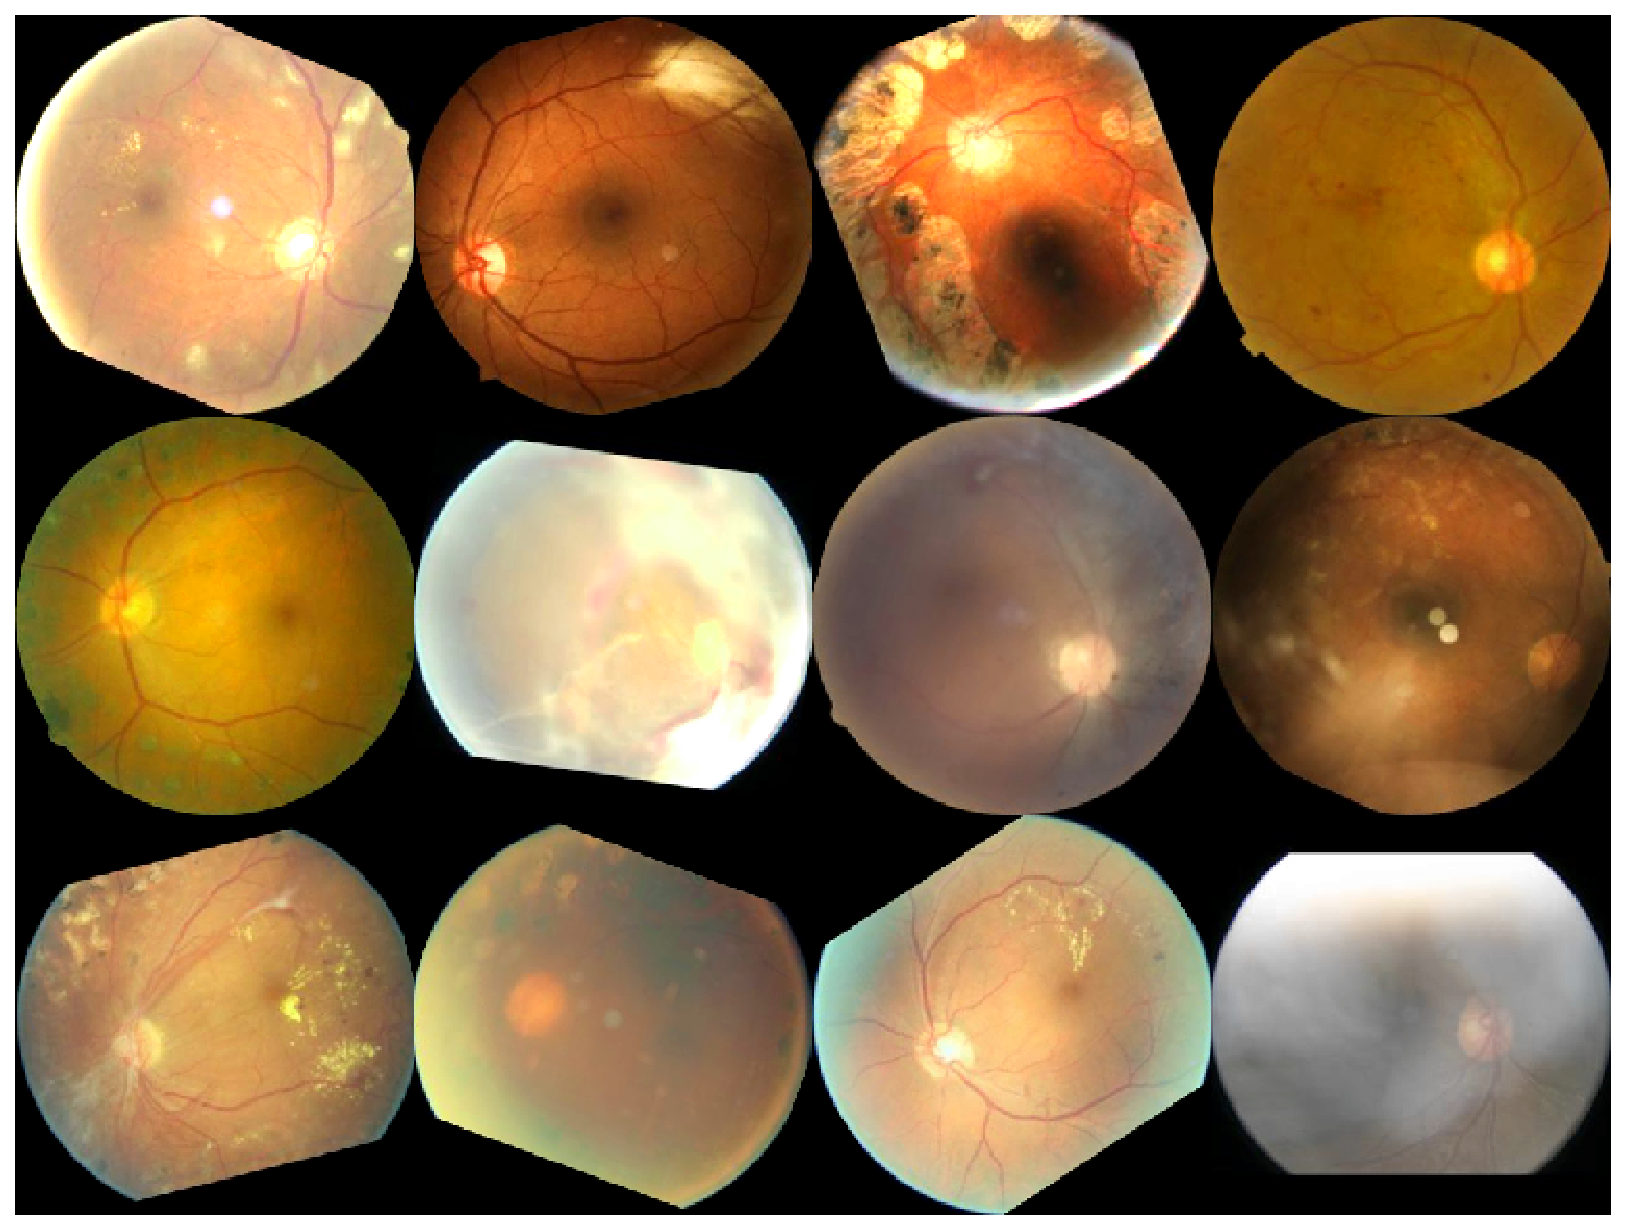
\includegraphics[width=1\linewidth]{vis2.pdf} \caption{Εικόνες που έχουν υποστεί περιστροφή και προσαρμογή φωτεινότητας, αντίθεσης, απόχρωσης και κορεσμού}
\label{figure:viz2}  
\end{figure}




\section{CNN με ταξινομητή SVM}
\label{sec:5.2}


Στο πείραμα με ταξινομητή Support Vector Machine ακολουθήθηκε η εξής διαδικασία. Μετά την εκπαίδευση  του νευρωνικού όπως εξηγήθηκε στην παραπάνω παράγραφο, δόθηκαν ως είσοδος στο μοντέλο τα σύνολα εκπαίδευσης και επικύρωσης και ανακτήθηκε ο χάρτης χαρακτηριστικών από το πρώτο πλήρη συνδεδεμένο επίπεδο με 2048 νευρώνες για κάθε εικόνα. Ο παραπάνω χάρτης χαρακτηριστικών είναι ένα διάνυσμα με 2048 νευρώνες και περιέχει την πληροφορία για τα χαρακτηριστικά που εντοπίστηκαν στην κάθε εικόνα. Έπειτα, το διάνυσμα με τις αντίστοιχες κλάσεις δόθηκε ως είσοδο στο μοντέλο SVM.
  Ουσιαστικά, αντί να δοθούν οι εικόνες στο ταξινομητή SVM, το οποίο μάλιστα θα ήταν αδύνατο λόγω του μεγάλου μεγέθους τους αλλά και της χωρικής πληροφορίας που περιέχουν και η οποία θα χάνονταν, δίνονται οι χάρτες χαρακτηριστικών με την αντίστοιχη κλάση που άνηκε η κάθε εικόνα από την οποία εξάχθηκαν. Επιπλέον, η πληροφορία των χαρτών χαρακτηριστικών είναι εξειδικευμένη στην ύπαρξη ή όχι rDR, καθώς τον νευρωνικό εκπαιδεύτηκε βάση αυτών των κλάσεων. Για την ταξινόμηση χρησιμοποιήθηκε ένας γραμμικός ταξινομητής SVM και ένας ταξινομητής με μη γραμμική συνάρτηση πυρήνα Radial basis. Στην εικόνα \ref{figure:cnnflowsvm} δίνεται μία συνοπτική περιγραφή του πειράματος CNN με ταξινομητή SVM.
  

  
\begin{figure}[!h]
    \centering
      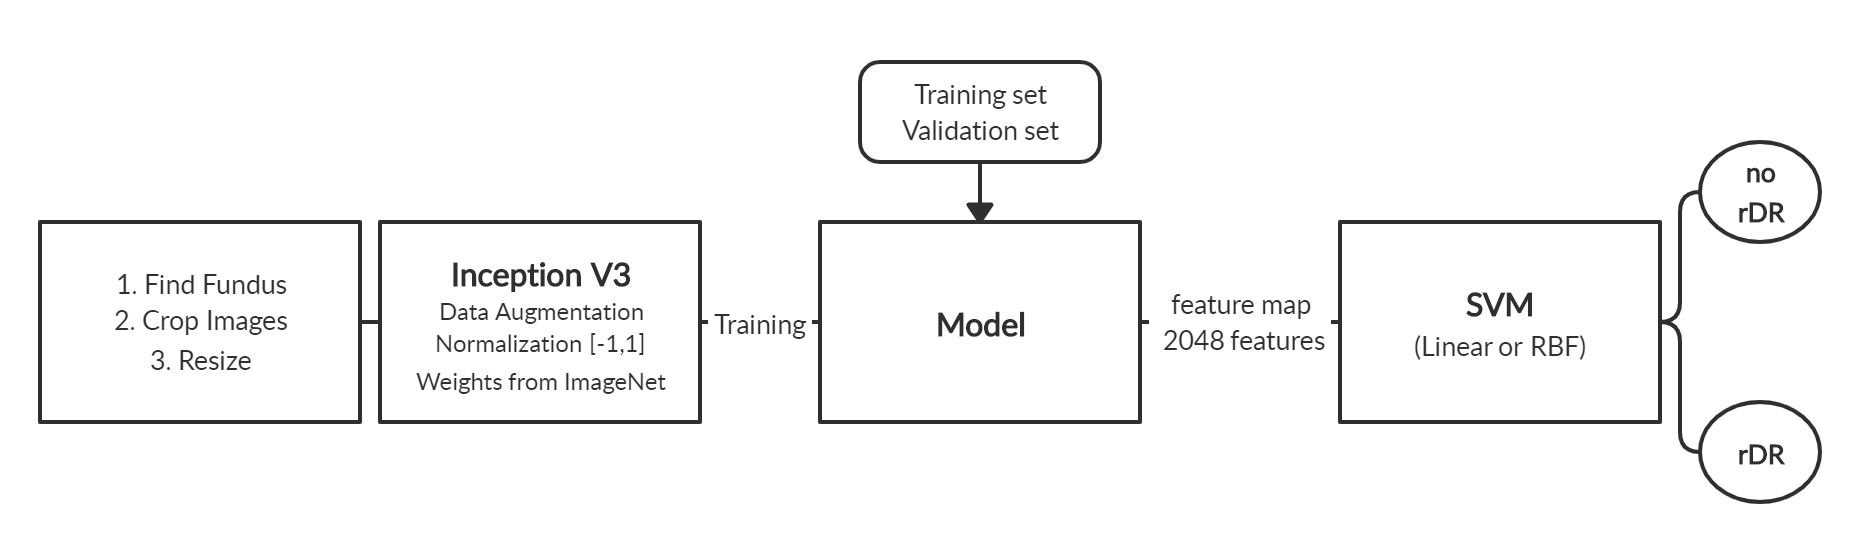
\includegraphics[width=1\linewidth]{cnn_svm_flow.png} \caption{Συνοπτική περιγραφή του πειράματος CNN με ταξινομητή SVM}
\label{figure:cnnflowsvm}  
\end{figure}


\section{Ensemble}
\label{sec:5.3}

Τα μοντέλα Ensemble συνδυάζουν τις αποφάσεις από πολλά μοντέλα για να βελτιώσουν την συνολική απόδοση. Επιπλέον βοηθούν στη βελτίωση της σταθερότητας και της ακρίβειας. Στην παρούσα διπλωματική εξετάστηκαν δύο μέθοδοι ensemble, το ensemble μέσης τιμής και ensemble με ψηφοφορία.
Για τις παραπάνω μεθόδους χρησιμοποιήθηκαν 9 μοντέλα. Τα 9 μοντέλο εκπαιδεύτηκαν για 40 εποχές, με μέγεθος πακέτου(batch size) 8 ή 32 εικόνες και διάφορους ρυθμούς εκμάθησης. Κάθε εποχή πήρε περίπου 11 λεπτά και η διάρκεια εκπαίδευσης ήταν περίπου 7,5 ώρες/μοντέλο. Να σημειωθεί ότι λόγω της αύξησης δεδομένων και των τυχαίων εικόνων που παράγονται κάθε φορά, μοντέλα που έτρεξαν με ίδιο μέγεθος πακέτου και ρυθμό εκμάθησης είναι δυνατόν να  παρουσιάσουν μικρές διαφορές ως προς το τελικο αποτέλεσμα. Αυτό είναι λογικό καθώς σε ένα πείραμα μπορεί να παραχθούν  εικόνες που θα κατευθύνουν καλύτερα το νευρωνικό στο να ανακαλύψει τα χαρακτηριστικά σχετικά με την ύπαρξη ή όχι της rDR.   
 
\subsection{Ensemble Μέσης Τιμής}
\label{subsec:5.3.1}
Στο ensemble μέσης τιμής αρχικά υπολογίζονται οι προβλέψεις (πιθανότητες) κάθε μοντέλου για το σύνολο ελέγχου. Έπειτα, για κάθε εικόνα αθροίζονται οι προβλέψεις από κάθε μοντέλο και διαιρούνται με τον αριθμό των μοντέλων. Η διαδικασία αυτή ακολουθείται για όλες τις εικόνες του συνόλου ελέγχου. Στο τέλος αυτής της διαδικασίας θα έχουν υπολογιστεί οι προβλέψεις του μοντέλου ensemble μέσης τιμής για το σύνολο ελέγχου. Όπως και στα απλά μοντέλα, για διάφορα κατώφλια υπολογίζεται η μετρική AUC και εξάγονται τα σημεία υψηλής ευαισθησίας και εξειδίκευσης, όπως επίσης και το βέλτιστο σημείο.  Στην εικόνα \ref{figure:avg} παρουσιάζεται η δομή του Ensemble μέσης τιμής.


\begin{figure}[!h]
    \centering
      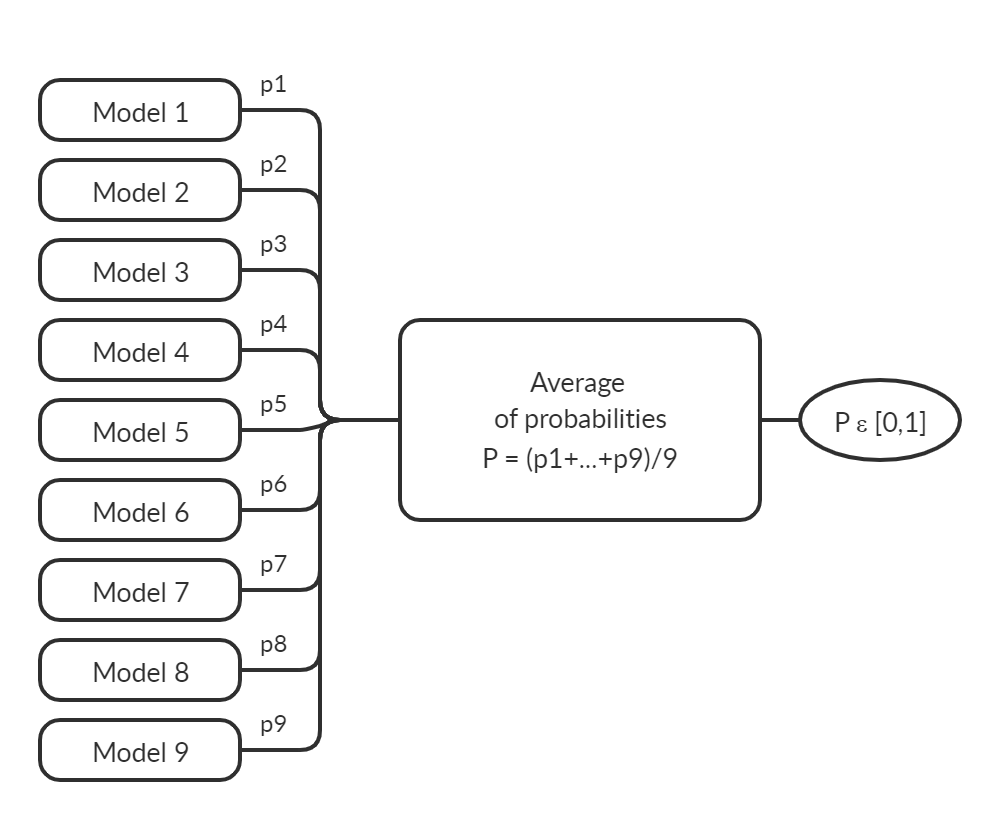
\includegraphics[width=0.6\linewidth]{avg.png} \caption{Ensemble μέσης τιμής για 9 μοντέλα}
      \label{figure:avg}    
  \end{figure}
 
\subsection{Ensemble με Ψηφοφορία}
\label{subsec:5.3.2}
Στο ensemble με ψηφοφορία αρχικά υπολογίζονται οι προβλέψεις κάθε μοντέλου για το σύνολο ελέγχου. 
Έπειτα για κάθε μοντέλο ακολουθείται η εξής διαδικασία: για διάφορα κατώφλια υπολογίζεται για κάθε εικόνα, η κλάση στην οποία ανήκει. Αφού υπολογιστούν τα παραπάνω. Για να υπολογιστεί η κλάση στην οποία ανήκει κάθε εικόνα για ένα συγκεκριμένα κατώφλι, το 9 μοντέλα ψηφίζουν. Αν για μία εικόνα πάνω από τα 4 μοντέλα έχουν ψηφίσει μια συγκεκριμένη κλάση, τότε αυτή είναι η νέα κλάση της εικόνας. Η παραπάνω διαδικασία θα επαναληφθεί για όλα τα κατώφλια. Στον τέλος βάση των κατωφλιών και των νέων κλάσεων των εικόνων, προκύπτει η μετρική AUC και τα σημεία υψηλής ευαισθησίας και εξειδίκευσης, όπως επίσης και το βέλτιστο σημείο. Στην εικόνα \ref{figure:voting} παρουσιάζεται η δομή του Ensemble με ψηφοφορία.

\begin{figure}[!h]
    \centering
      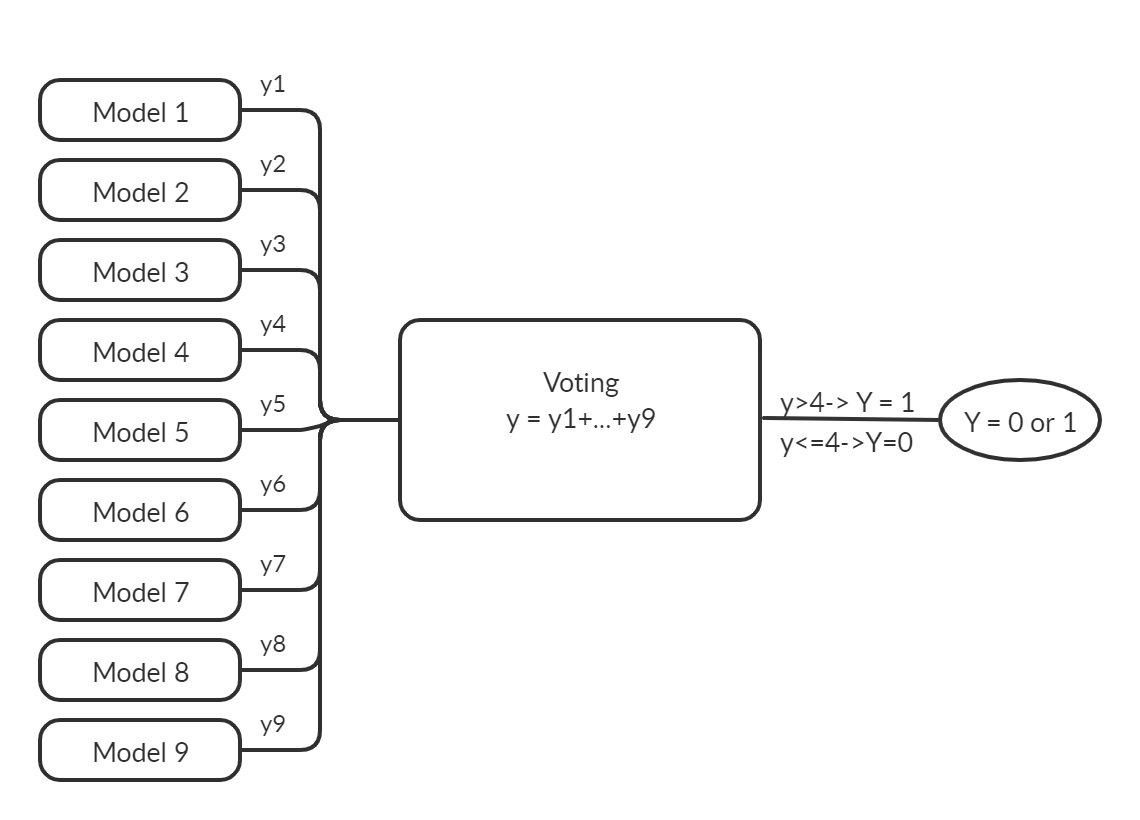
\includegraphics[width=0.6\linewidth]{voting.png} \caption{Ensemble με ψηφοφορία για 9 μοντέλα για συγκεκριμένο κατώφλι t}
      \label{figure:voting}    
\end{figure}
  
  



\section{Επιπλέον Πειράματα}
\label{sec:5.4}
Σε αυτή την παράγραφο θα γίνει αναφορά σε ορισμένα πειράματα  που πραγματοποιήθηκαν με σκοπό τη βελτίωση των αποτελεσμάτων, ωστόσο έδωσαν παρόμοια ή κατώτερα αποτελέσματα. Κρίνεται σκόπιμο να γίνει αναφορά σε αυτά τα πειράματα, ώστε να υπάρχει η γνώση της μη αποτελεσματικότητα τους.


\subsection{Αλλαγή από RGB σε άλλους Xρωματικούς Xώρους}
\label{subsec:5.4.1}
Δοκιμάστηκε ο μετασχηματισμός των εικόνων από RGB στους χρωματικούς χώρους YUV και Lab. Ο χρωματικός χώρος YUV προέρχεται από γραμμικό μετασχηματισμό των RGB  καναλιών όποτε πιθανότατα η μετατροπή αυτή δεν προσφέρει κάποια καινούργια πληροφορία στο νευρωνικό. Αντίθετα, ο χρωματικός χώρος Lab δεν προέρχεται από γραμμικό μετασχηματισμό των RGB καναλιών και ίσως θα μπορούσε να αποδώσει καλύτερα την πληροφορία των εικόνων.  Όπως αποδείχθηκε  πειραματικά η μετατροπή των εικόνων στους παραπάνω χρωματικούς χώρους έδωσε παρόμοια, με τον χρωματικό χώρο RGB, αποτελέσματα.

\subsection{Μετασχηματισμός Clahe}
\label{subsec:5.4.2}
Για την ενίσχυση της τοπικής αντίθεσης των εικόνων δοκιμάστηκε ο μετασχηματισμός Contrast Limited Adaptive histogram equalization(Clahe), μία παραλλαγή του μετασχηματισμού Adaptive histogram equalization, με μέγεθος γειτονιάς 8x8\cite{clahe}. Ο μετασχηματισμός εφαρμόστηκε με τις εξής μορφές: 1. Εφαρμογή μετασχηματισμού  σε κάθε ένα από τα RGB κανάλια ξεχωριστά, 2.  Μετασχηματισμός των εικόνων σε YUV χρωματικό χώρο, εφαρμογή Clahe στο κανάλι Y και επιστροφή στο RGB χρωματικό χώρο  3.  Μετασχηματισμός των εικόνων σε Lab χρωματικό χώρο, εφαρμογή Clahe στο κανάλι L και επιστροφή στο RGB χρωματικό χώρο. 

Επιπλέον, δοκιμάστηκε αντί των 3 καναλιών RGB χρήση 3 καναλιών με το πρώτο κανάλι να περιέχει το μετασχηματισμό Clahe της ασπρόμαυρης εικόνας, το δεύτερο εικόνες εντροπίας και το τρίτο το Y κανάλι από το μετασχηματισμό YUV. Οι εικόνες εντροπίας υπολογίζονται αφού πρώτα μετατραπεί η εικόνα σε κλίμακα του γκρι (grayscale) και στη συνέχεια αντικατασταθεί κάθε εικονοστοιχείο με την τιμή της εντροπίας σε μία γειτονιά του εικονοστοιχείου.

\subsection{Αύξηση Δεδομένων πριν την Είσοδο στο Νευρωνικό}
\label{subsec:5.4.3}
Δοκιμάστηκε και η αύξηση δεδομένων πριν δοθούν στο νευρωνικό ώστε να υπάρχει ίδιος αριθμός εικόνων σε κάθε κλάση. Έτσι στην κλάση rDR που υπάρχουν πολύ λιγότερες εικόνες παράχθηκαν νέες εικόνες  από τις ήδη υπάρχουσες. Οι νέες εικόνες παράχθηκαν με αλλαγή της φωτεινότητας, του κορεσμού, της απόχρωσης και της αντίθεσης των εικόνων της κλάσης rDR. Από αυτή τη διαδικασία o  χρόνος εκπαίδευσης αυξήθηκε αρκετά χωρίς ωστόσο να βελτιωθούν τα αποτελέσματα. Να σημειωθεί ότι και σε αυτό το πείραμα έγινε αύξηση δεδομένων κατά τη διάρκεια της εκπαίδευσης.

\subsection{Χρήση Ασπρόμαυρης Μάσκας}
\label{subsec:5.4.4}
Δοκιμάστηκε η χρήση δύο ασπρόμαυρων μασκών για τις δύο μορφές εικόνων. Η μία μάσκα περιείχε ολόκληρο τον αμφιβληστροειδή ενώ η δεύτερη είχε κομμένο το πάνω και κάτω μέρος κατά αναλογία με τις εικόνες του συνόλου δεδομένων Kaggle. Στην εικόνα \ref{figure:bl} παρουσιάζονται οι δύο μάσκες. 


\begin{figure}[!h]
\centering
\begin{subfigure}{.5\textwidth}
  \centering
  
\includegraphics[scale=0.5]{bl.png}
  \caption{Μάσκα 1}
  \label{fig:bl1}
\end{subfigure}
\qquad
\begin{subfigure}{.5\textwidth}
  \centering
  
\includegraphics[scale=0.5]{bl2.png}
  \caption{Μάσκα 2}
  \label{fig:bl2}
\end{subfigure}
\caption{Μάσκες}
\label{figure:bl}
\end{figure}

Κάθε εικόνα πολλαπλασιάστηκε με την αντίστοιχη μάσκα και το αποτέλεσμα έδωσε μία πιο σταθερή δομή στις εικόνες και ένα ομοιόμορφο μαύρο φόντο για τις εικόνες που είχαν εικονοστοιχία διάφορα του [0,0,0] στο φόντο. Με την εφαρμογή των παραπάνω μασκών χάνεται ένα κομμάτι της πληροφορίας της εικόνας το οποίο όμως δεν θεωρείται σημαντικό καθώς  η ασθένεια δεν εντοπίζεται συνήθως στα άκρα του αμφιβληστροειδούς. Κάποια ενδεικτικά δείγματα των εικόνων που παρήχθησαν παρουσιάζονται στην \ref{figure:stable}. Η εφαρμογή των μασκών στις εικόνες δεν έδωσε καλύτερα αποτελέσματα.

\begin{figure}[!h]
    \centering
      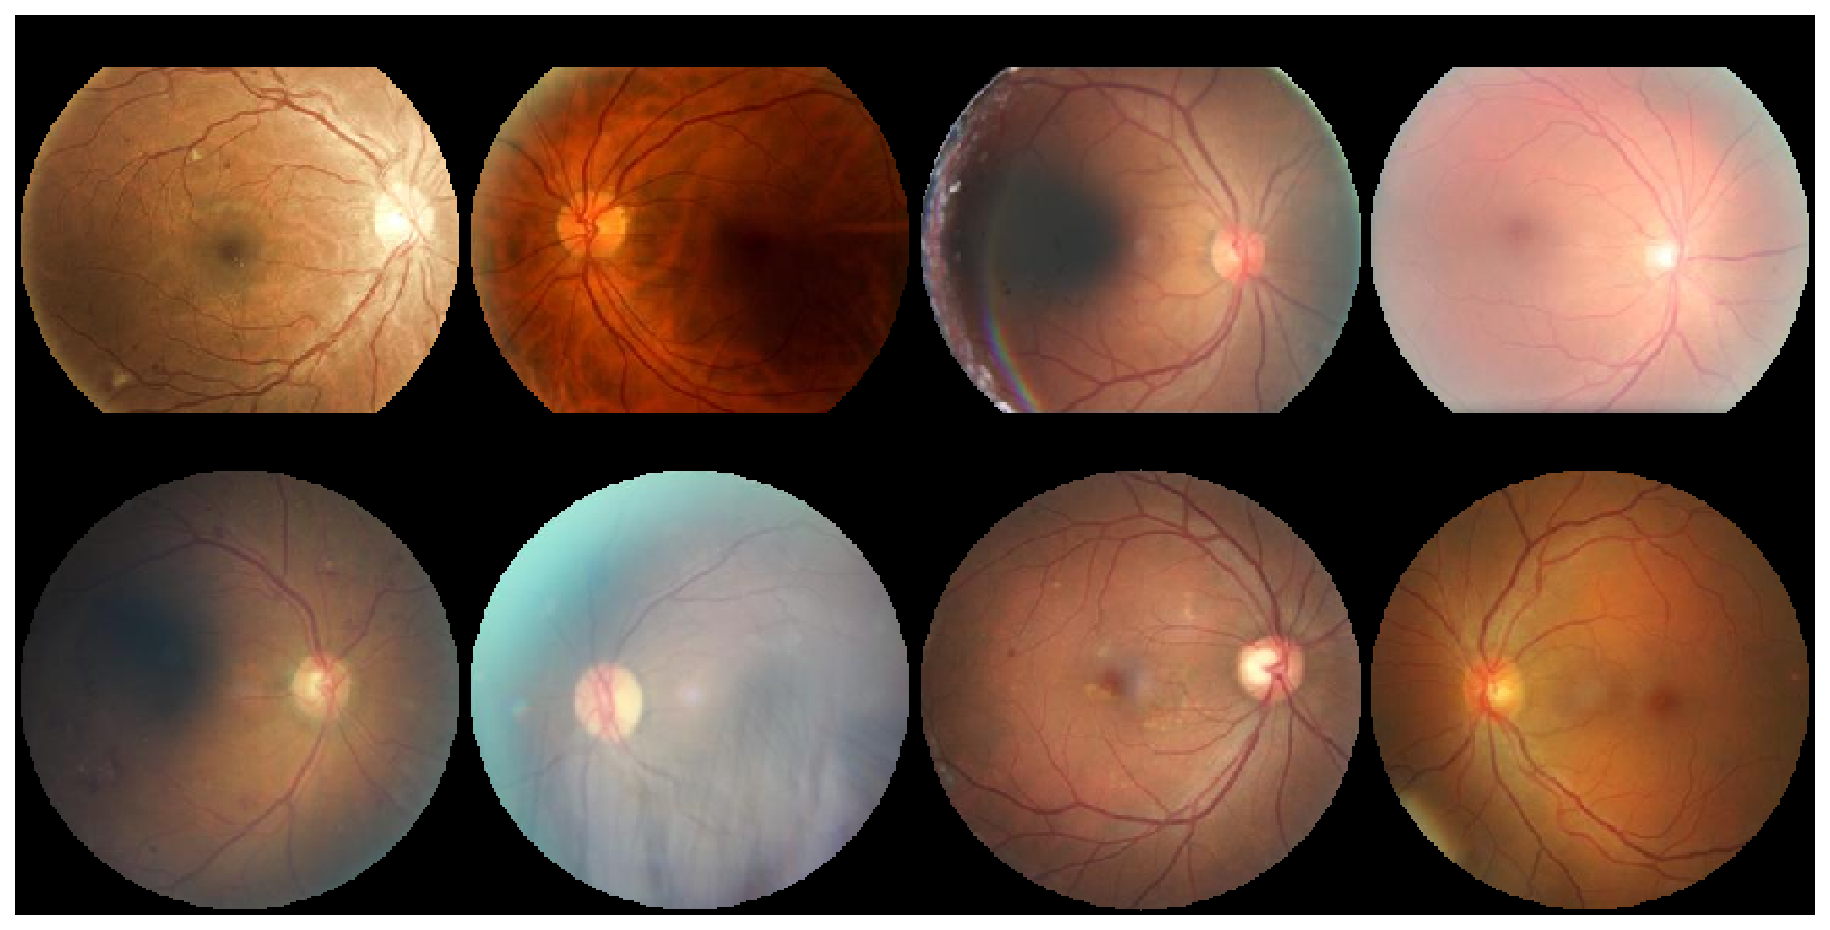
\includegraphics[width=1\linewidth]{stable.pdf} \caption{Εφαρμογή μασκών στο σύνολο δεδομένων Kaggle}
\label{figure:stable}  
\end{figure}

\subsection{Αλλαγή Δομής InceptionV3 με Χρήση Ασπρόμαυρης Μάσκας}
\label{subsec:5.4.5}

Στις εικόνες που δίνονται ως είσοδο στο νευρωνικό, όλη η πληροφορία του προβλήματος περιέχεται στον αμφιβληστροειδή ενώ το εξωτερικό φόντο δεν παρέχει καμία πληροφορία. Βάση αυτής της σκέψης πραγματοποιήθηκε μία μετατροπή στο νευρωνικού Inception V3. Η μετατροπή αυτή περιείχε  τον πολλαπλασιασμό των χαρτών χαρακτηριστικών με μία ασπρόμαυρη μάσκα με μηδενισμένα τα εικονοστοιχεία του φόντο και με τιμή ένα στα εικονοστοιχεία στην περιοχή του αμφιβληστροειδούς. Παρακάτω θα δοθούν κάποιες επιπλέον λεπτομέρειες για τη μέθοδο.

Έγινε χρήση εικόνων τεσσάρων καναλιών αντί τριών. Τα τρία  κανάλια περιείχαν την rgb εικόνα ενώ στο τέταρτο τοποθετήθηκε μία ασπρόμαυρη μάσκα. Έγινε χρήση 2 ειδών μάσκας: η μία μάσκα περιείχε ολόκληρο τον αμφιβληστροειδή ενώ η δεύτερη είχε κομμένο το πάνω και κάτω μέρος κατά αναλογία με τις εικόνες του συνόλου δεδομένων Kaggle.  Καθώς το Keras περιορίζει τον τύπο δεδομένων και τον αριθμό καναλιών που μπορεί να δεχτεί ως είσοδο το εκάστοτε νευρωνικό δίκτυο, για να είναι δυνατή η αποθήκευση πληροφορίας σε τέσσερα κανάλια έγινε χρήση rgba εικόνων. Οι  rgba εικόνες περιέχουν στο τρία πρώτα κανάλια τις εικόνες rgb και στο τέταρτο κανάλι τις τιμές που καθορίζουν την αδιαφάνεια ενός χρώματος, 0 (πλήρως διαφανές) και 1.0 (πλήρως αδιαφανές). Ένα δείγμα των εικόνων που δημιουργήθηκαν παρουσιάζονται στη εικόνα \ref{figure:rgba}. Να σημειωθεί ότι η χρήση εικόνων rgba έγινε για πρακτικούς λόγους καθώς έπρεπε να βρεθεί τρόπος να δοθούν ως είσοδο στο νευρωνικό εικόνες με τέσσερα κανάλια.

\begin{figure}[!h]
\centering
\begin{subfigure}{.5\textwidth}
  \centering
  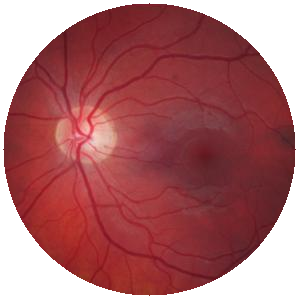
\includegraphics[scale=0.5]{rgba.png}
  \caption{Δείγμα 1}
  \label{fig:rgba1}
\end{subfigure}
\qquad
\begin{subfigure}{.5\textwidth}
  \centering
  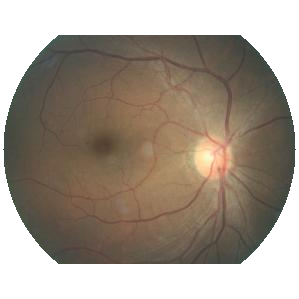
\includegraphics[scale=0.5]{rgb2.png}
  \caption{Δείγμα 2}
  \label{fig:rgba2}
\end{subfigure}
\caption{Παραδείγματα RGBA εικόνων}
\label{figure:rgba}
\end{figure}

Το τέταρτο κανάλι χρησιμοποιήθηκε ως μάσκα στους παραγόμενους χάρτες χαρακτηριστικών. Ουσιαστικά μετά από κάθε συνελικτικό επίπεδο, μέχρι τη μείωση σε 8x8 χάρτες χαρακτηριστικών, εφαρμόζονταν πολλαπλασιασμός κάθε χάρτη χαρακτηριστικών με τη μάσκα. Για να είναι δυνατός ο πολλαπλασιασμός οι διαστάσεις της αρχικής μάσκας μειωνώταν ανάλογα με τις διαστάσεις των χαρτών χαρακτηριστικών. 

Γενικά, το νευρωνικό Inception V3 περιέχει συνεχή μείωση των διαστάσεων των χαρτών χαρακτηριστικών με παράλληλη αύξηση των καναλιών τους, το οποίο υλοποιείται με συνελικτικά επίπεδα και επίπεδα υποδειγματοληψίας. Στα τελευταία επίπεδα παράγονται 17x17 χάρτες χαρακτηριστικών και στη συνέχεια γίνεται η τελική μείωση σε 8x8 χάρτες χαρακτηριστικών. Αποφασίστηκε η μη χρήση μάσκας στους 8x8 χάρτες χαρακτηριστικων καθώς οι διαστάσεις ήταν πολύ μικρές και θα μπορούσε να χαθεί χρήσιμη πληροφορία στα άκρα.



Για να γίνουν τα παραπάνω καθώς το Inception V3 του Keras καλείται σαν συνάρτηση και δεν επιδέχεται αλλαγές στη δομή του, ο κώδικας του Inception V3 κατέβηκε τοπικά και μετά από κάποιες αλλαγές ήταν δυνατή η χρήση του ως τοπική συνάρτηση τους συστήματος. Στη συνέχεια προστέθηκαν όλες οι αλλαγές που περιγράφηκαν παραπάνω και το σύστημα ήταν έτοιμο να τρέξει. Το σύστημα δεν παρουσίασε βελτιωμένα αποτελέσματα. Στην εικόνα \ref{figure:masked} παρουσιάζονται κάποιοι χάρτες χαρακτηριστικών μετά την εφαρμογή της μάσκας. Όπως είναι φανερό το φόντο δεν έχει καμία ενεργοποιημένη περιοχή.

\begin{figure}[!h]
    \centering
      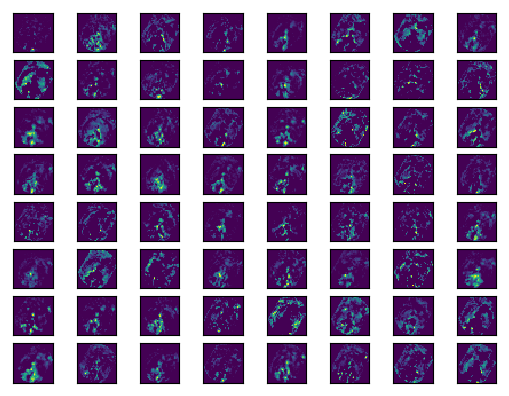
\includegraphics[width=0.8\linewidth]{FMmask.png} \caption{Χάρτες χαρακτηριστικών μετά την εφαρμογή μάσκας}
\label{figure:masked}  
\end{figure}




\chapter{ Μετρικές}
\label{chap:6}

\section{Αξιολόγηση κατά την Εκπαίδευση}
\label{sec:6.1}

Κατά τη διάρκεια της εκπαίδευσης έγινε χρήση δύο μετρικών, της Binary Cross-Entropy loss και της Ακρίβειας(Αccuracy). Οι 2 παραπάνω μετρικές χρησιμοποιήθηκαν για την αξιολόγηση του μοντέλου κατά τη διάρκεια της εκπαίδευσης για το σύνολο εκπαίδευσης και το σύνολο επικύρωσης. 

\subsection{Binary Cross-Entropy loss}
\label{subsec:6.1.1}
H Binary Cross-Entropy loss είναι μία συνάρτηση που χρησιμοποιείται σε δυαδικά προβλήματα και μετράει την επίδοση ενός μοντέλου ταξινόμησης του οποίου η έξοδος είναι μία πιθανότητα στο διάστημα [0,1]. Η μετρική αυξάνεται όσο η προβλεπόμενη 
πιθανότητα αποκλίνει από την πραγματική κλάση που ανήκει. Για ένα μοντέλο που πάντα προβλέπει σωστά, η τιμή της μετρικής θα είναι $0$. Για κάποιο δεδομένο εισόδου η μετρική ορίζεται από την εξίσωση:

\begin{equation}
loss = -ylog(p) - (1-y) log(1 -p)
\end{equation}

όπου y η πραγματική κλάση του δεδομένου εισόδου με τιμή $0$ ή $1$ και p η πιθανότητα που προέβλεψε το μοντέλο. Αν για παράδειγμα μία είσοδος άνηκε στην κλάση $0$ και η πρόβλεψη του μοντέλου ήταν $0.1$, τότε το σφάλμα θα ήταν 0.045. Αντίθετα αν η πρόβλεψη ήταν $0.4$, τότε το σφάλμα θα ήταν $0.22$, δηλαδή πολύ μεγαλύτερο. Στην εικόνα \ref{figure:cross} παρουσιάζεται η συνάρτηση Binary Cross-Entropy loss για εισόδους με πραγματική τιμή $1$. Όταν η πρόβλεψη του μοντέλου είναι κοντά στο $1$ το σφάλμα μηδενίζεται, αντίθετα για προβλέψεις κοντά στο $0$ το σφάλμα απειρίζεται. Να σημειωθεί ότι η μετρική για όλα τα δεδομένα υπολογίζεται ως ένας μέσος όρος όλων των σφαλμάτων των δεδομένων. Κατά την διάρκεια της εκπαίδευσης η συγκεκριμένη μετρική χρησιμοποιήθηκε ως ένα εποπτικό μέσο για την επίδοση του μοντέλου. Στο τέλος κάθε εποχής υπολογίζονταν το σφάλμα  για το σύνολο εκπαίδευσης και το σύνολο επικύρωσης. Επιπλέον, το μοντέλο με το μικρότερο σφάλμα Binary Cross-Entropy για τα δεδομένα επικύρωσης σε μία εποχή, αποθηκεύονταν ως το τελικό μοντέλο του πειράματος. 

\begin{figure}[!h]
    \centering
      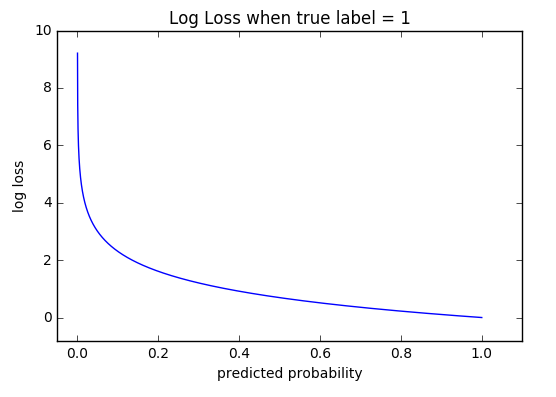
\includegraphics[width=0.6\linewidth]{crossentropy.png} \caption{Συνάρτηση Binary Cross-Entropy loss για δεδομένα της κλάσης 1}
\label{figure:cross}    
\end{figure}
  
  
\subsection{Ακρίβεια(Accuracy)}
\label{subsec:6.1.2}
Η ακρίβεια ορίζεται από τον τύπο \ref{eq:acc}. Κατά την διάρκεια της εκπαίδευσης χρησιμοποιήθηκε ως ένα εποπτικό μέσο για την επίδοση του μοντέλου. Στο τέλος κάθε εποχής υπολογίζονταν η ακρίβεια για το σύνολο εκπαίδευσης και το σύνολο επικύρωσης.

\begin{equation} \label{eq:acc}
Accuracy = \frac{TP+TN}{TP+TN+FP+FN}
\end{equation}



\section{Μετρικές Αξιολόγηγης Μοντέλου}
\label{sec:6.2}



\subsection{TPR, TNR, FPR, FNR}
\label{subsec:6.2.1}

\paragraph{True Positive Rate - Ευαισθησία}
Η μετρική  True Positive Rate ή αλλιώς Ευαισθησία(Sensitivity) εκφράζει την πιθανότητα μία εικόνα με rDR, να ταξινομηθεί σωστά στην κλάση rDR.

\begin{equation} \label{eq:6.9}
TPR = \frac{TP}{TP + FN}
\end{equation}

\paragraph{False Negative Rate}
Η μετρική  False Negative Rate εκφράζει την πιθανότητα μια εικόνα με rDR, να ταξινομηθεί στην κλάση no rDR. 

\begin{equation} \label{eq:6.12}
TNR = \frac{FN}{TP + FN}
\end{equation}

\paragraph{True Negative Rate - Εξειδίκευση}

Η μετρική  True Negative Rate ή αλλιώς Εξειδίκευση(Specificity) εκφράζει την πιθανότητα μια εικόνα χωρίς rDR, να ταξινομηθεί σωστά στην κλάση no rDR. 

\begin{equation} \label{eq:6.11}
TNR = \frac{TN}{FP + TN}
\end{equation}


\paragraph{False Positive Rate}
Η μετρική  False Positive Rate εκφράζει τη πιθανότητα μία εικόνα χωρίς rDR, να ταξινομηθεί λάθος στην κλάση rDR. 


\begin{equation} \label{eq:6.10}
FPR = \frac{FP}{FP + TN}
\end{equation}



\par
όπου:

True Positive(TP) = αριθμός εικονων με rDR που ταξινομήθηκαν στην κλάση rDR.

True Negative(TN) = αριθμός εικόνων χωρίς rDR που ταξινομήθηκαν στην κλάση no rDR.

False Positive(FP) = αριθμός εικόνων χωρίς rDR που ταξινομήθηκαν στην κλάση rDR.

False Negative(FN) =  αριθμός εικονων με rDR που ταξινομήθηκαν στην κλάση no rDR.



\subsection{Roc curve - Area Under the Curve(AUC)}
\label{subsec:6.2.2}
Το τελευταίο επίπεδο του νευρωνικού  περιέχει ένα νευρώνα και η έξοδος του δίνει την πιθανότητα μία εικόνα να ανήκει στην κλάση rDR. Για να ταξινομηθεί μία εικόνα σε μία κλάση πρέπει να τεθεί ένα κατώφλι πάνω από το οποίο τα δείγματα θα ταξινομούνται στην κλάση rDR, ενώ κάτω από αυτό στην κλάση no rDR. Αλλάζοντας αυτό το κατώφλι και υπολογίζοντας τα \textit{False Positive rate}  και  \textit{True Positive rate} σχηματίζεται η καμπύλη ROC. Πιο συγκεκριμένα, στον οριζόντιο άξονα τοποθετείται το FPR ενώ στο κατακόρυφο το TPR, καθώς τα FPR, TPR είναι πιθανότητες οι άξονες εκτείνονται στο $[0,1]$. Ένα παράδειγμα ROC καμπύλης δίνεται στην εικόνα \ref{figure: AUC}. 

\begin{figure}[!h]
    \centering
      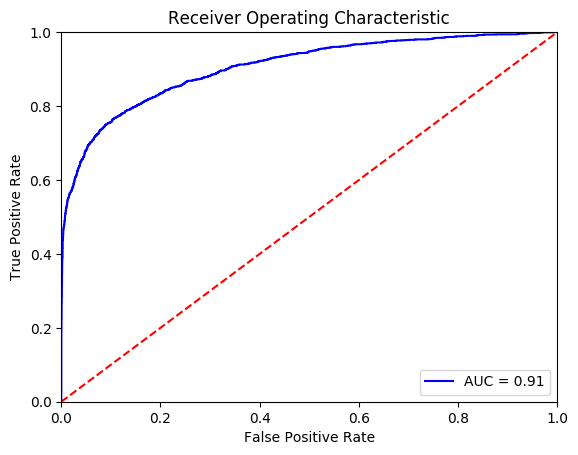
\includegraphics[width=0.6\linewidth]{AUC.png} \caption{ROC - AUC}
       \label{figure: AUC}    
  \end{figure}



Η μετρική Area Under the Curve(AUC) υπολογίζεται από το εμβαδόν που βρίσκεται κάτω από την καμπύλη ROC και τους άξονες και παίρνει τιμές στο [0,1]. Η μετρική AUC αποτελεί ένα μέτρο της διαχωρισιμότητας μεταξύ των κλάσεων. Η σημασία της θα γίνει καλύτερα αντιληπτή μέσω της εικόνας \ref{figure:aucExample} \cite{ROC}. Έστω ότι το σύνολο των πράσινων και κόκκινων κουκίδων αποτελεί το σύνολο ελέγχου. Οι κόκκινες κουκίδες παριστάνουν δείγματα της κλάσεις no rDR ενώ οι πράσινες ανήκουν στην κλάση rDR.
Ο άξονας κάτω από τις κουκίδες αναπαριστά την πρόβλεψη του μοντέλου για κάθε δείγμα.  

Αν τεθεί ως τιμή  κατωφλίου η τιμή του άξονα πριν το σημείο εμφάνισης του πρώτου πρασίνου(από αριστερά προς τα δεξιά), θα ταξινομηθούν λανθασμένα τέσσερα κόκκινα δείγματα της κλάσης no rDR στη κλάση rDR. Αν τεθεί ως τιμή κατωφλίου η τιμή του άξονα πριν το σημείο εμφάνισης του επόμενου δείγματος, τα δείγματα που θα ταξινομηθούν λάθος, θα είναι πέντε (ένα πράσινο και τέσσερα κόκκινα). Με την ίδια λογική μετατοπίζοντας το κατώφλι πριν το επόμενο δείγμα, θα συμβούν τέσσερις λάθος ταξινομήσεις (τρία κόκκινα και ένα πράσινο). Όπως είναι φανερό, με κανένα κατώφλι δεν δύναται να επιτευχθεί σωστή ταξινόμηση όλων των δειγμάτων του συνόλου ελέγχου, δηλαδή τέλειο διαχωρισμό κλάσεων και AUC =1. Μετά την παραπάνω ανάλυση μπορεί να γίνει εύκολα κατανοητό ότι η μετρική AUC αναπαριστά την πιθανότητα μία οποιαδήποτε εικόνα με rDR(πράσινες κουκίδες) να βρίσκεται στα δεξιά, μιας οποιασδήποτε εικόνας χωρίς rDR(κόκκινες κουκίδες) στον άξονα με τις προβλέψεις. 

\begin{figure}[!h]
    \centering
      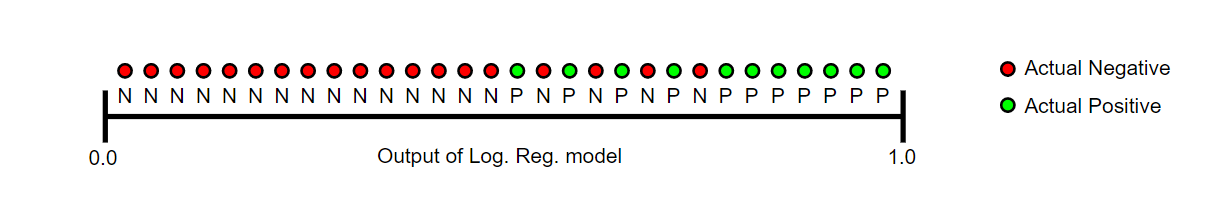
\includegraphics[width=1\linewidth]{auc_example.PNG} \caption{Αναπαράσταση προβλέψεων για ενα σύνολο δεδομενων πάνω σε άξονα}
       \label{figure:aucExample}    
  \end{figure}
  
  
  
\section{Υπολογισμός σημείων}
\label{sec:6.3}


\subsection{Σημείο υψηλής Ευαισθησίας}
\label{subsec:6.3.1}




Για να βρεθεί το σημείο υψηλής Ευαισθησίας(High Sensitivity), ορίζεται η μικρότερη αποδεκτή τιμή  Ευαισθησίας που ικανοποιεί τη συνθήκη για υψηλή Ευαισθησία. Έστω ότι μία εφαρμογή απαιτεί Ευαισθησία τουλάχιστον 0.9, για τιμές 0.9 και άνω, υπολογίζεται το άθροισμα (Ευαισθησία  + Εξειδίκευση) για τα διάφορα κατώφλια(thresholds). Σημείο υψηλής Ευαισθησίας ορίζεται το σημείο που μεγιστοποιεί το άθροισμα και περιγράφεται από την τριπλέτα [Sensitivity, Specificity, thresholds]. Στην \ref{eq:6new} παρουσιάζεται η μαθηματική περιγραφή για την εύρεση σημείου υψηλής Ευαισθησίας. 




\begin{equation} \label{eq:6new}
maximaze(Sens_{t} + Spec_{t}),~ για~ Sens_{t}>Sens_{min}
\end{equation}

όπου τα $Sens_{t}$ και $Spec_{t}$ αποτελούν τις τιμές Ευαισθησίας και Εξειδίκευσης αντίστοιχα σε ένα κατώφλι $t$ και η $Sens_{min}$ την ελάχιστη αποδεκτή τιμή της Ευαισθησίας.


\subsection{Σημείο υψηλής Εξειδίκευσης}
\label{subsec:6.3.2}
Η ίδια διαδικασία με την εύρεση σημείου υψηλής Ευαισθησίας ακολουθείται και για την εύρεση σημείου υψηλής Εξειδίκευσης οπότε παραλείπεται η περεταίρω ανάλυση. Στην \ref{eq:6bnew} παρουσιάζεται η μαθηματική περιγραφή για την εύρεση σημείου υψηλής Εξειδίκευσης. 


\begin{equation} \label{eq:6bnew}
maximaze(Sens_{t} + Spec_{t}),~ για~ Spec_{t}>Spec_{min}
\end{equation}

όπου τα $Sens_{t}$ και $Spec_{t}$ αποτελούν τις τιμές Ευαισθησίας και Εξειδίκευσης αντίστοιχα σε ένα κατώφλι $t$ και η $Spec_{min}$ την ελάχιστη αποδεκτή τιμή της Εξειδίκευσης.



\subsection{Βέλτιστο σημείο}
\label{subsec:6.3.3}
Ως βέλτιστο σημείο ορίζεται το σημείο στο οποίο μεγιστοποιείται το άθροισμα (Ευαισθησία + Εξειδίκευση). Καθώς το μοντέλο εκπαιδεύτηκε δίνοντας ίδιο βάρος στις δύο κλάσεις, το σημείο θεωρητικά παρουσιάζει σχετικά καλές τιμές στην πρόβλεψη και τον 2 κλάσεων(rdr/no rdr). Στην \ref{eq:6c} παρουσιάζεται η μαθηματική περιγραφή για την εύρεση βέλτιστου σημείου.


\begin{equation} \label{eq:6c}
maximaze(Sens_{t} + Spec_{t})
\end{equation}


  



\thispagestyle{plain}
\chapter{ Αποτελέσματα και Μελλοντικές Επεκτάσεις}
\label{chap:7}



\section{Οπτικοποίηση με Grad-CAM}
\label{chap:7.1}

Η οπτικοποίηση των περιοχών που εστιάζει το νευρωνικό έχει διττό ρόλο στο πρόβλημα καθώς δίνει πληροφορίες για τη λειτουργία του νευρωνικού ενώ συγχρόνως αποτελεί ένα κατευθυντήριο μέσο για τον ιατρό στη διαδικασία της διάγνωσης, καθώς επισημαίνει τις περιοχές που βρίσκεται η ασθένεια. 


\subsection{Μέθοδος Grad-CAM} 
\label{sec:7.1.1}
Gradient class activation maps(Grad-CAM) είναι μία τεχνική οπτικοποίησης για τα βαθιά συνελικτικά δίκτυα \cite{Ramprasaath}. Παρακάτω παρουσιάζεται η διαδικασία που ακολουθείται μέχρι την τελική οπτικοποίηση.
Αρχικά, υπολογίζεται  η κλίση της πρόβλεψης $y^c$ της κλάσης c (πριν την εφαρμογή της συνάρτησης softmax), ως προς τους χάρτες χαρακτηριστικών $ A^k $ κάποιου συνελικτικού επιπέδου( $\frac{\partial y^c}{\partial A^k }$). Είναι δυνατόν να επιλεχθεί οποιοδήποτε συλλεκτικό επίπεδο, ωστόσο προτιμάτε το τελευταίο καθώς περιέχει την περισσότερη πληροφορία.
 Έπειτα, εφαρμόζεται καθολική υποδειγματοληψία για να υπολογιστούν τα βάρη $a_{k}^c$ για κάθε χάρτη χαρακτηριστικών. Το βάρος $a_{k}^c$   αποδίδει τη σημασία του k χάρτη χαρακτηριστικών για την κλάση c. Η παραπάνω διαδικασία αυτή παρουσιάζεται στην εξίσωση \ref{eq:7.10}.

\begin{equation} \label{eq:7.10}
a_{k}^c =  \frac{1}{Z} \sum_{i}  \sum_{j} \frac{\partial y^c}{\partial A_{ij}^k }
\end{equation}

Τέλος, ο κάθε χάρτης χαρακτηριστικών πολλαπλασιάζεται με το αντίστοιχο βάρος του και στη συνέχεια εφαρμόζεται συνάρτηση Ανόρθωσης. Επιλέγεται η εφαρμογή της συνάρτησης Ανόρθωσης γιατί χρήσιμα είναι τα χαρακτηριστικά που έχουν θετική επιρροή στην κλάση ενδιαφέροντος όπως εικονοστοιχεία  που η ένταση τους πρέπει να αυξηθεί για να αυξηθεί η $y^{c}$. Χωρίς τη συνάρτηση Ανόρθωσης είναι πολύ πιθανό να επισημανθούν στοιχεία άσχετα με την επιθυμητή κλάση.

\begin{equation} \label{eq:7.11}
L_{GradCAM}^c =  ReLU(\sum_{k} a_{k}^c  A^k)
\end{equation}

 Στην εικόνα \ref{fig:fm1} παρουσιάζονται κάποιοι από τους  χάρτες χαρακτηριστικών, για είσοδο μία τυχαία εικόνα του συνόλου ελέγχου ενός συνελικτικού επιπέδου 35x35 του νευρωνικού και στην \ref{fig:fm2}  κάποιοι από τους χάρτες χαρακτηριστικών του τελευταίου συνελικτικού επιπέδου 8x8 για την ίδια εικόνα. Είναι φανερό ότι οι χάρτες χαρακτηριστικών 35x35 δείχνουν με πολύ μεγαλύτερη ακρίβεια τις περιοχές ενεργοποίησης του μοντέλου ωστόσο οι χάρτες χαρακτηριστικών του τελευταίου συνελικτικού επιπέδου περιέχουν περισσότερη πληροφορία σχετικά με την ενεργοποίηση των κλάσεων. 




\begin{figure}[!h]
\centering
\begin{subfigure}{.5\textwidth}
  \centering
  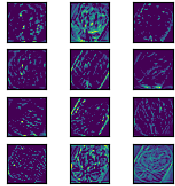
\includegraphics[scale=1.05]{f1.png}
  \caption{Χάρτες Χαρακτηριστικών 35x35}
  \label{fig:fm1}
\end{subfigure}
\begin{subfigure}{.5\textwidth}
  \centering
  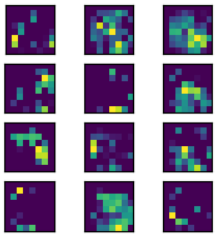
\includegraphics[scale=1]{f2.PNG}
  \caption{Χάρτες Χαρακτηριστικών 8x8}
  \label{fig:fm2}
\end{subfigure}
\caption{Όπτικοποίηση των Χαρτών Χαρακτηριστικών για μία τυχαία εικόνα του συνόλου ελέγχου}
\label{figure:fm}
\end{figure}




\subsection{ Αποτελέσματα οπτικοποίησης Νευρωνικού} 
\label{sec:7.1.3}

Όπως εξηγήθηκε και πιο πάνω οι περιοχές στις οποίες εστιάζει το νευρωνικό για να ταξινομήσει μια εικόνα στην κλάση rDR, εξάγονται από χάρτες χαρακτηριστικών διαστάσεων $8x8$. H παραπάνω μέθοδος μετά τη διαδικασία που εξηγήθηκε παραπάνω παράγει μία εικόνα διαστάσεων $8x8$, η οποία περιέχει τις περιοχές ενεργοποίησης της κλάσης rDR.
Έτσι, όταν γίνεται υπερδειγματοληψία στην  $8x8$ εικόνα, για αύξηση των διαστάσεων της εικόνας σε $299x299$, μία περιοχή 8x8 στην αρχική εικόνα, θα αντιστοιχίζεται σε μια περιοχή 37x37 στην νέα εικόνα. Με την παραπάνω ανάλυση γίνεται φανερό το πρόβλημα που αντιμετωπίζει η μέθοδος στον ακριβή προσδιορισμό των περιοχών της ασθένειας. 

Όπως θα γίνει φανερό και από τα παραδείγματα που θα παρουσιαστούν παρακάτω, οι περιοχές ενδιαφέροντος συνήθως εντοπίζονται σε μεγαλύτερη επιφάνεια από τα πραγματικά συμπτώματα. Επιπλέον, περιοχές που υπάρχουν πολλά συμπτώματα, παρουσιάζονται στην εικόνα ως μία ενιαία μεγάλη περιοχή. Τέλος, λόγω  της μικρής διάστασης των χαρτών χαρακτηριστικών, κάποιες φορές στις περιοχές ενεργοποίησης περιλαμβάνεται και το φόντο της εικόνας. Παρακάτω, θα σχολιαστούν κάποια παραδείγματα οπτικοποίησης.

Για τη γραφική αναπαράσταση των περιοχών ενδιαφέροντος έγινε χρήση Heat map. Ουσιαστικά, οι περιοχές ενδιαφέροντος εντοπίζονται με επίκεντρο στο πορτοκαλί χρώμα και φθίνουν μέχρι το κυανό. Οι περιοχές με μπλε χρώμα θεωρούνται μη σημαντικές για την ταξινόμηση στην κλάση rDR.

Στην εικόνα \ref{figure:viz1n} παρατηρούνται μία πληθώρα συμπτωμάτων, τα οποία ανιχνεύει το μοντέλο. Μεγαλύτερη βάση δίνεται στην περιοχή με πιο έντονα τα συμπτώματα της ασθένειας, η οποία χρωματίζεται με πορτοκαλί. Μεγάλη επιφάνεια καταλαμβάνει το κυανό χρώμα που αποτελεί σημείο ενδιαφέροντος, ωστόσο με μικρότερη  επιρροή για την τελική απόφαση αφού στην περιοχή αυτή υπάρχουν κάποια διάσπαρτα εξιδρώματα ενώ στον οπτικό δίσκο παρατηρείται ανάπτυξη νέων αγγείων.

Στην εικόνα \ref{figure:viz2n} τα χαρακτηριστικά είναι πολύ πιο ήπια για τον παρατηρητή ωστόσο το νευρωνικό ανιχνεύει 3 περιοχές ενδιαφέροντος, που περιέχουν βαμβακόμορφες κηλίδες και ίσως κάποια νεοαγγεία. Στη συγκεκριμένη εικόνα γίνεται φανερό ότι το μοντέλο μπορεί και εντοπίζει και πιο ήπια συμπτώματα που δεν καταλαμβάνουν πολύ χώρο.

Στην εικόνα \ref{figure:viz3n} υπάρχει μία περιοχή με πολλά σκληρά εξιδρώματα την οποία εντοπίζει το νευρωνικό. Στη περιοχή αυτή φαίνονται πολύ έντονα τα εξιδρώματα τα οποία αποτελούν κύριο σύμπτωμα της ασθένειας ωστόσο εξιδρώματα απαντώνται σε όλη την εικόνα σε ηπιότερη μορφή . Το νευρωνικό μπορεί να έχει ανιχνεύσει και αυτές τις περιοχές ωστόσο η επιρροή τους για την τελική απόφαση να είναι αμυδρή σε σχέση με την επιρροή της μεγάλης περιοχής και για αυτό να μην αναπαριστάται στο Heatmap. 

Η εικόνα \ref{figure:viz4n} επισημαίνονται δύο ενωμένες περιοχές ενδιαφέροντος με τη μία πάνω και δεξιά από τον οπτικό δίσκο και την άλλη κάτω και δεξιά. Η πάνω και δεξιά περιοχή περιλαμβάνει μία  βαμβακόμορφη κηλίδα ενώ στην κάτω δεξιά εντοπίζεται μια  βαμβακόμορφη κηλίδα μεγαλύτερων διαστάσεων και ένα αιμάτωμα. Στην οπτικοποίηση επισημαίνεται με πιο έντονο χρωματισμό ότι η κάτω περιοχή αποτελεί πιο έντονο σύμπτωμα της ασθένειας καθώς η  βαμβακόμορφη κηλίδα καταλαμβάνει μεγαλύτερη επιφάνεια.


%\begin{figure}[!h]
%    \centering
%      \includegraphics[width=1\linewidth]{vis.pdf} %\caption{Οπτικοποίηση των περιοχών με DR}
%      \label{figure:viz}    
%  \end{figure}


\begin{figure}[!h]
    \centering
      \includegraphics[width=0.75\linewidth]{1.png} \caption{Οπτικοποίηση των περιοχών με DR - Δείγμα 1}
      \label{figure:viz1n}    
  \end{figure}

\begin{figure}[!h]
    \centering
      \includegraphics[width=0.75\linewidth]{2.png} \caption{Οπτικοποίηση των περιοχών με DR - Δείγμα 2}
      \label{figure:viz2n}    
  \end{figure}

\begin{figure}[!h]
    \centering
      \includegraphics[width=0.75\linewidth]{3.png} \caption{Οπτικοποίηση των περιοχών με DR - Δείγμα 3}
      \label{figure:viz3n}    
  \end{figure}

\begin{figure}[!h]
    \centering
      \includegraphics[width=0.75\linewidth]{4.png} \caption{Οπτικοποίηση των περιοχών με DR - Δείγμα 4}
      \label{figure:viz4n}    
  \end{figure}

\section{Αποτελέσματα}
\label{sec:7.2}

Στις εικόνες \ref{figure:rgb1} με \ref{figure:lf1} δίνονται τα αποτελέσματα των πειραμάτων. Σε κάθε πίνακα δίνονται οι μετρικές Ευαισθησία και Εξειδίκευση για τα δύο σύνολα ελέγχου Kaggle και Messidor 2. Οι τιμές έχουν στρογγυλοποιηθεί στο τρίτο δεκαδικό ψηφίο. Υπολογίζονται τρία σημεία για κάθε σύνολο δεδομένων και η μετρική AUC. Τα σημεία που υπολογίζονται είναι το βέλτιστο σημείο(Best Point), το σημείο υψηλής Ευαισθησίας και το σημείο υψηλής Εξειδίκευσης.

Επιλέχθηκε η παρουσίαση 3 σημείων καθώς ανάλογα με την εφαρμογή χρησιμοποίησης του αλγορίθμου θα απαιτούνταν και χρήση διαφορετικού σημείου. Παραδείγματος χάριν, σε ένα μαζικό πρόγραμμα διάγνωσης της rDR που μόνο οι εικόνες των ατόμων που διαγνώστηκαν από τον αλγόριθμο με rDR θα επανεξετάζονταν από ειδικό ιατρό, θα ήταν επιθυμητή η χρήση του σημείου υψηλής Ευαισθησίας. Η επιλογή αυτή θα ήταν θεμιτή καθώς θα ήταν σημαντικότερο να ανιχνευτούν όλοι οι ασθενείς, ακόμα και αν αυτό σημαίνει ανίχνευση με rDR, μη ασθενών. Αντίθετα, σε κάποια κλινική που μετά τη εφαρμογή του αλγορίθμου, όλες οι εικόνες θα παραπέμπονταν σε ειδικό ιατρό για την επιβεβαίωση των αποτελεσμάτων και περαιτέρω διάγνωση, θα ήταν θεμιτή η χρήση του βέλτιστου σημείου ώστε να ταξινομηθούν σωστά όσον το δυνατό περισσότερες εικόνες.


Από τους πινάκες είναι φανερό ότι ο αλγόριθμος παρουσιάζει καλύτερα αποτελέσματα στην ανίχνευση των ατόμων χωρίς rDR. Όπως εξηγήθηκε στην πειραματική διαδικασία οι 2 κλάσεις ήταν αρκετά μη ισορροπημένες, με την κλάση no rDR να παρουσιάζει πάνω από 4 φορές περισσότερα δείγματα. Για αυτό το λόγο κατά την εκπαίδευση έγινε χρήση της κλάσης βάρους ώστε να δίνεται μεγαλύτερη βαρύτητα στις εικόνες με rDR. Ωστόσο, ακόμα και με αυτές τις συνθήκες η ροπή προς την κλάση no rDR είναι εμφανής.

Στα πειράματα παρατηρούνται πολύ καλύτερα αποτελέσματα στο σύνολο δεδομένων Messidor 2 το οποίο είναι αναμενόμενο καθώς όπως αναφέρθηκε, το σύνολο δεδομένων Kaggle αποτελείται από αρκετές μη βαθμολογήσιμες εικόνες λόγω χαμηλής ποιότητας ενώ κάποιες εικόνες έχουν ταξινομηθεί σε λάθος κλάση.

Από τους πίνακες είναι φανερό ότι οι μέθοδοι Ensemble με ψηφοφορία και Ensemble μέσης τιμής έχουν υψηλότερες τιμές AUC έναντι των άλλων μεθόθων και για τα δύο σύνολα δεδομένων. Επιπλέον, φαίνεται να παρουσιάζουν οριακά καλύτερα αποτελέσματα για κάποια σημεία. Για να γίνει πιο εύκολη η σύγκριση των μεθόδων παρουσιάζεται ο συγκεντρωτικός πίνακας \ref{figure:compare1} που συνοψίζει τα αποτελέσματα των πινάκων \ref{figure:rgb1} με \ref{figure:lf1}. Ουσιαστικά για κάθε σημείο έχει αθροιστεί η τιμή της Ευαισθησίας και της Εξειδίκευσης. Με πορτοκαλί έχουν επισημανθεί τα σημεία με τις υψηλότερες τιμές. Γενικά, τα καλύτερα αποτελέσματα δίνονται με το Ensemble μέσης τιμής, έπεται το ensemble με ψηφοφορία ενώ πολύ καλά αποτελέσματα δίνει o SVM με γραμμικό πυρήνα στο σύνολο δεδομένων Messidor 2.

\begin{figure}[!h]
    \centering
      \includegraphics[width=1\linewidth]{rgb1.pdf} \caption{CNN με RGB εικόνες}
      \label{figure:rgb1}    
  \end{figure}
  

\begin{figure}[!h]
    \centering
      \includegraphics[width=1\linewidth]{linear1.pdf} \caption{CNN και γραμμικός SVM}
      \label{figure:linear1}    
  \end{figure}   
 
  

\begin{figure}[!h]
    \centering
      \includegraphics[width=1\linewidth]{rbf1.pdf} \caption{CNN και SVM με RBF πυρήνα}
      \label{figure:rbf1}    
  \end{figure}
  
  
     



\begin{figure}[!h]
    \centering
      \includegraphics[width=1\linewidth]{ef1.pdf} \caption{Ensemble μέσου όρου με 9 μοντέλων}
      \label{figure:ef1}    
  \end{figure}

\begin{figure}[!h]
    \centering
      \includegraphics[width=1\linewidth]{lf1.pdf} \caption{Ensemble με ψηφοφορία με 9 μοντέλα}
      \label{figure:lf1}    
  \end{figure}


\begin{figure}[!h]
    \centering
      \includegraphics[width=1\linewidth]{compare1.pdf} \caption{Σύγκριση των μεθόδων}
      \label{figure:compare1}    
  \end{figure}





\section{Μελλοντικές Επεκτάσεις}
\label{sec:7.3}

Καθώς το σύνολο δεδομένων που χρησιμοποιήθηκε κατά την εκπαίδευση αποτελείται από χαμηλής ποιότητας εικόνες, μία μελλοντική επέκταση θα αποτελούσε η εφαρμογή όλων των αλγορίθμων που εξετάστηκαν στην παρούσα διπλωματική σε συνδυασμό με ένα νέο σύνολο δεδομένων που θα περιέχει καλύτερης ποιότητας εικόνες.

Επιπλέον, για να επιτευχθούν καλύτερα αποτελέσματα στην οπτικοποίηση των περιοχών με rDR θα μπορούσαν να χρησιμοποιηθούν μεγαλύτερες εικόνες εισόδου ώστε οι χάρτες χαρακτηριστικών του τελευταίου συνελικτικού επιπέδου να έχουν μεγαλύτερες διαστάσεις από 8x8 και έτσι να εντοπίζονται με μεγαλύτερη ακρίβεια τα συμπτώματα της ασθένειας. Επιπλέον, θα ήταν δυνατό να χρησιμοποιηθεί μία διαφορετική αρχιτεκτονική που θα μείωνε λιγότερο τις διαστάσεις της εικόνας στο τελευταίο συνελικτικό επίπεδο. Θεωρητικά μια τέτοια αλλαγή θα μπορούσε να επιφέρει και καλύτερα αποτελέσματα στην ικανότητα πρόβλεψης του μοντέλου.



%% Προφανώς μπορείς να εισάγεις όσα κεφάλαια θέλεις

% Παράρτημα
%\appendix
%\pagestyle{myheadings}
%%
%\markboth{}{}
 % \fancyhead[LO]{Παράρτημα Α΄}
% \fancyhead[RE]{Παράρτημα Α΄}
%%Ορισμός παραρτήματος 

\begin{appendix}\label{appendix:A}

\cleardoublepage
\phantomsection
%\addcontentsline{toc}{chapter}{Παράρτημα Α'}
%\clearpage
%\phantomsection\addcontentsline{toc}{chapter}{\protect\numberline{}Παράρτημα Α'}  
%\addtocontents{toc}{\protect\setcounter{tocdepth}{-1}}
%\chapter{}
%\addtocontents{toc}{\protect\setcounter{tocdepth}{0}}
%\renewcommand{\thechapter}{\Roman{chapter}}
%\appendix

\chapter{Απόδειξη των χαρακτηριστικών εξισώσεων για τον DMD κυματοδηγό}
Στο παράρτημα παρουσιάζουμε την απόδειξη των χαρακτηριστικών εξισώσεων για τον DMD κυματοδηγό.





       
\end{appendix}


\newpage
\cleardoublepage

 \fancyhead[R]{ΒΙΒΛΙΟΓΡΑΦΙΑ}
% Βιβλιογραφία
% Ο πιο απλός τρόπος για τις αναφορές είναι ο παρακάτω όπου σε κάθε αναφορά ανατίθεται μία λέξη κλειδί για να ααντισοιχίσουμε το άρθρο μέσα στο 
% κείμενο και έπειτα ο τίτλος του άρθρου και οι συγγραφείς κ.λ.π. Η μορφή είναι η εξής:
% \bibitem{<λέξη-κλειδί>} Στοιχεία άρθρου ή βιβλίου

% Για να βρίσκετε βιβλία και άρθρα στην μορφή που θέλετε μπορείτε να αναζητήσετε τα άρθρα στην ιστοσελίδα citethisforme.com . Ενδείκνυται το
% πρότυπο της ΙΕΕΕ 

\begin{thebibliography}{99}
\addcontentsline{toc}{chapter}{Βιβλιογραφία}

\nocite{*}
\bibitem{Gargeya} Gargeya, Rishab, and Theodore Leng. “Automated Identification of Diabetic Retinopathy Using Deep Learning.” Ophthalmology, vol. 124, no. 7, 2017, pp. 962–969., doi:10.1016/j.ophtha.2017.02.008.

\bibitem{Acharya} Acharya, U R, et al. “Computer-Based Detection of Diabetes Retinopathy Stages Using Digital Fundus Images.” Proceedings of the Institution of Mechanical Engineers, Part H: Journal of Engineering in Medicine, vol. 223, no. 5, 2009, pp. 545–553., doi:10.1243/09544119jeim486.

\bibitem{Beagley} Beagley, Jessica, et al. “Global Estimates of Undiagnosed Diabetes in Adults.” Diabetes Research and Clinical Practice, vol. 103, no. 2, 2014, pp. 150–160., doi:10.1016/j.diabres.2013.11.001.

\bibitem{Ciulla} Ciulla, T. A., et al. “Diabetic Retinopathy and Diabetic Macular Edema: Pathophysiology, Screening, and Novel Therapies.” Diabetes Care, vol. 26, no. 9, 2003, pp. 2653–2664., doi:10.2337/diacare.26.9.2653.

\bibitem{Congdon} Congdon, Nathan G. “Important Causes of Visual Impairment in the World Today.” Jama, vol. 290, no. 15, 2003, p. 2057., doi:10.1001/jama.290.15.2057.

\bibitem{Giraddi} Giraddi, Shantala, et al. “Identifying Abnormalities in the Retinal Images Using SVM Classifiers.” International Journal of Computer Applications, vol. 111, no. 6, 2015, pp. 5–8., doi:10.5120/19540-9686.

\bibitem{Guariguata} Guariguata, L., et al. “Global Estimates of Diabetes Prevalence for 2013 and Projections for 2035.” Diabetes Research and Clinical Practice, vol. 103, no. 2, 2014, pp. 137–149., doi:10.1016/j.diabres.2013.11.002.

\bibitem{Gulshan} Gulshan, Varun, et al. “Development and Validation of a Deep Learning Algorithm for Detection of Diabetic Retinopathy in Retinal Fundus Photographs.” Jama, vol. 316, no. 22, 2016, p. 2402., doi:10.1001/jama.2016.17216.

\bibitem{Lin} Lin, Gen-Min, et al. “Transforming Retinal Photographs to Entropy Images in Deep Learning to Improve Automated Detection for Diabetic Retinopathy.” Journal of Ophthalmology, vol. 2018, 2018, pp. 1–6., doi:10.1155/2018/2159702.

\bibitem{Nayak} Nayak, Jagadish, et al. “Automated Identification of Diabetic Retinopathy Stages Using Digital Fundus Images.” Journal of Medical Systems, vol. 32, no. 2, 2007, pp. 107–115., doi:10.1007/s10916-007-9113-9.

\bibitem{Wang} Wang, Louis Zizhao, et al. “Availability and Variability in Guidelines on Diabetic Retinopathy Screening in Asian Countries.” British Journal of Ophthalmology, vol. 101, no. 10, 2017, pp. 1352–1360., doi:10.1136/bjophthalmol-2016-310002.

\bibitem{Yao} Yao, Xin. “Evolving Artificial Neural Networks.” Proceedings of the IEEE, vol. 87, no. 9, 1999, pp. 1423–1447., doi:10.1109/5.784219.

\bibitem{Szegedy} Szegedy, Christian, et al. “Rethinking the Inception Architecture for Computer Vision.” 2016 IEEE Conference on Computer Vision and Pattern Recognition (CVPR), 2016, doi:10.1109/cvpr.2016.308.


\bibitem{Seth} Seth ,S et al “A hybrid deep learning model for detecting diabetic retinopathy”, In Journal of Statistics and Management Systems, Taylor Francis, 21 (4), pages: 569–574 2018

\bibitem{Rakhlin} Rakhlin, A. (2018, January 1). “Diabetic Retinopathy detection through integration of Deep Learning classification framework.” Retrieved from https://doi.org/10.1101/225508

\bibitem{Pedersen} Pedersen, S. J. K.  "Circular Hough Transform," Aalborg University, Vision, Graphics and Interactive Systems,November 2007. 


\bibitem{Chen} Chen, Xiang et al, "A novel method for automatic Hard Exudates detection in color retinal images", 2012 International Conference on Machine Learning and Cybernetics, pp. 1175-1181, 2012.

\bibitem{Decencière} Decencière, Etienne, et al. “Feedback On A Publicly Distributed Image Database: The Messidor Database.” Image Analysis and Stereology, vol. 33, no. 3, 2014, p. 231., doi:10.5566/ias.1155.

\bibitem{svm} Support-vector machine. (2019, September 24). Retrieved from https://en.wikipedia.org/wiki/Support-vector\textunderscore machine
\bibitem{BN} “Batch Normalization.” Wikipedia, Wikimedia Foundation, 27 July 2019, https://en.wikipedia.org/wiki/Batch\textunderscore normalization.

\bibitem{Acharya2} Rajendra Acharya, et al. “Application of Higher Order Spectra for the Identification of Diabetes Retinopathy Stages.” Journal of Medical Systems, vol. 32, no. 6, 2008, pp. 481–488., doi:10.1007/s10916-008-9154-8.

\bibitem{Kaggle} “Diabetic Retinopathy Detection.” Kaggle, https://www.kaggle.com/c/diabetic-retinopathy-detection/overview.

\bibitem{Priya}Priya, R et al “SVM and Neural Network Based Diagnosis of Diabetic Retinopathy.” International Journal of Computer Applications, vol. 41, no. 1, 2012, pp. 6–12., doi:10.5120/5503-7503.

\bibitem{Szeliski} Szeliski, Richard. Computer Vision: Algorithms and Applications. Springer, 2011.

\bibitem{Changing} “Changing the Contrast and Brightness of an Image!” OpenCV, https://docs.opencv.org/3.4/d3/dc1/tutorial\textunderscore basic\textunderscore linear\textunderscore transform.html.

\bibitem{HSV} “HSL and HSV.” Wikipedia, Wikimedia Foundation, 23 Sept. 2019, https://en.wikipedia.org/wiki/HSL\textunderscore and \textunderscore HSV.

\bibitem{Ramprasaath} Ramprasaath R., et al. “Grad-CAM: Visual Explanations from Deep Networks via Gradient-Based Localization.” 2017 IEEE International Conference on Computer Vision (ICCV), 2017, doi:10.1109/iccv.2017.74.

\bibitem{ROC} “Classification: ROC Curve and AUC  |  Machine Learning Crash Course.” Google, Google, https://developers.google.com/machine-learning/crash-course/classification/roc-and-auc.

\bibitem{clahe} Pizer, Amburn, Austin, et al. "Adaptive Histogram Equalization and Its Variations." Computer Vision, Graphics, and Image Processing 39 (1987) 355-368.


\end{thebibliography}



% Τέλος αρχείου
\end{document}
